\documentclass[12pt,oneside]{book}

%%%%%%%%%%%%%%%%%%%%%%%%%%%%%%%%%%%%%%%%%%%%%%%%%%%%%%%%%%%%%%%%%%%%%%%%%%%%%%%%%%%%%%%%%%%%%%%%%%%
%                                                                                                 %
% The mathematical style of these documents follows                                               %
%                                                                                                 %
% A. Thompson and B.N. Taylor. The NIST Guide for the Use of the International System of Units.   %
%    NIST Special Publication 881, 2008.                                                          %
%                                                                                                 %
% http://www.nist.gov/pml/pubs/sp811/index.cfm                                                    %
%                                                                                                 %
%%%%%%%%%%%%%%%%%%%%%%%%%%%%%%%%%%%%%%%%%%%%%%%%%%%%%%%%%%%%%%%%%%%%%%%%%%%%%%%%%%%%%%%%%%%%%%%%%%%

% $Date: 2013-11-26 10:43:59 -0500 (Tue, 26 Nov 2013) $
% $Revision: 17538 $
% $Author: gforney $

%%%%%%%%%%%%%%%%%%%%%%%%%%%%%%%%%%%%%%%%%%%%%%%%%%%%%%%%%%%%%%%%%%%%%%%%%%%%%%%%%%%%%%%%%%%%%%%%%%%
%                                                                                                 %
% The mathematical style of these documents follows                                               %
%                                                                                                 %
% A. Thompson and B.N. Taylor. The NIST Guide for the Use of the International System of Units.   %
%    NIST Special Publication 881, 2008.                                                          %
%                                                                                                 %
% http://www.nist.gov/pml/pubs/sp811/index.cfm                                                    %
%                                                                                                 %
%%%%%%%%%%%%%%%%%%%%%%%%%%%%%%%%%%%%%%%%%%%%%%%%%%%%%%%%%%%%%%%%%%%%%%%%%%%%%%%%%%%%%%%%%%%%%%%%%%%

% Packages which force the use of better TeX coding
% Mostly from http://tex.stackexchange.com/q/19264
%%\RequirePackage[l2tabu, orthodox]{nag}
%%\usepackage{fixltx2e}
%\usepackage{isomath} % Disabled for the moment because it changes the syntax for bold and roman Greek math symbols
%%\usepackage[all,warning]{onlyamsmath}
%\usepackage{strict} % Commented out for now because it is uncommon. A copy of style.sty is in Manuals/LaTeX_Style_Files/.

\usepackage{times,mathptmx}
\usepackage[pdftex]{graphicx}
\usepackage{tabularx,ragged2e,booktabs,caption}
\usepackage{multirow}
\usepackage{pdfsync}
\usepackage{tikz}
\usepackage{pgfplots}
%\pgfplotsset{compat=1.7}
\usepackage{tocloft}
\usepackage{color}
\usepackage{amsmath}
\definecolor{linknavy}{rgb}{0,0,0.50196}
\definecolor{linkred}{rgb}{1,0,0}
\definecolor{linkblue}{rgb}{0,0,1}
\usepackage{float}
\usepackage{caption}
\usepackage{graphpap}
\usepackage{rotating}
\usepackage{graphicx}
\usepackage{geometry}
\usepackage{relsize}
\usepackage{longtable}
\usepackage{lscape}
\usepackage{amssymb}
\usepackage{makeidx} % Create index at end of document
\usepackage[nottoc,notlof,notlot]{tocbibind} % Put the bibliography and index in the ToC
\usepackage{lastpage} % Automatic last page number reference.
\usepackage[T1]{fontenc}
\usepackage{enumerate}
\usepackage{upquote}
\usepackage{moreverb}
\usepackage{xfrac}
\usepackage{cite}

\newcommand{\nopart}{\expandafter\def\csname Parent-1\endcsname{}} % To fix table of contents in pdf.
\newcommand{\ct}{\tt\small} % eventually will be deprecated due to http://www.tex.ac.uk/cgi-bin/texfaq2html?label=2letterfontcmd
\newcommand{\textct}[1]{\texttt{\small #1}}

\usepackage{tocstyle} % Fix table of contents sections from overlapping section titles
\usetocstyle{standard}
\usepackage{siunitx}
\sisetup{
    detect-all = true,
    input-decimal-markers = {.},
    input-ignore = {,},
    inter-unit-product = \ensuremath{{}\cdot{}},
    multi-part-units = repeat,
    number-unit-product = \text{~},
    per-mode = fraction,
    separate-uncertainty = true,
}

\usepackage{listings}
\usepackage{textcomp}
\definecolor{lbcolor}{rgb}{0.96,0.96,0.96}
\lstset{
    %backgroundcolor=\color{lbcolor},
    tabsize=4,
    rulecolor=,
    language=Fortran,
        basicstyle=\footnotesize\ttfamily,
        upquote=true,
        aboveskip={\baselineskip},
        belowskip={\baselineskip},
        columns=fixed,
        extendedchars=true,
        breaklines=true,
        breakatwhitespace=true,
        frame=none,
        showtabs=false,
        showspaces=false,
        showstringspaces=false,
        identifierstyle=\ttfamily,
        keywordstyle=\color[rgb]{0,0,0},
        commentstyle=\color[rgb]{0,0,0},
        stringstyle=\color[rgb]{0,0,0},
}

\usepackage[pdftex,
        colorlinks=true,
        urlcolor=linkblue,     % \href{...}{...} external (URL)
        citecolor=linkred,     % citation number colors
        linkcolor=linknavy,    % \ref{...} and \pageref{...}
        pdfproducer={pdflatex},
        pdfpagemode=UseNone,
        bookmarksopen=true,
        plainpages=false,
        verbose]{hyperref}

% The Following commented code makes the ``Draft'' watermark on each page.
%\usepackage{eso-pic}
%\usepackage{type1cm}
%\makeatletter
%   \AddToShipoutPicture{
%     \setlength{\@tempdimb}{.5\paperwidth}
%     \setlength{\@tempdimc}{.5\paperheight}
%     \setlength{\unitlength}{1pt}
%     \put(\strip@pt\@tempdimb,\strip@pt\@tempdimc){
%     \makebox(0,0){\rotatebox{45}{\textcolor[gray]{0.75}{\fontsize{8cm}\selectfont{RC6}}}}}
% }
%\makeatother

\setlength{\textwidth}{6.5in}
\setlength{\textheight}{9.0in}
\setlength{\topmargin}{0.in}
\setlength{\headheight}{0.pt}
\setlength{\headsep}{0.in}
\setlength{\parindent}{0.25in}
\setlength{\oddsidemargin}{0.0in}
\setlength{\evensidemargin}{0.0in}
\setlength{\leftmargini}{\parindent} % Controls the indenting of the "bullets" in a list
\setlength{\cftsecnumwidth}{0.45in}
\setlength{\cftsubsecnumwidth}{0.5in}
\setlength{\cftfignumwidth}{0.45in}
\setlength{\cfttabnumwidth}{0.45in}

\newcommand{\titlesigs}
{
\small
\flushright{U.S. Department of Commerce \\
{\em Penny Pritzker, Secretary} \\
\hspace{1in} \\
National Institute of Standards and Technology \\
{\em Willie May, Under Secretary of Commerce for Standards and Technology and Acting Director} }
}

% commands to use for "official" cover and title pages
% see smokeview verification guide to see how they are used

\newcommand{\headerA}[1]{
\flushright{
\fontsize{20}{24}\selectfont
\bf{NIST Special Publication #1}}
}

\newcommand{\headerB}[1]{
\flushright{
\fontsize{28}{33.6}\selectfont
\bf{#1}
}
}

\newcommand{\headerC}[1]{
\vspace{.5in}
\flushright{\fontsize{14}{16.8}\selectfont
#1}
}

\frenchspacing

\newcommand{\dod}[2]{\frac{\partial #1}{\partial #2}}
\newcommand{\DoD}[2]{\frac{\mathrm{D} #1}{\mathrm{D} #2}}
\newcommand{\dsods}[2]{\frac{\partial^2 #1}{\partial #2^2}}
\renewcommand{\d}{\,\mathrm{d}}
\newcommand{\dx}{\delta x}
\newcommand{\dy}{\delta y}
\newcommand{\dz}{\delta z}
\newcommand{\degF}{$^\circ$F}
\newcommand{\degC}{$^\circ$C}
\newcommand{\x}{x}
\newcommand{\y}{y}
\newcommand{\z}{z}
\newcommand{\dt}{\delta t}
\newcommand{\dn}{\delta n}
\newcommand{\cH}{H}
\newcommand{\hu}{u}
\newcommand{\hv}{v}
\newcommand{\hw}{w}
\newcommand{\la}{\lambda}
\newcommand{\bO}{{\Omega}}
\newcommand{\bo}{{\mathbf{\omega}}}
\newcommand{\btau}{\mathbf{\tau}}
\newcommand{\bdelta}{{\mathbf{\delta}}}
\newcommand{\sumyw}{\sum (Y_\alpha/W_\alpha)}
\newcommand{\oW}{\overline{W}}
\newcommand{\om}{\ensuremath{\omega}}
\newcommand{\omx}{\omega_x}
\newcommand{\omy}{\omega_y}
\newcommand{\omz}{\omega_z}
\newcommand{\erf}{\hbox{erf}}
\newcommand{\erfc}{\hbox{erfc}}
\newcommand{\bF}{{\mathbf{F}}}
\newcommand{\bG}{{\mathbf{G}}}
\newcommand{\bof}{{\mathbf{f}}}
\newcommand{\bq}{{\mathbf{q}}}
\newcommand{\br}{{\mathbf{r}}}
\newcommand{\bu}{{\mathbf{u}}}
\newcommand{\bx}{{\mathbf{x}}}
\newcommand{\bk}{{\mathbf{k}}}
\newcommand{\bv}{{\mathbf{v}}}
\newcommand{\bg}{{\mathbf{g}}}
\newcommand{\bn}{{\mathbf{n}}}
\newcommand{\bS}{{\mathbf{S}}}
\newcommand{\bW}{\overline{W}}
\newcommand{\dS}{d{\mathbf{S}}}
\newcommand{\bs}{{\mathbf{s}}}
\newcommand{\bI}{{\mathbf{I}}}
\newcommand{\hp}{H}
\newcommand{\trho}{\tilde{\rho}}
\newcommand{\dph}{{\delta\phi}}
\newcommand{\dth}{{\delta\theta}}
\newcommand{\tp}{\tilde{p}}
\newcommand{\bp}{\overline{p}}
\newcommand{\dQ}{\dot{Q}}
\newcommand{\dq}{\dot{q}}
\newcommand{\dbq}{\dot{\mathbf{q}}}
\newcommand{\dm}{\dot{m}}
\newcommand{\ha}{\frac{1}{2}}
\newcommand{\ft}{\frac{4}{3}}
\newcommand{\ot}{\frac{1}{3}}
\newcommand{\fofi}{\frac{4}{5}}
\newcommand{\of}{\frac{1}{4}}
\newcommand{\twth}{\frac{2}{3}}
\newcommand{\R}{R}
\newcommand{\be}{\begin{equation}}
\newcommand{\ee}{\end{equation}}
\newcommand{\RE}{\hbox{Re}}
\newcommand{\LE}{\hbox{Le}}
\newcommand{\PR}{\hbox{Pr}}
\newcommand{\PE}{\hbox{Pe}}
\newcommand{\NU}{\hbox{Nu}}
\newcommand{\SC}{\hbox{Sc}}
\newcommand{\SH}{\hbox{Sh}}
\newcommand{\WE}{\hbox{We}}
\newcommand{\COTWO}{\text{\tiny \hbox{CO}$_2$}}
\newcommand{\HTWOO}{\text{\tiny \hbox{H}$_2$\hbox{O}}}
\newcommand{\OTWO}{\text{\tiny \hbox{O}$_2$}}
\newcommand{\NTWO}{\text{\tiny \hbox{N}$_2$}}
\newcommand{\CO}{\text{\tiny \hbox{CO}}}
\newcommand{\F}{\text{\tiny \hbox{F}}}
\newcommand{\C}{\text{\tiny \hbox{C}}}
\newcommand{\Hy}{\text{\tiny \hbox{H}}}
\newcommand{\So}{\text{\tiny \hbox{S}}}
\newcommand{\M}{\text{\tiny \hbox{M}}}
\newcommand{\xx}{\text{\tiny \hbox{x}}}
\newcommand{\yy}{\text{\tiny \hbox{y}}}
\newcommand{\zz}{\text{\tiny \hbox{z}}}
\newcommand{\smvlines}{115~000}

\newcommand{\calH}{\mathcal{H}}
\newcommand{\calR}{\mathcal{R}}

\newcommand{\dif}{\mathrm{d}}
\newcommand{\Div}{\nabla\cdot}
\newcommand{\D}{\mbox{D}}
\newcommand{\mhalf}{\mbox{$\frac{1}{2}$}}
\newcommand{\thalf}{\mbox{\tiny $\frac{1}{2}$}}
\newcommand{\tripleprime}{{\prime\prime\prime}}
\newcommand{\ppp}{{\prime\prime\prime}}
\newcommand{\pp}{{\prime\prime}}

\newcommand{\superscript}[1]{\ensuremath{^{\textrm{\tiny #1}}}}
\newcommand{\subscript}[1]{\ensuremath{_{\textrm{\tiny #1}}}}

\newcommand{\rb}[1]{\raisebox{1.5ex}[0pt]{#1}}

\newcommand{\Ra}{$\Rightarrow$}
\newcommand{\hhref}[1]{\href{#1}{{\tt #1}}}
\newcommand{\fdsinput}[1]{{\scriptsize\verbatiminput{../../Verification/Visualization/#1}}}

\definecolor{AQUAMARINE}{rgb}{0.49804,1.00000,0.83137}
\definecolor{ANTIQUE WHITE}{rgb}{0.98039,0.92157,0.84314}
\definecolor{BEIGE}{rgb}{0.96078,0.96078,0.86275}
\definecolor{BLACK}{rgb}{0.00000,0.00000,0.00000}
\definecolor{BLUE}{rgb}{0.00000,0.00000,1.00000}
\definecolor{BLUE VIOLET}{rgb}{0.54118,0.16863,0.88627}
\definecolor{BRICK}{rgb}{0.61176,0.40000,0.12157}
\definecolor{BROWN}{rgb}{0.64706,0.16471,0.16471}
\definecolor{BURNT SIENNA}{rgb}{0.54118,0.21176,0.05882}
\definecolor{BURNT UMBER}{rgb}{0.54118,0.20000,0.14118}
\definecolor{CADET BLUE}{rgb}{0.37255,0.61961,0.62745}
\definecolor{CHOCOLATE}{rgb}{0.82353,0.41176,0.11765}
\definecolor{COBALT}{rgb}{0.23922,0.34902,0.67059}
\definecolor{CORAL}{rgb}{1.00000,0.49804,0.31373}
\definecolor{CYAN}{rgb}{0.00000,1.00000,1.00000}
\definecolor{DIMGRAY }{rgb}{0.41176,0.41176,0.41176}
\definecolor{EMERALD GREEN}{rgb}{0.00000,0.78824,0.34118}
\definecolor{FIREBRICK}{rgb}{0.69804,0.13333,0.13333}
\definecolor{FLESH}{rgb}{1.00000,0.49020,0.25098}
\definecolor{FOREST GREEN}{rgb}{0.13333,0.54510,0.13333}
\definecolor{GOLD }{rgb}{1.00000,0.84314,0.00000}
\definecolor{GOLDENROD}{rgb}{0.85490,0.64706,0.12549}
\definecolor{GRAY}{rgb}{0.50196,0.50196,0.50196}
\definecolor{GREEN}{rgb}{0.00000,1.00000,0.00000}
\definecolor{GREEN YELLOW}{rgb}{0.67843,1.00000,0.18431}
\definecolor{HONEYDEW}{rgb}{0.94118,1.00000,0.94118}
\definecolor{HOT PINK}{rgb}{1.00000,0.41176,0.70588}
\definecolor{INDIAN RED}{rgb}{0.80392,0.36078,0.36078}
\definecolor{INDIGO}{rgb}{0.29412,0.00000,0.50980}
\definecolor{IVORY}{rgb}{1.00000,1.00000,0.94118}
\definecolor{IVORY BLACK}{rgb}{0.16078,0.14118,0.12941}
\definecolor{KELLY GREEN}{rgb}{0.00000,0.50196,0.00000}
\definecolor{KHAKI}{rgb}{0.94118,0.90196,0.54902}
\definecolor{LAVENDER}{rgb}{0.90196,0.90196,0.98039}
\definecolor{LIME GREEN}{rgb}{0.19608,0.80392,0.19608}
\definecolor{MAGENTA}{rgb}{1.00000,0.00000,1.00000}
\definecolor{MAROON}{rgb}{0.50196,0.00000,0.00000}
\definecolor{MELON}{rgb}{0.89020,0.65882,0.41176}
\definecolor{MIDNIGHT BLUE}{rgb}{0.09804,0.09804,0.43922}
\definecolor{MINT}{rgb}{0.74118,0.98824,0.78824}
\definecolor{NAVY}{rgb}{0.00000,0.00000,0.50196}
\definecolor{OLIVE}{rgb}{0.50196,0.50196,0.00000}
\definecolor{OLIVE DRAB}{rgb}{0.41961,0.55686,0.13725}
\definecolor{ORANGE}{rgb}{1.00000,0.50196,0.00000}
\definecolor{ORANGE RED}{rgb}{1.00000,0.27059,0.00000}
\definecolor{ORCHID}{rgb}{0.85490,0.43922,0.83922}
\definecolor{PINK}{rgb}{1.00000,0.75294,0.79608}
\definecolor{POWDER BLUE}{rgb}{0.69020,0.87843,0.90196}
\definecolor{PURPLE}{rgb}{0.50196,0.00000,0.50196}
\definecolor{RASPBERRY}{rgb}{0.52941,0.14902,0.34118}
\definecolor{RED}{rgb}{1.00000,0.00000,0.00000}
\definecolor{ROYAL BLUE}{rgb}{0.25490,0.41176,0.88235}
\definecolor{SALMON}{rgb}{0.98039,0.50196,0.44706}
\definecolor{SANDY BROWN}{rgb}{0.95686,0.64314,0.37647}
\definecolor{SEA GREEN}{rgb}{0.32941,1.00000,0.62353}
\definecolor{SEPIA}{rgb}{0.36863,0.14902,0.07059}
\definecolor{SIENNA}{rgb}{0.62745,0.32157,0.17647}
\definecolor{SILVER}{rgb}{0.75294,0.75294,0.75294}
\definecolor{SKY BLUE}{rgb}{0.52941,0.80784,0.92157}
\definecolor{SLATEBLUE}{rgb}{0.41569,0.35294,0.80392}
\definecolor{SLATE GRAY}{rgb}{0.43922,0.50196,0.56471}
\definecolor{SPRING GREEN}{rgb}{0.00000,1.00000,0.49804}
\definecolor{STEEL BLUE}{rgb}{0.27451,0.50980,0.70588}
\definecolor{TAN}{rgb}{0.82353,0.70588,0.54902}
\definecolor{TEAL}{rgb}{0.00000,0.50196,0.50196}
\definecolor{THISTLE}{rgb}{0.84706,0.74902,0.84706}
\definecolor{TOMATO }{rgb}{1.00000,0.38824,0.27843}
\definecolor{TURQUOISE}{rgb}{0.25098,0.87843,0.81569}
\definecolor{VIOLET}{rgb}{0.93333,0.50980,0.93333}
\definecolor{VIOLET RED}{rgb}{0.81569,0.12549,0.56471}
\definecolor{WHITE}{rgb}{1.00000,1.00000,1.00000}
\definecolor{YELLOW}{rgb}{1.00000,1.00000,0.00000}

\pgfplotsset{
	colormap={blackwhite}{[5pt]
		rgb255(0pt)=(0,0,255); 
		rgb255(100pt)=(0,255,255); 
		rgb255(200pt)=(0,255,0); 
		rgb255(300pt)=(255,255,0); 
		rgb255(400pt)=(255,0,0)
	},
} % defines smokeview colorbar


\floatstyle{boxed}
\newfloat{notebox}{H}{lon}
\newfloat{warning}{H}{low}

% Set default longtable alignment
\setlength\LTleft{0pt}
\setlength\LTright{0pt}


% Load extra packages
\usepackage{placeins}


% Rename chapter headings
\renewcommand{\chaptername}{Section}
\renewcommand{\bibname}{References}

% Math shortcuts
\renewcommand{\sb}[1]{_\mathrm{#1}}
\renewcommand{\C}{\mbox{C}}
\renewcommand{\H}{\mbox{H}}
\renewcommand{\O}{\mbox{O}}
\newcommand{\N}{\mbox{N}}

% Center all figures
\makeatletter
\g@addto@macro\@floatboxreset\centering
\makeatother

\begin{document}

\bibliographystyle{unsrt}
\pagestyle{empty}

\begin{minipage}[t][9in][s]{6.25in}

\begin{flushright}
\fontsize{20}{24}\selectfont
\bf{NIST Technical Note XXXX}
\end{flushright}

\headerB{
Impact of Hose Streams on Air Flows inside a Structure \\
}

\headerC{
{
\flushright{
Joseph M. Willi \\
Daniel Madrzykowski \\
Craig G. Weinschenk \\

\vspace*{2\baselineskip}

\begingroup
This publication is available free of charge from:
\hypersetup{urlcolor=black}
\href{http://dx.doi.org/10.6028/NIST.TN.XXXX}{http://dx.doi.org/10.6028/NIST.TN.XXXX}
\endgroup
}

\vfill

\flushright{


\includegraphics[width=2.in]{../../../../../Bibliography/nistident_flright_vec} \\[.3in]
}
}
}

\end{minipage}

\newpage
\hspace{5in}
\newpage

\frontmatter

\pagenumbering{roman}

\begin{minipage}[t][9in][s]{6.25in}

\begin{flushright}
\fontsize{20}{24}\selectfont
\bf{NIST Technical Note XXXX}
\end{flushright}

\headerB{
Impact of Hose Streams on Air Flows inside a Structure
}

\headerC{
\flushright{
Joseph M. Willi \\
Daniel Madrzykowski$^*$ \\
Craig G. Weinschenk$^+$ \\
{\em Fire Research Division \\
Engineering Laboratory} \\

\vspace*{2\baselineskip}

\begingroup
This publication is available free of charge from:
\hypersetup{urlcolor=black}
\href{http://dx.doi.org/10.6028/NIST.TN.XXXX}{http://dx.doi.org/10.6028/NIST.TN.XXXX} \\
\endgroup

\vspace*{2\baselineskip}
July 2016}

\vspace*{2\baselineskip}
\textit{$^*$\small Currently with UL FSRI}
\\
\textit{$^+$\small Currently with JENSEN HUGHES}
}

\vfill

\flushright{
\includegraphics[width=1in]{../../../../../Bibliography/doc} }

\titlesigs

\end{minipage}

\newpage

\begin{minipage}[t][9in][s]{6.25in}

\flushright{Certain commercial entities, equipment, or materials may be identified in this \\
document in order to describe an experimental procedure or concept adequately. \\
Such identification is not intended to imply recommendation or endorsement by the \\
National Institute of Standards and Technology, nor is it intended to imply that the \\
entities, materials, or equipment are necessarily the best available for the purpose. \\
}

\vspace{0.2in}

\flushright{Regarding Non-Metric Units: The policy of the National Institute of Standards and Technology is to
use metric units in all its published materials. To aid the understanding of this report, in most cases,
measurements are reported in both metric and U.S. customary units. There are instances in this study where only the U.S. customary units are used as they relate to specific equipment or common fire service vernacular}


\vspace{3in}

\large
\flushright{\bf National Institute of Standards and Technology Technical Note XXXX \\
Natl.~Inst.~Stand.~Technol.~Tech.~Note~XX, \pageref{LastPage} pages (July 2016) \\
% http://dx.doi.org/10.6028/NIST.TN.XXXX \\
CODEN: NTNOEF }

\vspace{0.2in}

\begingroup
{\bf This publication is available free of charge from:}
\hypersetup{urlcolor=black}
\href{http://dx.doi.org/10.6028/NIST.TN.1838}{\bf http://dx.doi.org/10.6028/NIST.TN.1838} \\
\endgroup

\vfill

\hspace{1in}

\end{minipage}

\newpage

\frontmatter

\pagestyle{plain}
\pagenumbering{roman}

\cleardoublepage
\phantomsection
\addcontentsline{toc}{chapter}{Contents}
\tableofcontents

\cleardoublepage
\phantomsection
\addcontentsline{toc}{chapter}{List of Figures}
\listoffigures

\cleardoublepage
\phantomsection
\addcontentsline{toc}{chapter}{List of Tables}
\listoftables

\chapter{List of Acronyms}

\begin{tabbing}
\hspace{1.5in} \= \\
ESTC \> Delaware County Emergency Services Training Center \\
NIST \> National Institute of Standards and Technology \\
UL FSRI \> Underwriters Laboratories Firefighter Safety Research Institute
\end{tabbing}

\newpage

% \chapter{List of Symbols}
% \begin{tabbing}
% \hspace{1.5in} \= \\
% ft \> foot \\
% gpm \> gallons per minute \\
% in \> inch \\
% m \> meter \\
% \end{tabbing} 

\mainmatter


\chapter*{\centering Abstract}
\pagenumbering{gobble}

Fire suppression tactics using hose streams can affect ventilation in a structure and may impact the movement of smoke and heat through a structure. Seven series of experiments were conducted to study the impact of different hose stream and nozzle movement pattern combinations on air movement within residential scale structures. The experiments studied four different hose streams: a straight stream, narrow fog stream, and a wide fog stream from a combination nozzle and a solid stream from a smooth bore nozzle. The streams were applied from a static, or fixed, position; by moving the hoseline left-to-right across the room in a sweeping motion; and by rotating the hoseline in both the clockwise and counterclockwise directions. Gas velocity was measured at different locations in the structure during the experiments. The wide fog stream caused the most air movement out of any of the tested streams, reaching a maximum velocity of 2.6~m/s (5.8~mph) and maximum air flow rate of approximately 4.2~m$^3$/s (9000~cfm), followed by the narrow fog stream, and then the straight stream and solid stream from the smooth bore nozzle, which both caused approximately the same amount of air movement through the structure. The data were consistent with a straight stream only causing air movement through the structure when it was applied in a moving pattern. Furthermore, there were no statistically significant differences in the average measured air velocity between the clockwise and counterclockwise nozzle movement patterns. It was determined that the type of hose stream and manner in which it is applied dictates the extent to which a stream impacts the ventilation of a structure. To better quantify the impact of such air flows on the fire environment, additional experiments need to be conducted with structure fires in a controlled environment.

\mainmatter

% ================
% = Introduction =
% ================
\chapter{Introduction}
\label{chap:intro}
\section{Background}
\label{sec:background}

One of the objectives of the Fire Research Division at the National Institute of Standards and Technology (NIST) is to improve the safety and effectiveness of firefighters through improved knowledge of fire behavior and examination of how different firefighting tactics affect the fire environment. NIST has conducted a significant amount of research examining how ventilation affects the growth and spread of fire within structures and how the air flow to the fire may be controlled to limit or delay the growth of the fire~\cite{madrzykowski2009fire,kerber2009fire}. The studies have provided insight for the fire service regarding ventilation tactics. However, ventilation tactics alone will not extinguish the fire; fire suppression with hose streams is also needed.

Fire suppression tactics using hose streams also affect the ventilation in a structure and may impact the movement of smoke and heat through a structure. If vents are made to advance the hoseline or if ventilation inducing handline tactics are in practice, hose stream impacts on ventilation may be even more significant. Additional research addressing the coordination of suppression tactics and the impact on ventilation is needed to complete recommendations on fire control tactics to appropriate standards, education, and training documents.

There exists a multitude of different tools, methods, and techniques used to apply water for fire suppression using hose streams. A common type of nozzle that is used to apply water during fire suppression in residential structures is an adjustable-pattern spray nozzle, commonly referred to as a combination nozzle~\cite{NFPA_1964}. Most combination nozzles contain an adjustable tip that can be rotated to produce different stream patterns. The types of streams produced by a combination nozzle are often divided into three categories based on the angle of the stream with respect to the centerline of the nozzle: a straight stream typically produces an angle less than 15\SI{}{\degree}; a narrow fog stream produces an angle between 15\SI{}{\degree} and 45\SI{}{\degree}; and a wide fog stream produces an angle between 45\SI{}{\degree} and 80\SI{}{\degree}~\cite{IFSTA:Essentials_of_FF}. Increasing the angle of the stream allows for a larger area to be covered by the water spray.  However, increasing the angle decreases the distance reached by the stream and its penetration power. 

In addition to the type of stream pattern used, the method or motion of the nozzle used to apply the hose stream can also vary. For example, Royer suggested using a clockwise rotation instead of a counterclockwise nozzle movement pattern for the following reasons~\cite{Royer:ISU}:
\begin{enumerate} 
	\item Clockwise rotation drives most of the heated gases, smoke, and flames away from the nozzle, while counterclockwise rotation does just the opposite.
	\item Steam formed by the clockwise rotation has a violent rolling action. Counterclockwise rotation produces steam with an inactive and lazy action.
	\item A clockwise rotation increases the efficiency of water and produces a faster knockdown time than counterclockwise rotation.
\end{enumerate}

\section{Objectives}
\label{sec:objectives}
This report focuses on examining the impact of hose stream and application pattern (or nozzle motion) selection on air movement inside two full-scale test structures built to represent residential sized structures. Experiments containing different flow path configurations were conducted to study the impact of hose stream and water application selection on ventilation in a structure. More specifically, the experiments were conducted to fulfill the following objectives:

\begin{enumerate}
	\item Determine the amount of air movement induced by different hose streams and nozzle movement patterns.
	\item Examine Royer's nozzle movement theory on the direction of nozzle rotation.
\end{enumerate}

Four types of hose streams and four nozzle movement patterns were studied as part of the experiments described in this report. Three of the hose stream patterns studied were from a combination nozzle: straight stream, narrow fog stream, and wide fog stream. Water was flowed into the structure by having the hose in a static, or fixed, position; by moving the hoseline left-to-right across the room in a sweeping motion; and by rotating the hoseline in both the clockwise and counterclockwise directions. Additionally, experiments comparing the differences in impact on air flows in a structure from a combination nozzle straight stream and a solid stream from a smooth bore nozzle equipped with a 1~in tip were conducted. Images of the four types of hose streams are presented in Fig.~\ref{fig:hose_streams}.

\begin{figure}[!ht]
	\begin{subfigure}[b]{0.45\columnwidth}
		\centering
		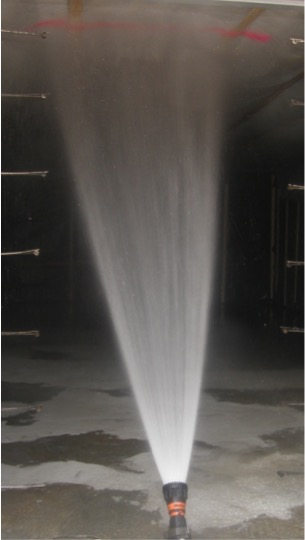
\includegraphics[width=0.75\columnwidth]{../Figures/Pictures/NF_example}
		\caption{Narrow fog stream from combination nozzle}
	\end{subfigure}
	\begin{subfigure}[b]{0.45\columnwidth}
		\centering
		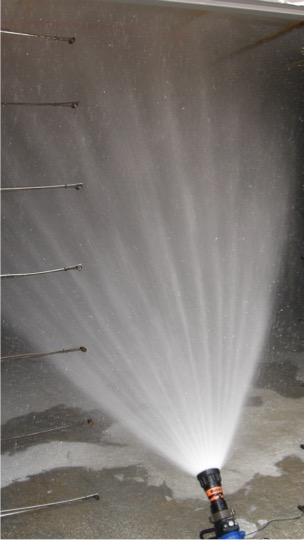
\includegraphics[width=0.75\columnwidth]{../Figures/Pictures/WF_example}
		\caption{Wide fog stream from combination nozzle}
	\end{subfigure}
	\\~\\
	\begin{subfigure}[b]{0.45\columnwidth}
		\centering
		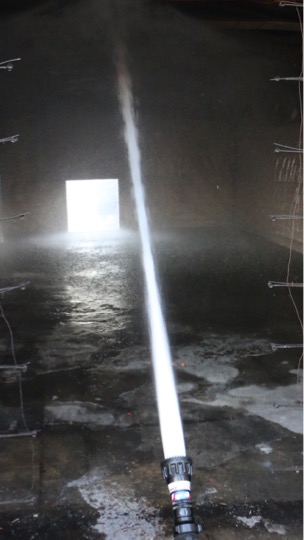
\includegraphics[width=0.75\columnwidth]{../Figures/Pictures/SS_70}
		\caption{Straight stream from combination nozzle}
	\end{subfigure}
	\begin{subfigure}[b]{0.45\columnwidth}
		\centering
		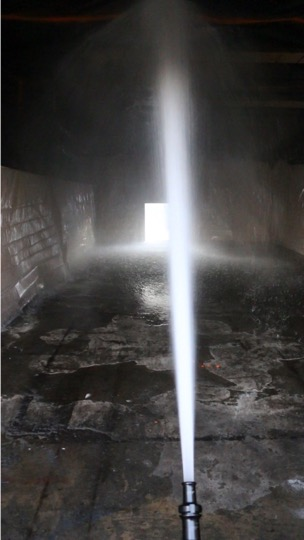
\includegraphics[width=0.75\columnwidth]{../Figures/Pictures/SB_70}
		\caption{Solid stream from 1~in smooth bore nozzle}
	\end{subfigure}
	\caption[Hose stream patterns used during experiments.]{The four types of hose stream patterns used during water flow experiments.}
	\label{fig:hose_streams}
\end{figure}

\clearpage

% =========================
% = EXPERIMENTAL OVERVIEW =
% =========================
\chapter{Experimental Overview}
\label{chap:exp_overview}
To study the impact of different hose stream and nozzle movement selections on air movement inside a structure, water flow experiments were conducted in two experimental structures designed to replicate typical residential structures. The experiments focused on studying the differences in the amount of air movement caused by specific combinations of four different hose stream patterns and four different nozzle movement patterns.

\section{Experimental Setup}
\label{sec:exp_setup}
The series of field experiments described in this report were conducted in two structures of similar design located at the Delaware County Emergency Services Training Center (ESTC) in Sharon Hill, PA. Differential pressure and temperature sensors were installed at ventilation points throughout the test structures to determine air velocity during the water flow experiments.  

\subsection{Test Structures}
\label{sec:test_structs}

\subsubsection{Construction}
\label{sec:construction}
Each test structure was built on a concrete slab as shown in Fig.~\ref{fig:struct_pics}. The Single Story Structure was designed to simulate a single-story residential structure, and the Two Story Structure was designed to simulate a two-story residential structure. The first floor of each structure had an outer wall composed of interlocking concrete blocks of equal side lengths of 0.61~m (2~ft). The joints and gaps between the blocks were filled with high temperature insulation.

\begin{figure}[!ht]
	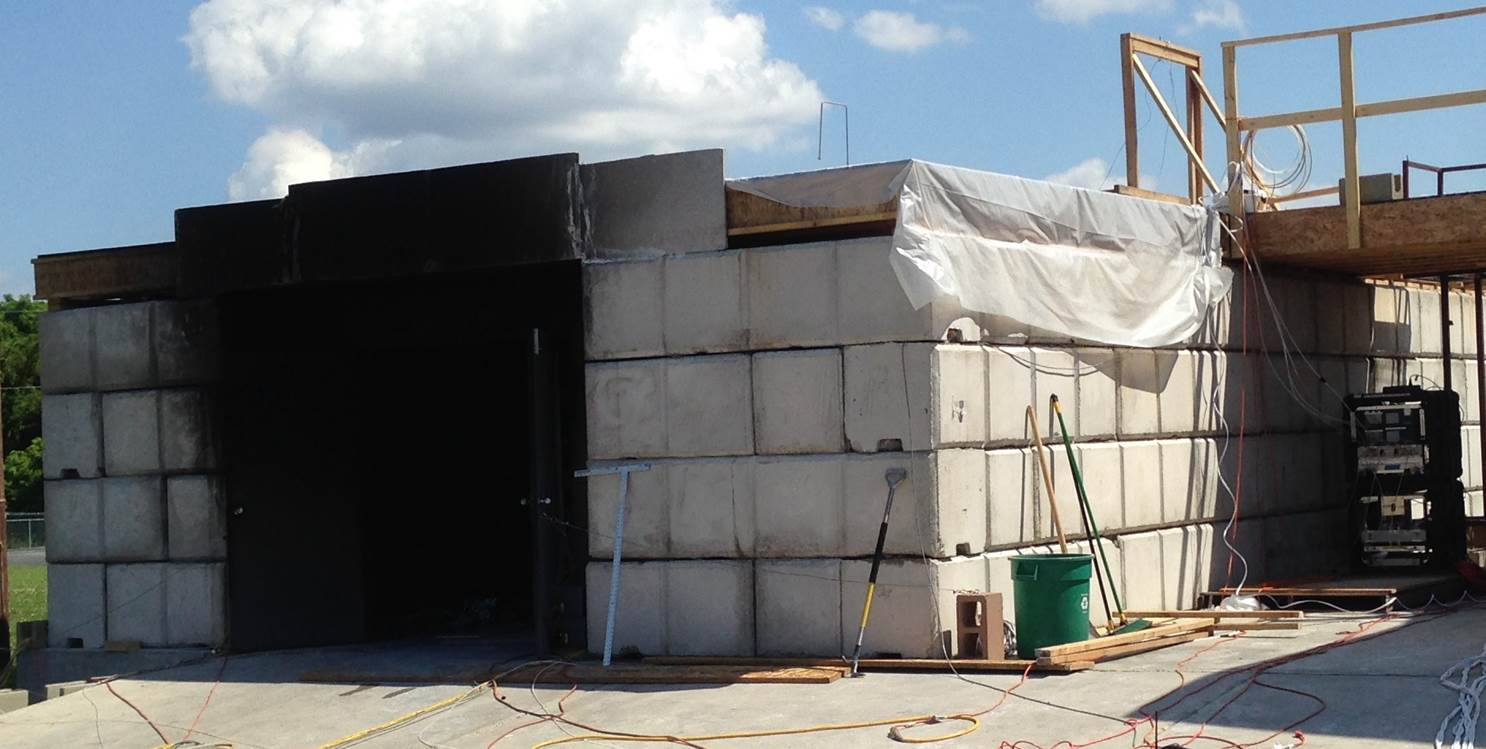
\includegraphics[width=5.25in]{../Figures/Pictures/east_structure}
	\\~\\
	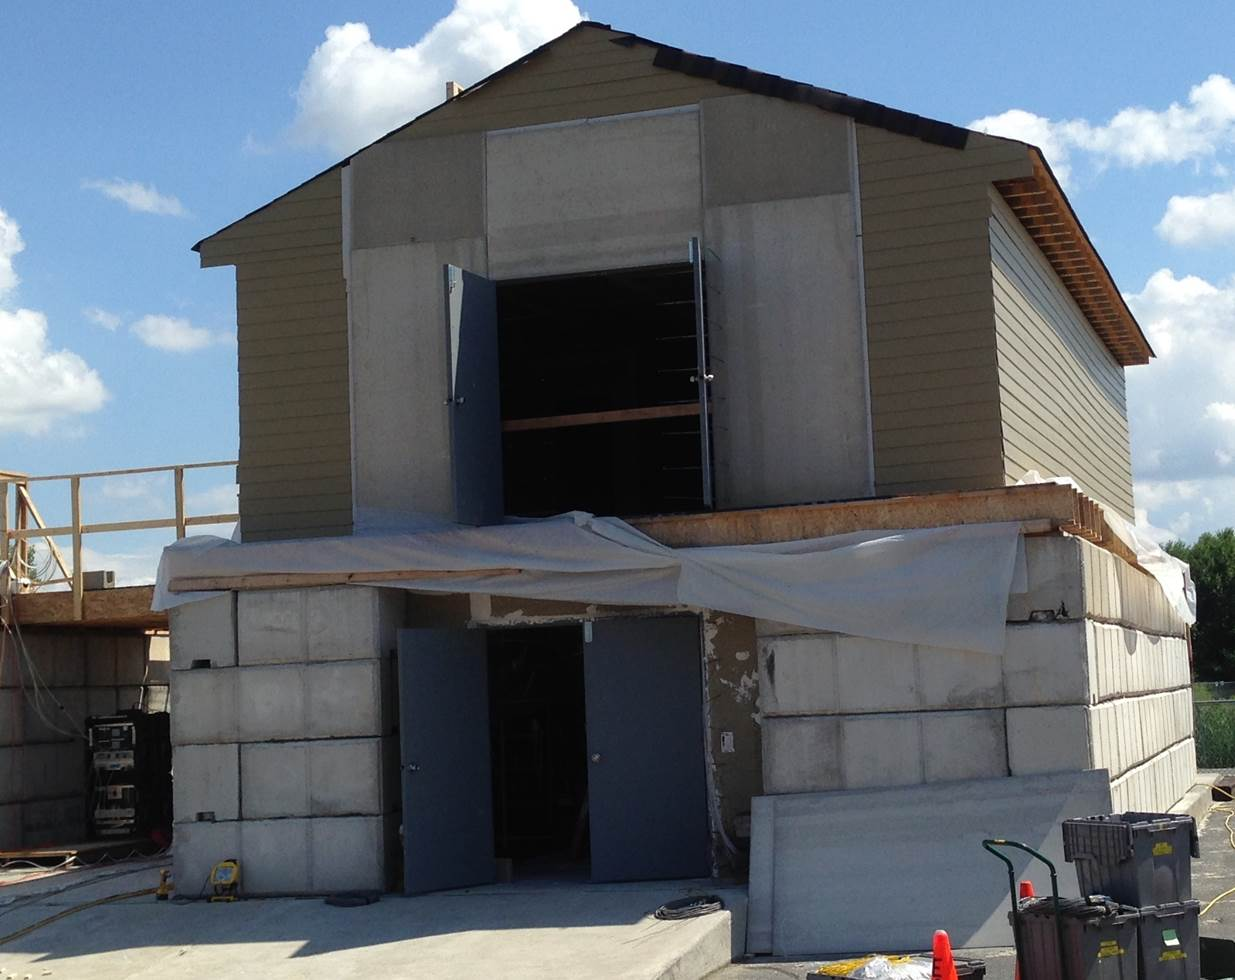
\includegraphics[width=5.25in]{../Figures/Pictures/west_structure}
	\caption[North side of the Single Story and Two Story Structures.]{North side of the Single Story (top) and Two Story (bottom) Structures.}
	\label{fig:struct_pics}
\end{figure}

The interior walls of the first floor of each structure were framed with steel studs set to 400~mm (16~in) centers and track and were lined with 13~mm (0.5~in) thick cement board. A layer of 16~mm (0.63~in) thick Type X gypsum board covered the cement board. Additionally, the ceiling was composed of two layers of 13~mm (0.5~in) thick cement board.
\FloatBarrier

The first floor ceiling support of each structure was composed of wood truss joist I-beams (TJIs) with a 298~mm (11.75~in) depth. Each TJI was composed of laminated veneer lumber flanges with a cross section of 29~mm (1.13~in) x 44~mm (1.75~in) and an 11~mm (0.43~in) thick oriented strand board web as shown in Fig.~\ref{fig:TJI}. Tongue and groove oriented strand board of 18.3~mm (0.72~in) thickness was screwed to the top of the TJIs.

\begin{figure}[!ht]
	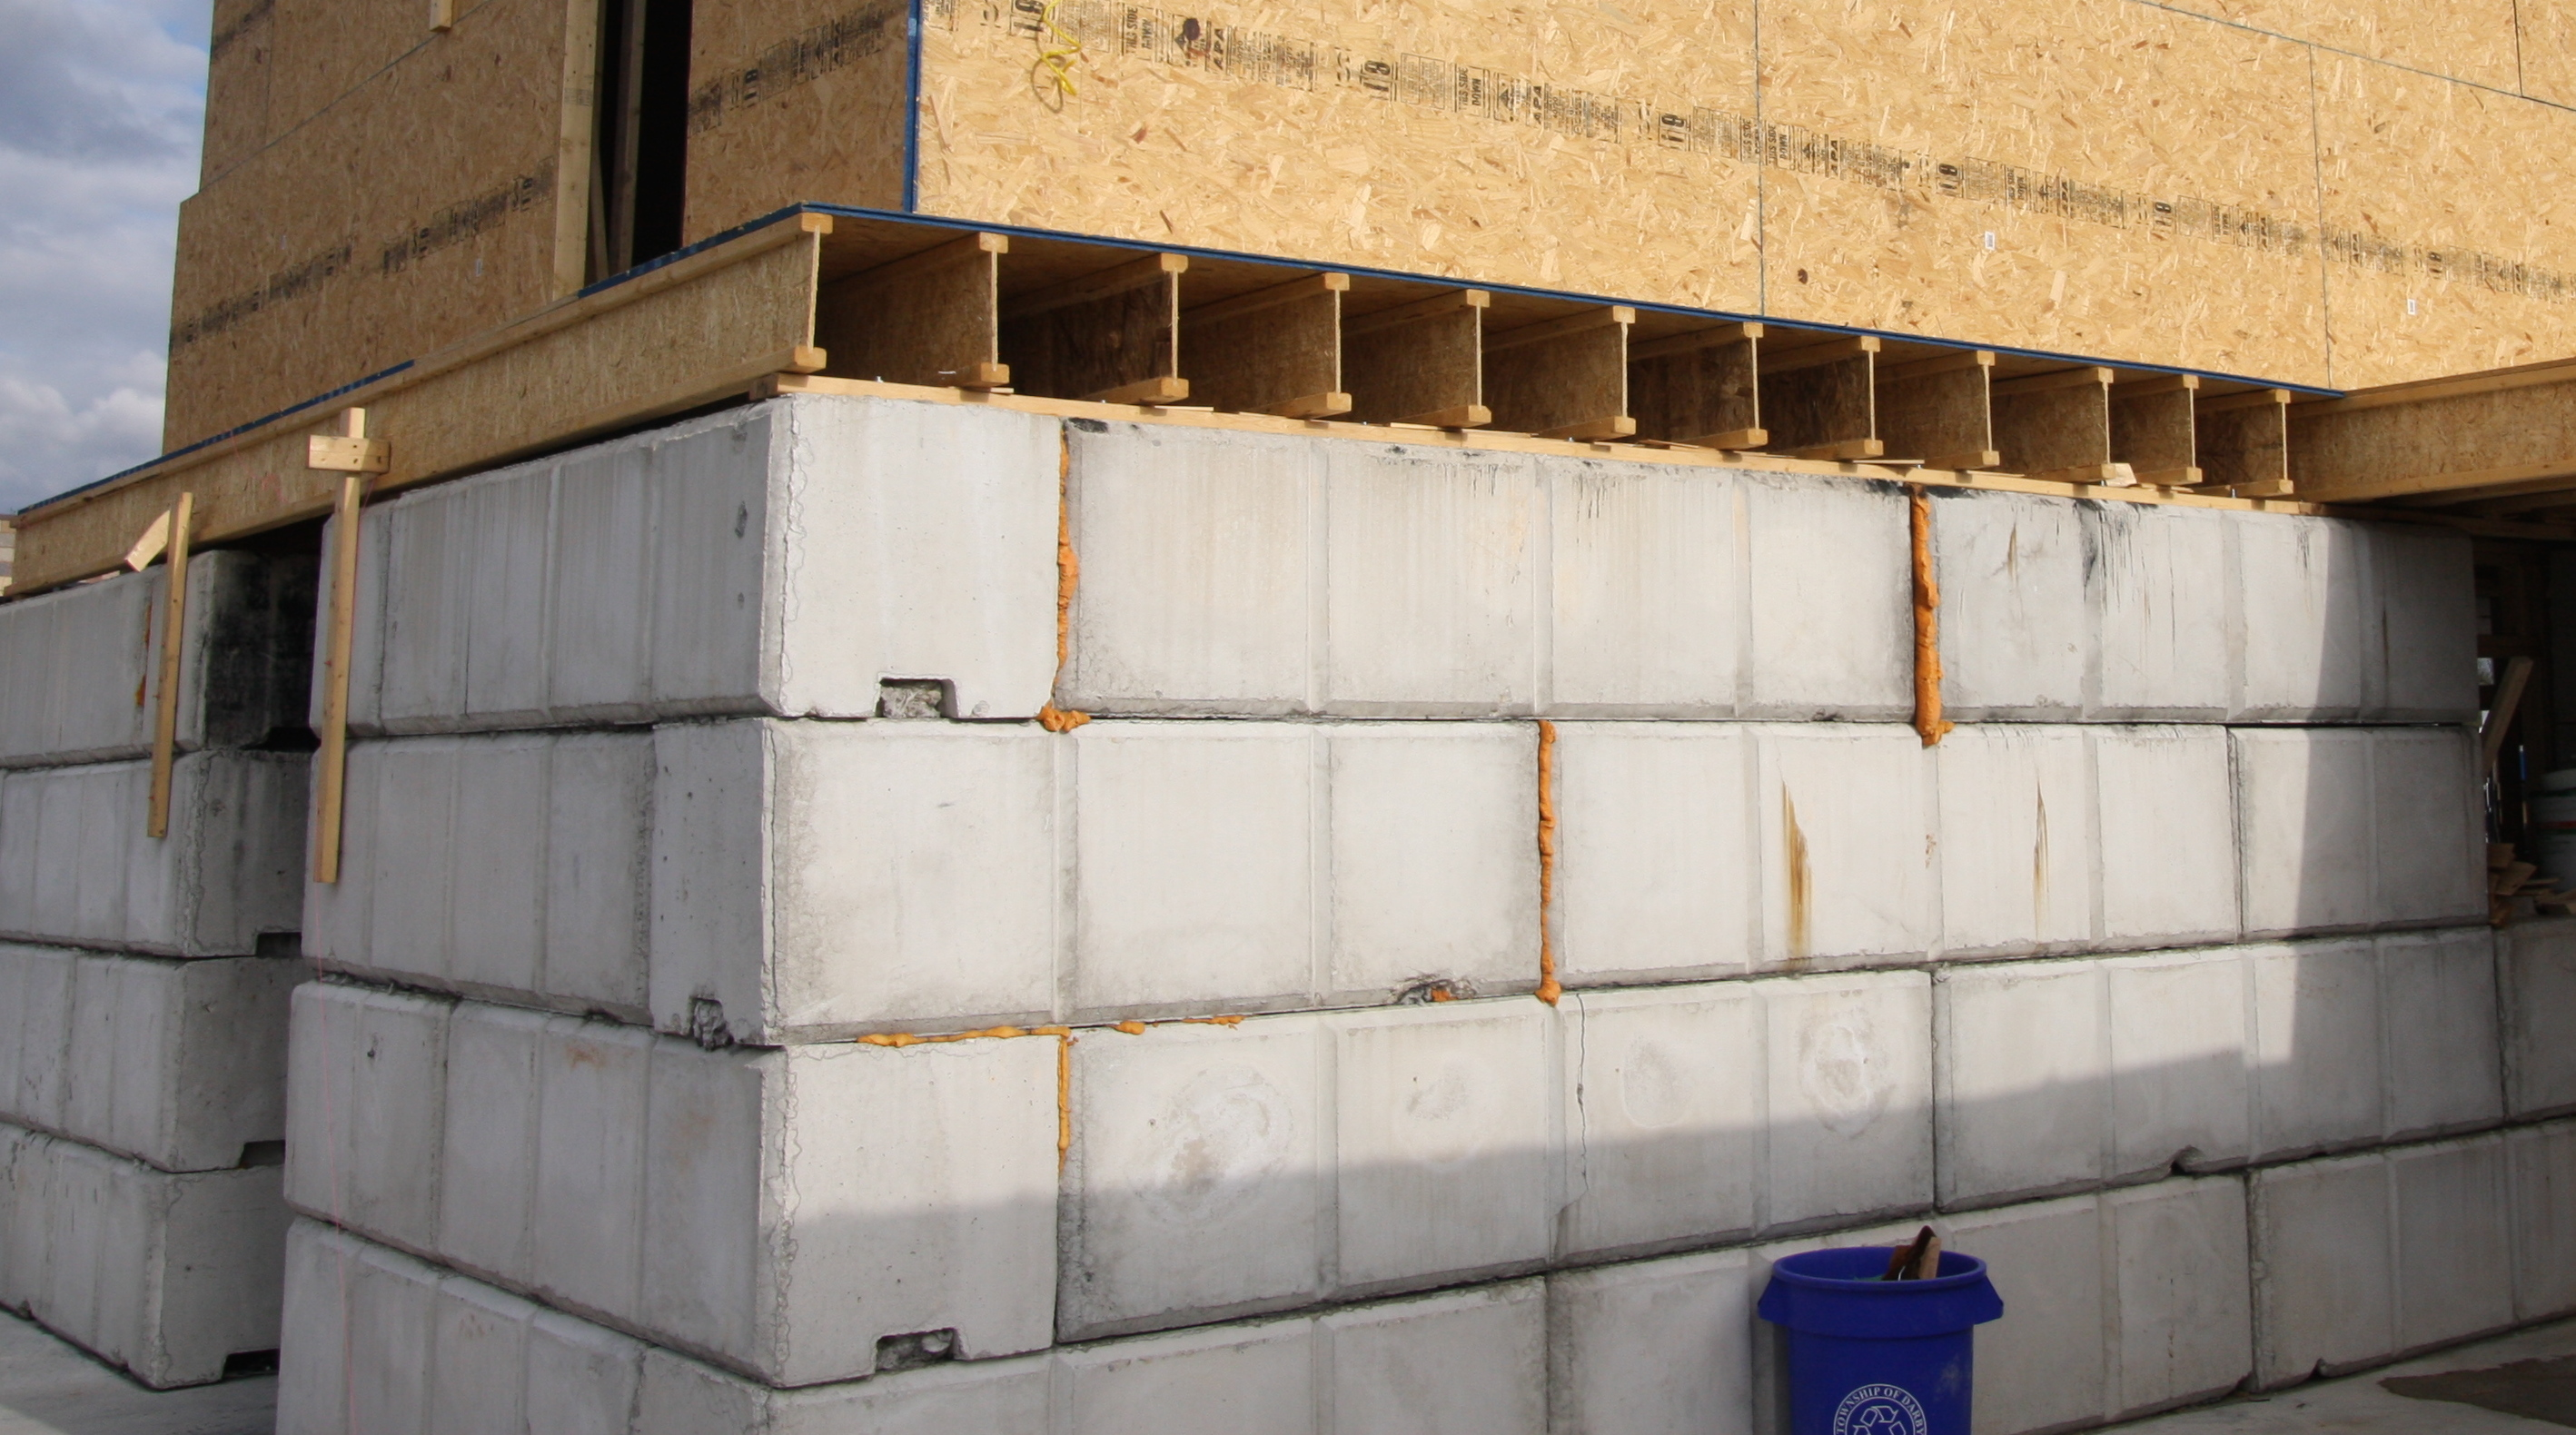
\includegraphics[width=\columnwidth]{../Figures/Pictures/TJI_support}
	\caption[TJI-constructed ceiling support of the Two Story Structure.]{First floor ceiling support of the Two Story Structure composed of wood truss joist I-beams. View is of the southeast corner of the structure.}
	\label{fig:TJI}
\end{figure}
\FloatBarrier

The second floor of the Two Story Structure was built on the wood ceiling support described above and was connected to the first floor by a stairwell. The walls of the second floor were wood-frame with nominal 51~mm (2~in) by 102~mm (4~in) studs set to 400~mm (16~in) centers. The interior walls were protected by 16~mm (0.63~in) fire rated gypsum board, 16~mm (0.63~in) durarock board, and a second layer of 16~mm (0.63~in) fire rated gypsum board. The exterior walls were protected with 11~mm (0.44~in) oriented strand board and 8~mm (0.31~in) fiber cement lap siding.

\subsubsection{Layout}
\label{sec:layout}
Dimensioned floor plans of the Single Story and Two Story Structures are presented in Fig.~\ref{fig:east_dimensioned_plan} and Fig.~\ref{fig:west_dimensioned_plan}, respectively.

The ceiling height of each structure was approximately 2.4~m (8~ft). The interior dimensions of the Single Story Structure were approximately 6.1~m (20~ft) by 11~m (36~ft), and the interior dimensions of the first and second floors of the Two Story Structure were 5.8~m (19~ft) by 10.7~m (35.1~ft) and 6.1~m (20~ft) by 10.9~m (35.8~ft), respectively. The stairs connecting the two floors of the Two Story Structure started 1.6~m (5.3~ft) off the south wall with a width of 1.2~m (4~ft) off the east wall and contained a 180~mm (7.25~in) rise and 190~mm (7.5~in) run.

The exterior doorways of each structure and the stairwell doorway on the second level of the Two Story Structure all contained doors that were opened or closed at certain instances during tests to change the ventilation pathways within the structure. All other doorways in the structures did not contain a door. In order to close these doorways, a sheet of gypsum board was used to cover the opening, and the doorway remained closed for the duration of the test procedure.
\clearpage

\begin{figure}[!ht]
	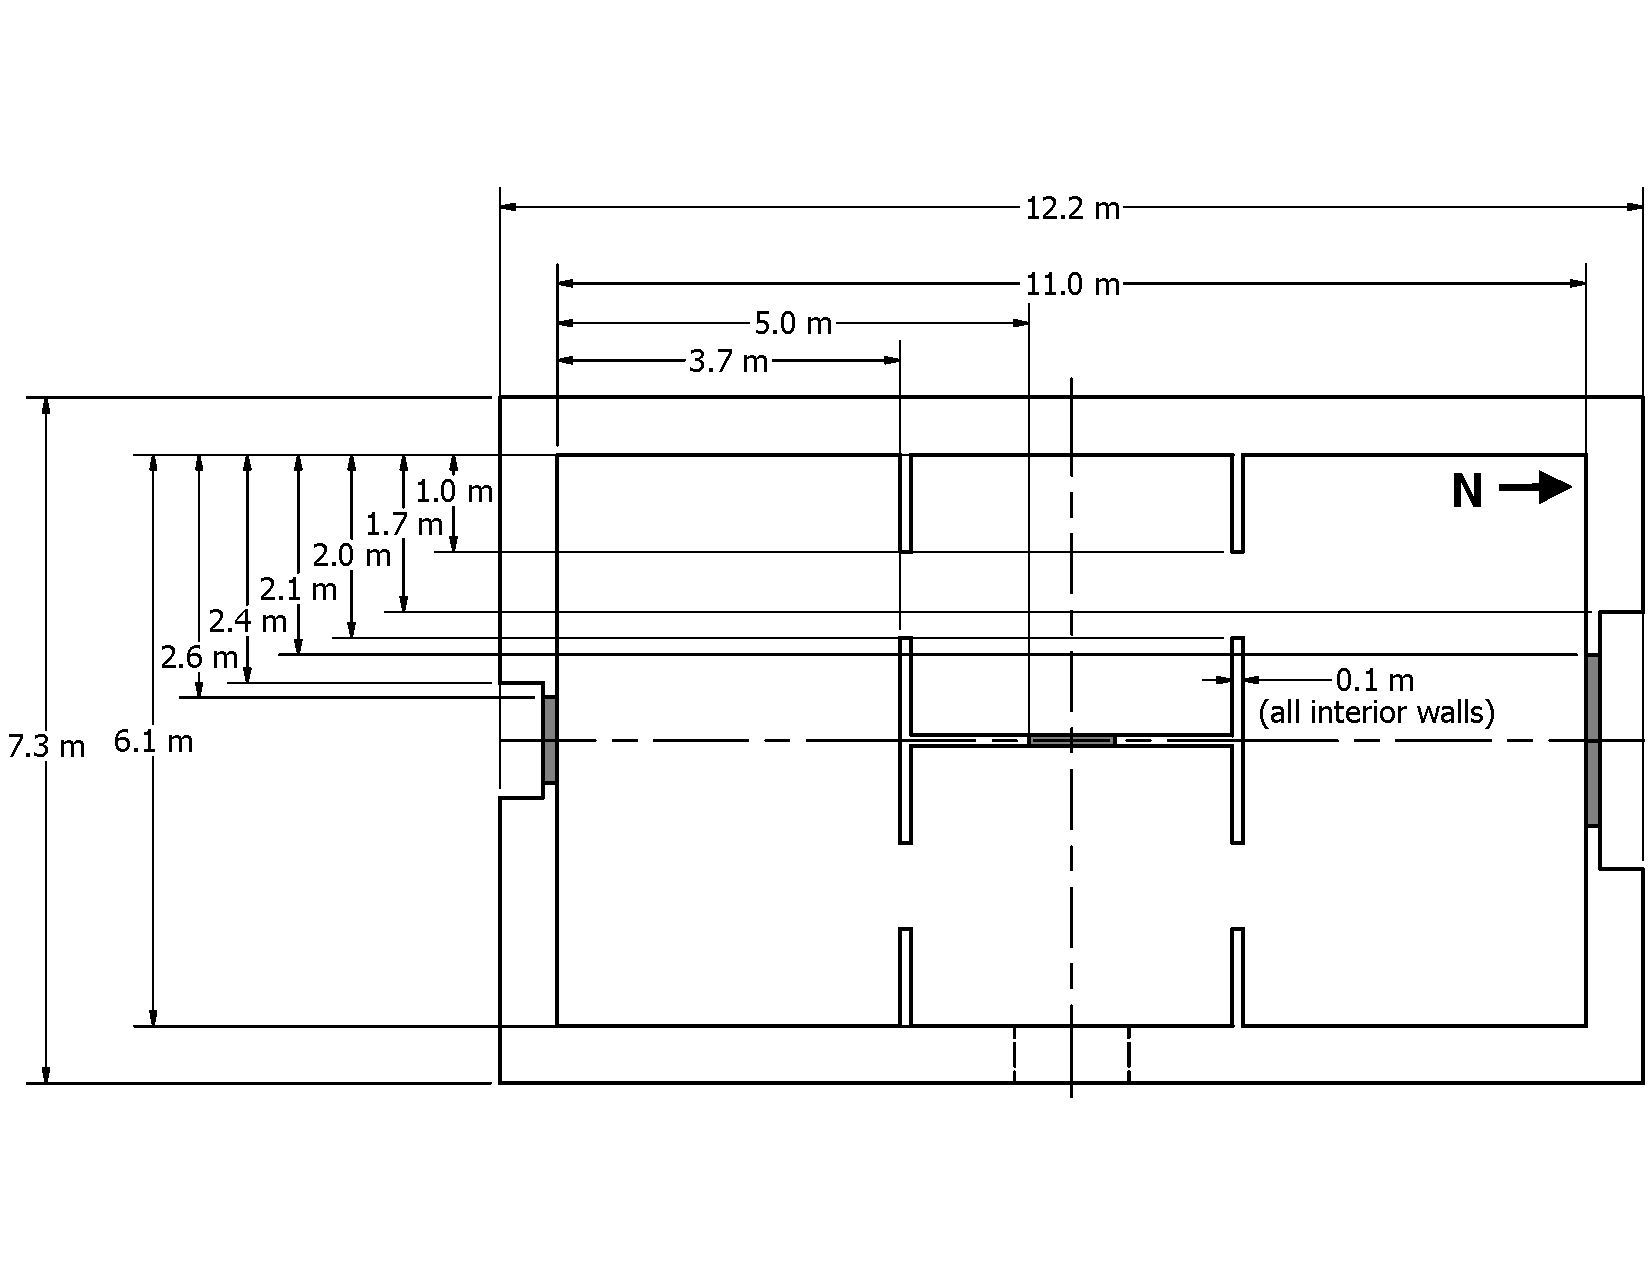
\includegraphics[width=\columnwidth]{../Figures/Floor_Plans/East_Test_Structure_Dimensioned_Full}
	\caption[Dimensioned floor plan of the Single Story Structure.]{Dimensioned floor plan of the Single Story Structure. Interior dimensions are symmetric across horizontal and vertical centerlines.}
	\label{fig:east_dimensioned_plan}
\end{figure}

\begin{figure}[!ht]
	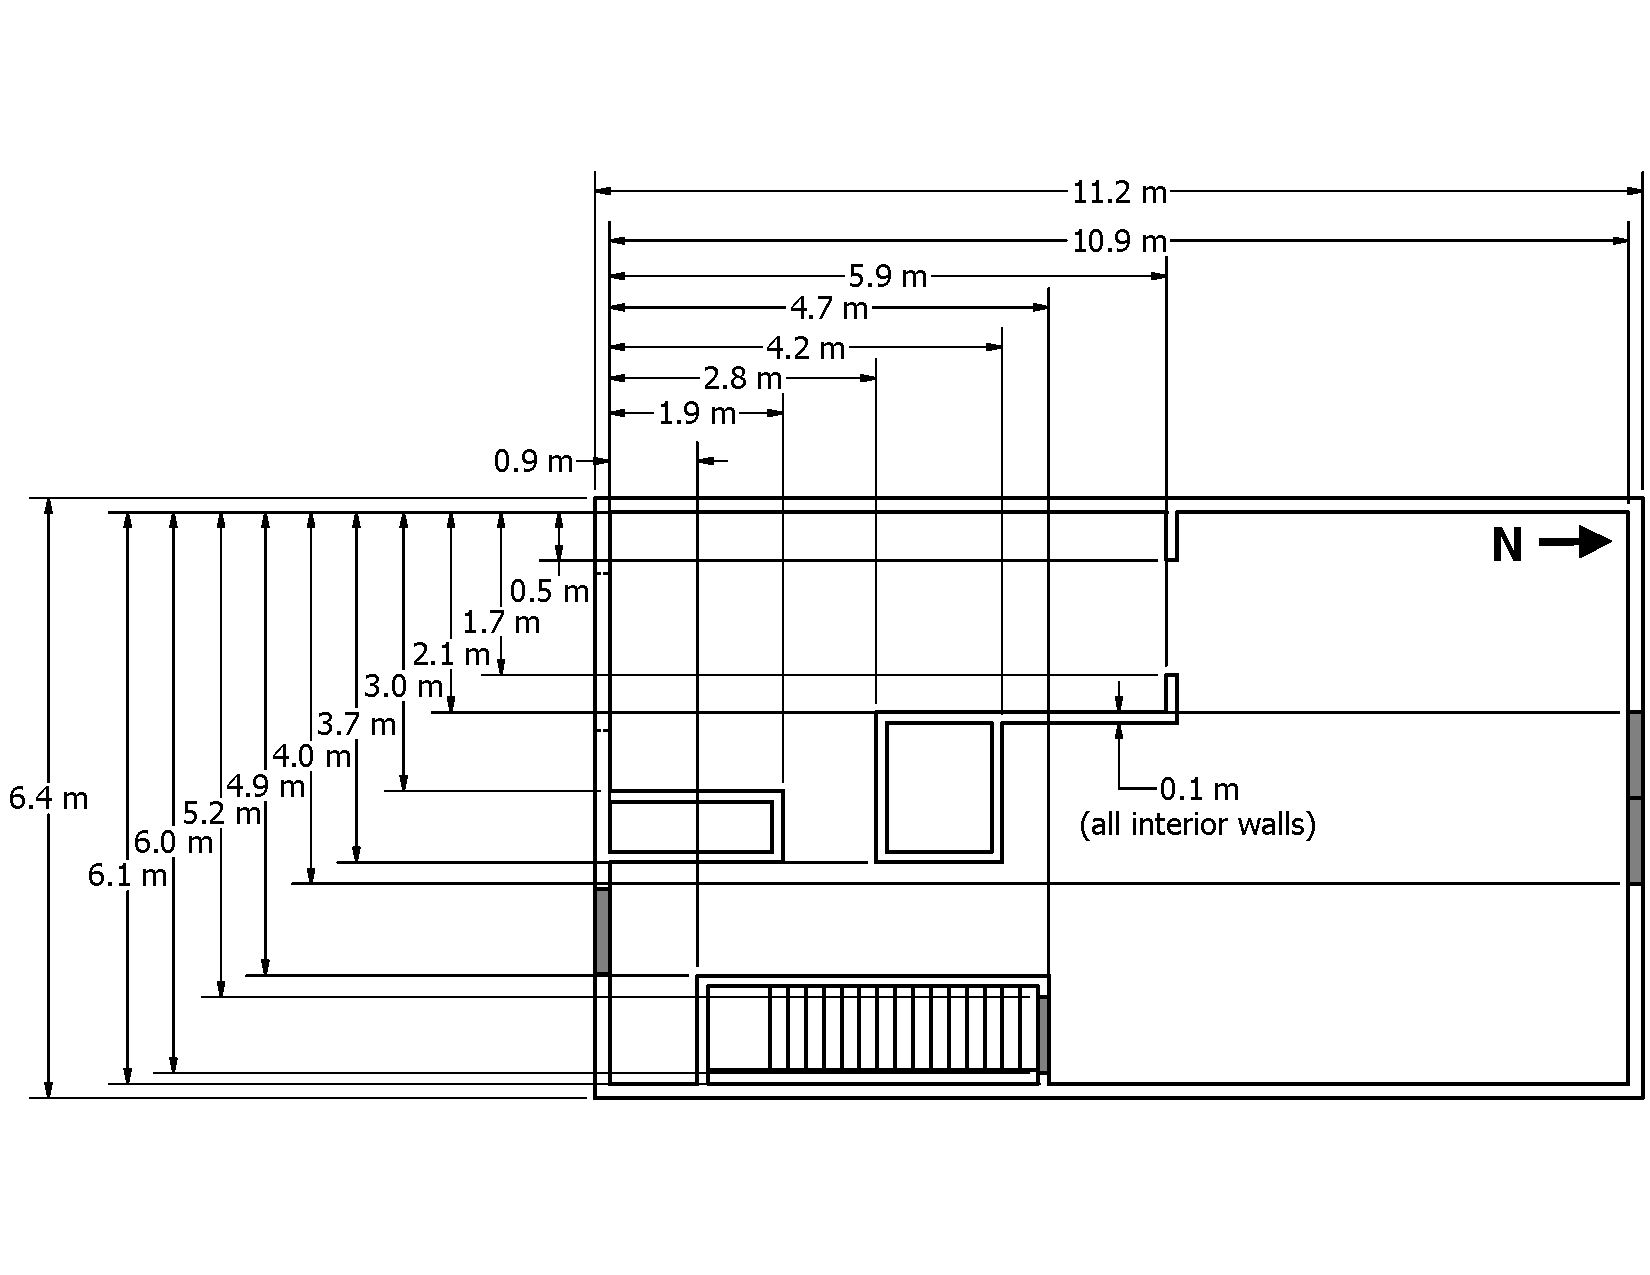
\includegraphics[width=\columnwidth]{../Figures/Floor_Plans/West_Structure_2nd_Floor_Dimensioned_Full}
	\\~\\
	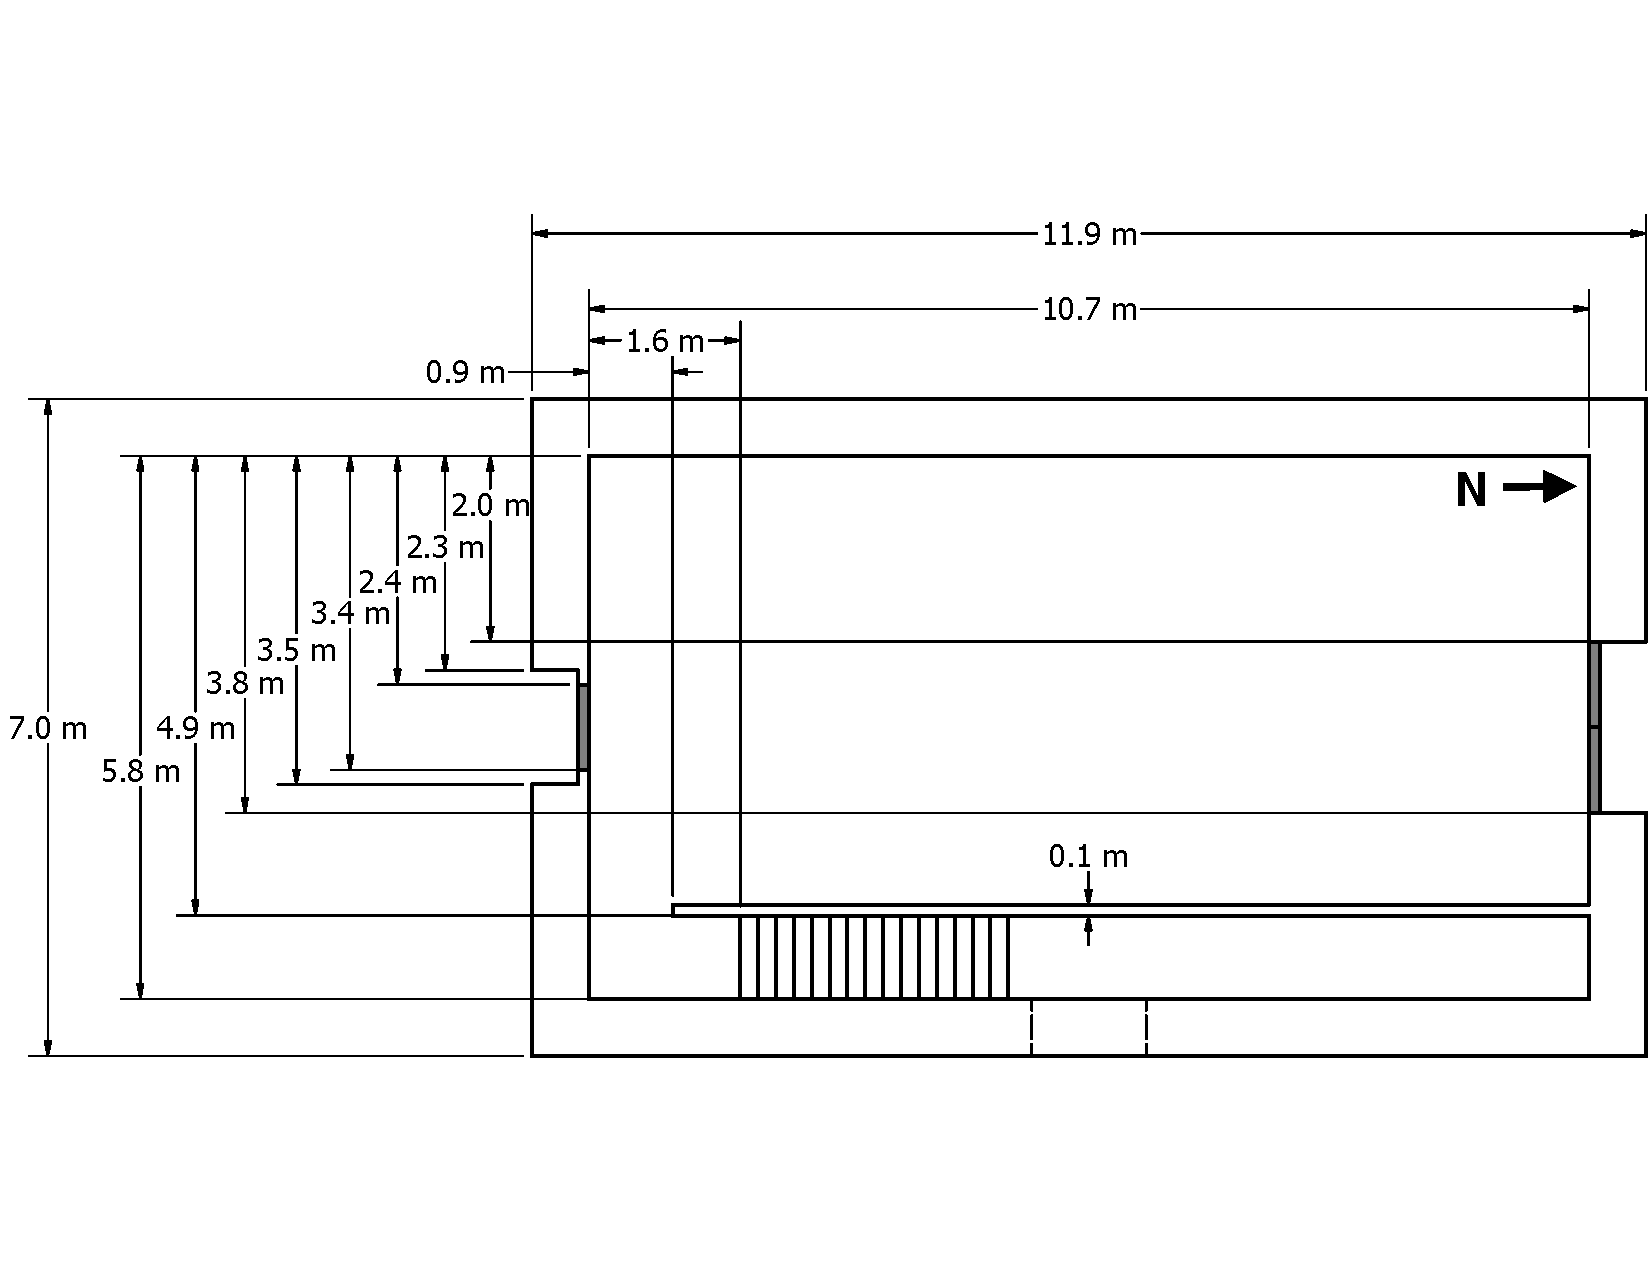
\includegraphics[width=\columnwidth]{../Figures/Floor_Plans/West_Structure_1st_Floor_Dimensioned_Full}
	\caption[Dimensioned floor plan of the first and second floors of the Two Story Structure.]{Dimensioned floor plan of the second floor (top) and first floor (bottom) of the Two Story Structure.}
	\label{fig:west_dimensioned_plan}
\end{figure}

\clearpage

\subsection{Instrumentation}
\label{sec:instrumentation}
For every experiment, gas velocity at an interior doorway was calculated using differential pressure transducers connected to bi-directional velocity probes~\cite{McCaffrey:Combustion_and_Flame}. An array of six bi-directional probes located at the northeast interior doorway of the Single Story Structure is pictured below in Fig.~\ref{fig:BDPs}. A single thermocouple was attached to each bi-directional probes to measure the gas temperature to be used in conjunction with the pressure measurement to calculate velocity. Every thermocouple attached to the bi-directional probes was an exposed-bead, Chromel-Alumel (type K) with a 1.0~mm (0.04 in) diameter. The thermocouple wire was sheathed in a 3.2~mm (0.13 in) diameter Inconel shield that started at the exposed bead and was 0.76~m (2.5~ft) in length. 

The approximate locations of the bi-directional probes are annotated in the plan views of the experimental setups for the Single Story and Two Story Structures (Figs.~\ref{fig:east_setup}--\ref{fig:flow_path_2}) in Section~\ref{sec:exp_procedure}. To minimize potential measurement errors due to external environmental conditions (i.e., wind), only velocity data measured by bi-directional probes located at interior doorways are considered in this report. The set of bi-directional probes at the northeast interior doorway of the Single Story Structure, denoted as ``A6'' and pictured in Fig.~\ref{fig:BDPs}, contained six probes located at distances of 0.30~m (1.0~ft), 0.60~m (2.0~ft), 0.90~m (3.0~ft), 1.20~m (3.9~ft), 1.50~m (4.9~ft), and 1.80~m (5.9~ft) below the soffit of the doorway. The set of bi-directional probes at the interior doorway in the Two Story Structure, denoted as ``A10'', contained eight probes located at distances of 0.08~m (0.25~ft), 0.34~m (1.1~ft), 0.61~m (2.0~ft), 0.88~m (2.9~ft), 1.15~m (3.7~ft), 1.42~m (4.7~ft), 1.68~m (5.5~ft), and 1.95~m (6.4~ft) below the soffit of the corresponding doorway.

A discussion of uncertainties for each type of measurement in this report can be found in Section~\ref{sec:uncertainty}.

\begin{figure}[!ht]
	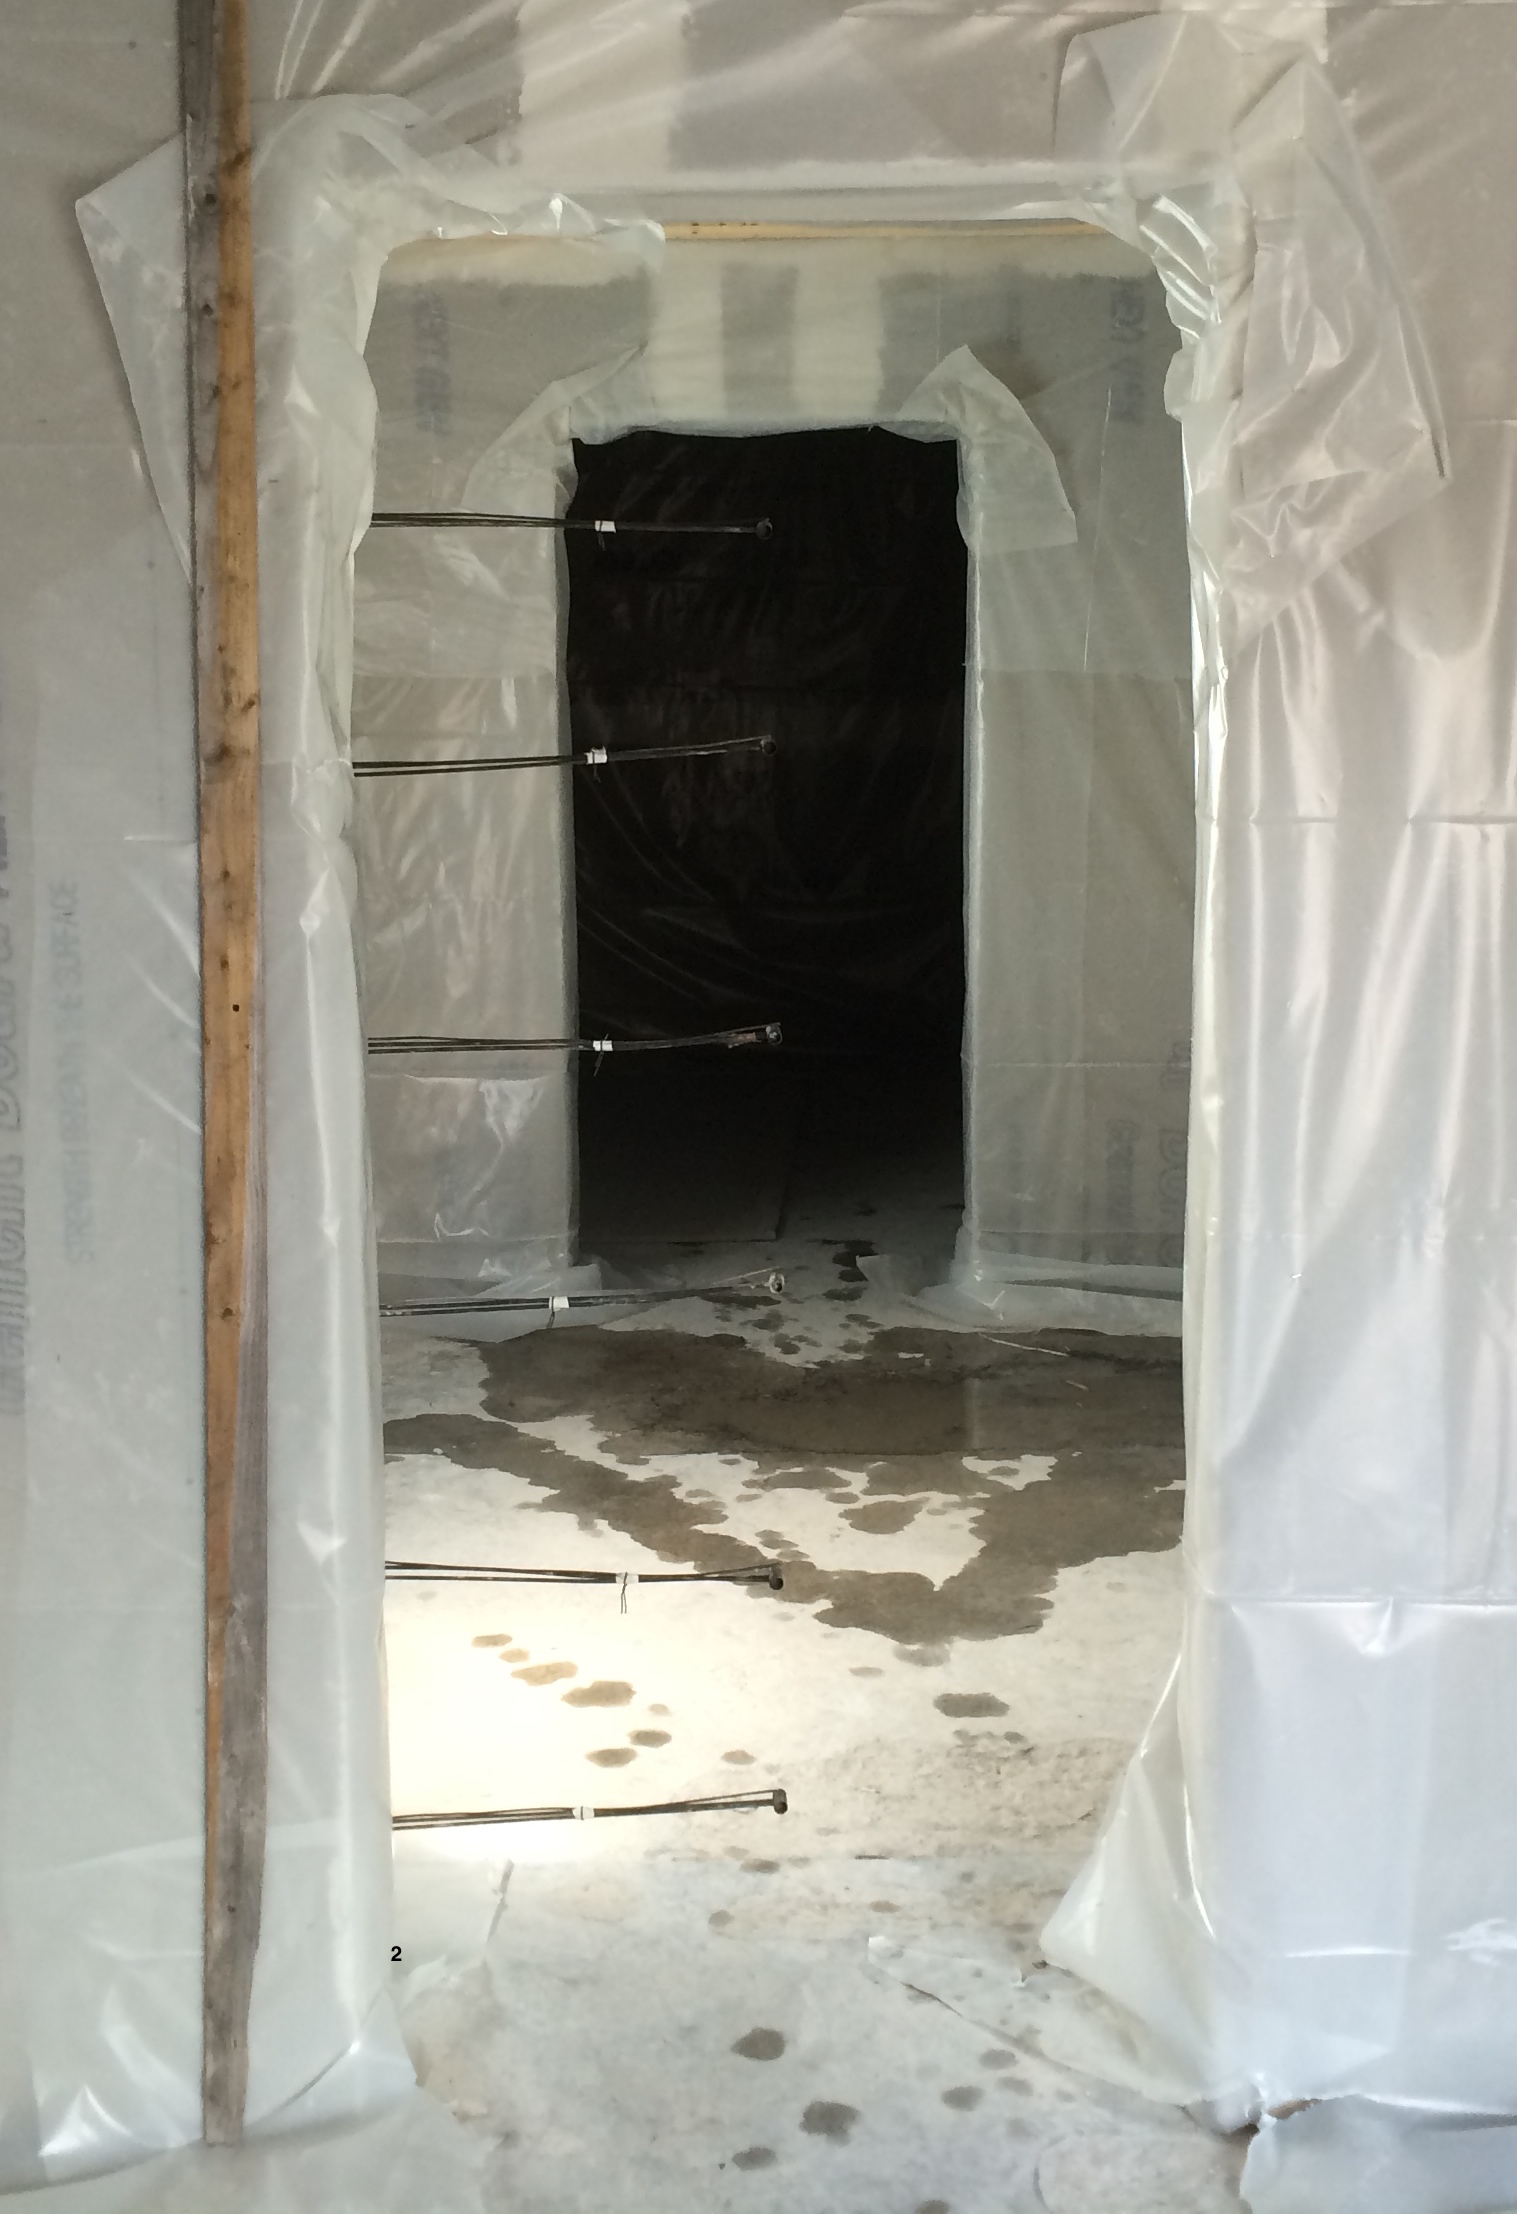
\includegraphics[width=3.5in]{../Figures/Pictures/BDPs_east}
	\caption[Array of bi-directional probes at interior doorway in Single Story Structure.]{Array of bi-directional probes located at the northeast interior doorway in the Single Story Structure. View is looking at the north side of the doorway.}
	\label{fig:BDPs}
\end{figure}
\FloatBarrier

\subsection{Uncertainty}
\label{sec:uncertainty}
There are different components of uncertainty in the length, differential pressure, flow rate, and gas velocity reported here. Uncertainties are grouped into two categories according to the method used to estimate them. Type A uncertainties are those which are evaluated by statistical methods, and Type B are those which are evaluated by other means~\cite{Taylor&Kuyatt:1994}. Type B analysis of systematic uncertainties involves estimating the upper (+a) and lower (-a) limits for the quantity in question such that the probability that the value would be in the interval ($\pm$a) is essentially 100~\%. After estimating uncertainties by either Type A or B analysis, the uncertainties are combined in quadrature to yield the combined standard uncertainty. Then, the combined standard uncertainty is multiplied by a coverage factor of two, which results in the expanded uncertainty with a 95~\% confidence interval (2$\sigma$). For some of these components, such as the zero and calibration elements, uncertainties are derived from referenced instrument specifications. For other components, referenced research results and past experience with the instruments provided input in the uncertainty determination. 

\subsubsection{Length Measurements}
Each length measurement was taken carefully. Length measurements such as the room dimensions, instrumentation array locations, and fire apparatus (e.g., nozzle, sprinkler, or fan) placement were made with a hand held laser measurement device which has an accuracy of $\pm$6.0~mm (0.25~in) over a range of 0.61~m (2.0~ft) to 15.3~m (50.0~ft)~\cite{StanleyTools}.  However, conditions affecting the measurement, such as levelness of the device, yields an estimated uncertainty of $\pm$0.5~\% for measurements in the 2.0~m (6.6~ft) to 10.0~m (32.8~ft) range. Steel measuring tapes with a resolution of $\pm$0.5~mm (0.02~in) were used to locate individual sensors within a measurement array. The steel measuring tapes were manufactured in compliance with NIST Manual 44, which specifies a tolerance of $\pm$1.6~mm (0.06~in) for 9.1~m (30~ft) tapes and $\pm$6.4~mm (0.25~in) for 30.5~m (100~ft) tapes~\cite{Butcher:2012}.

\subsubsection{Bi-Directional Probes}
Bi-directional probes with pressure transducers and single thermocouples were used to measure the gas velocity. Inconel-sheathed, exposed bead, type K thermocouples were co-located with each probe. A gas velocity measurement study examining the doorway flow of pre-flashover compartment fires yielded expanded uncertainty measurements ranging from $\pm0.14$ to $\pm0.22$ for bi-directional probes of similar design~\cite{Bryant:FSJ2009}. The total expanded uncertainty for gas velocity in these experiments is estimated to be $\pm18$~\%.   

\subsubsection{Water Flow Rate}
Water flow rate was measured with a pressure and flow meter combination shown in Fig.~\ref{fig:flow_meter}. The meter consisted of a section of 63.5~mm (2.5~in) cast aluminum pipe with a 0 to 4.1~MPa (600~psi) pressure transducer and a paddlewheel type flow sensor with a range of 0 to 4800~lpm (1250~gpm). The pressure transducer and paddlewheel were both connected to the battery operated control box where the pressure transducer voltage was converted to a pressure and the paddlewheel pulse count was converted to a volumetric flow rate. The manufacturer reports a $\pm5$~\% calibration expanded uncertainty for the flow sensor and $\pm3$~\% for the pressure sensor~\cite{Akron:2009}. The pressure transducer was calibrated with a known analog pressure gauge. The flow meter was calibrated by capturing water over time and measuring that mass of water to determine the flow rate. The total expanded uncertainty was estimated at $\pm10$~\%. 

\begin{figure}[!ht]
	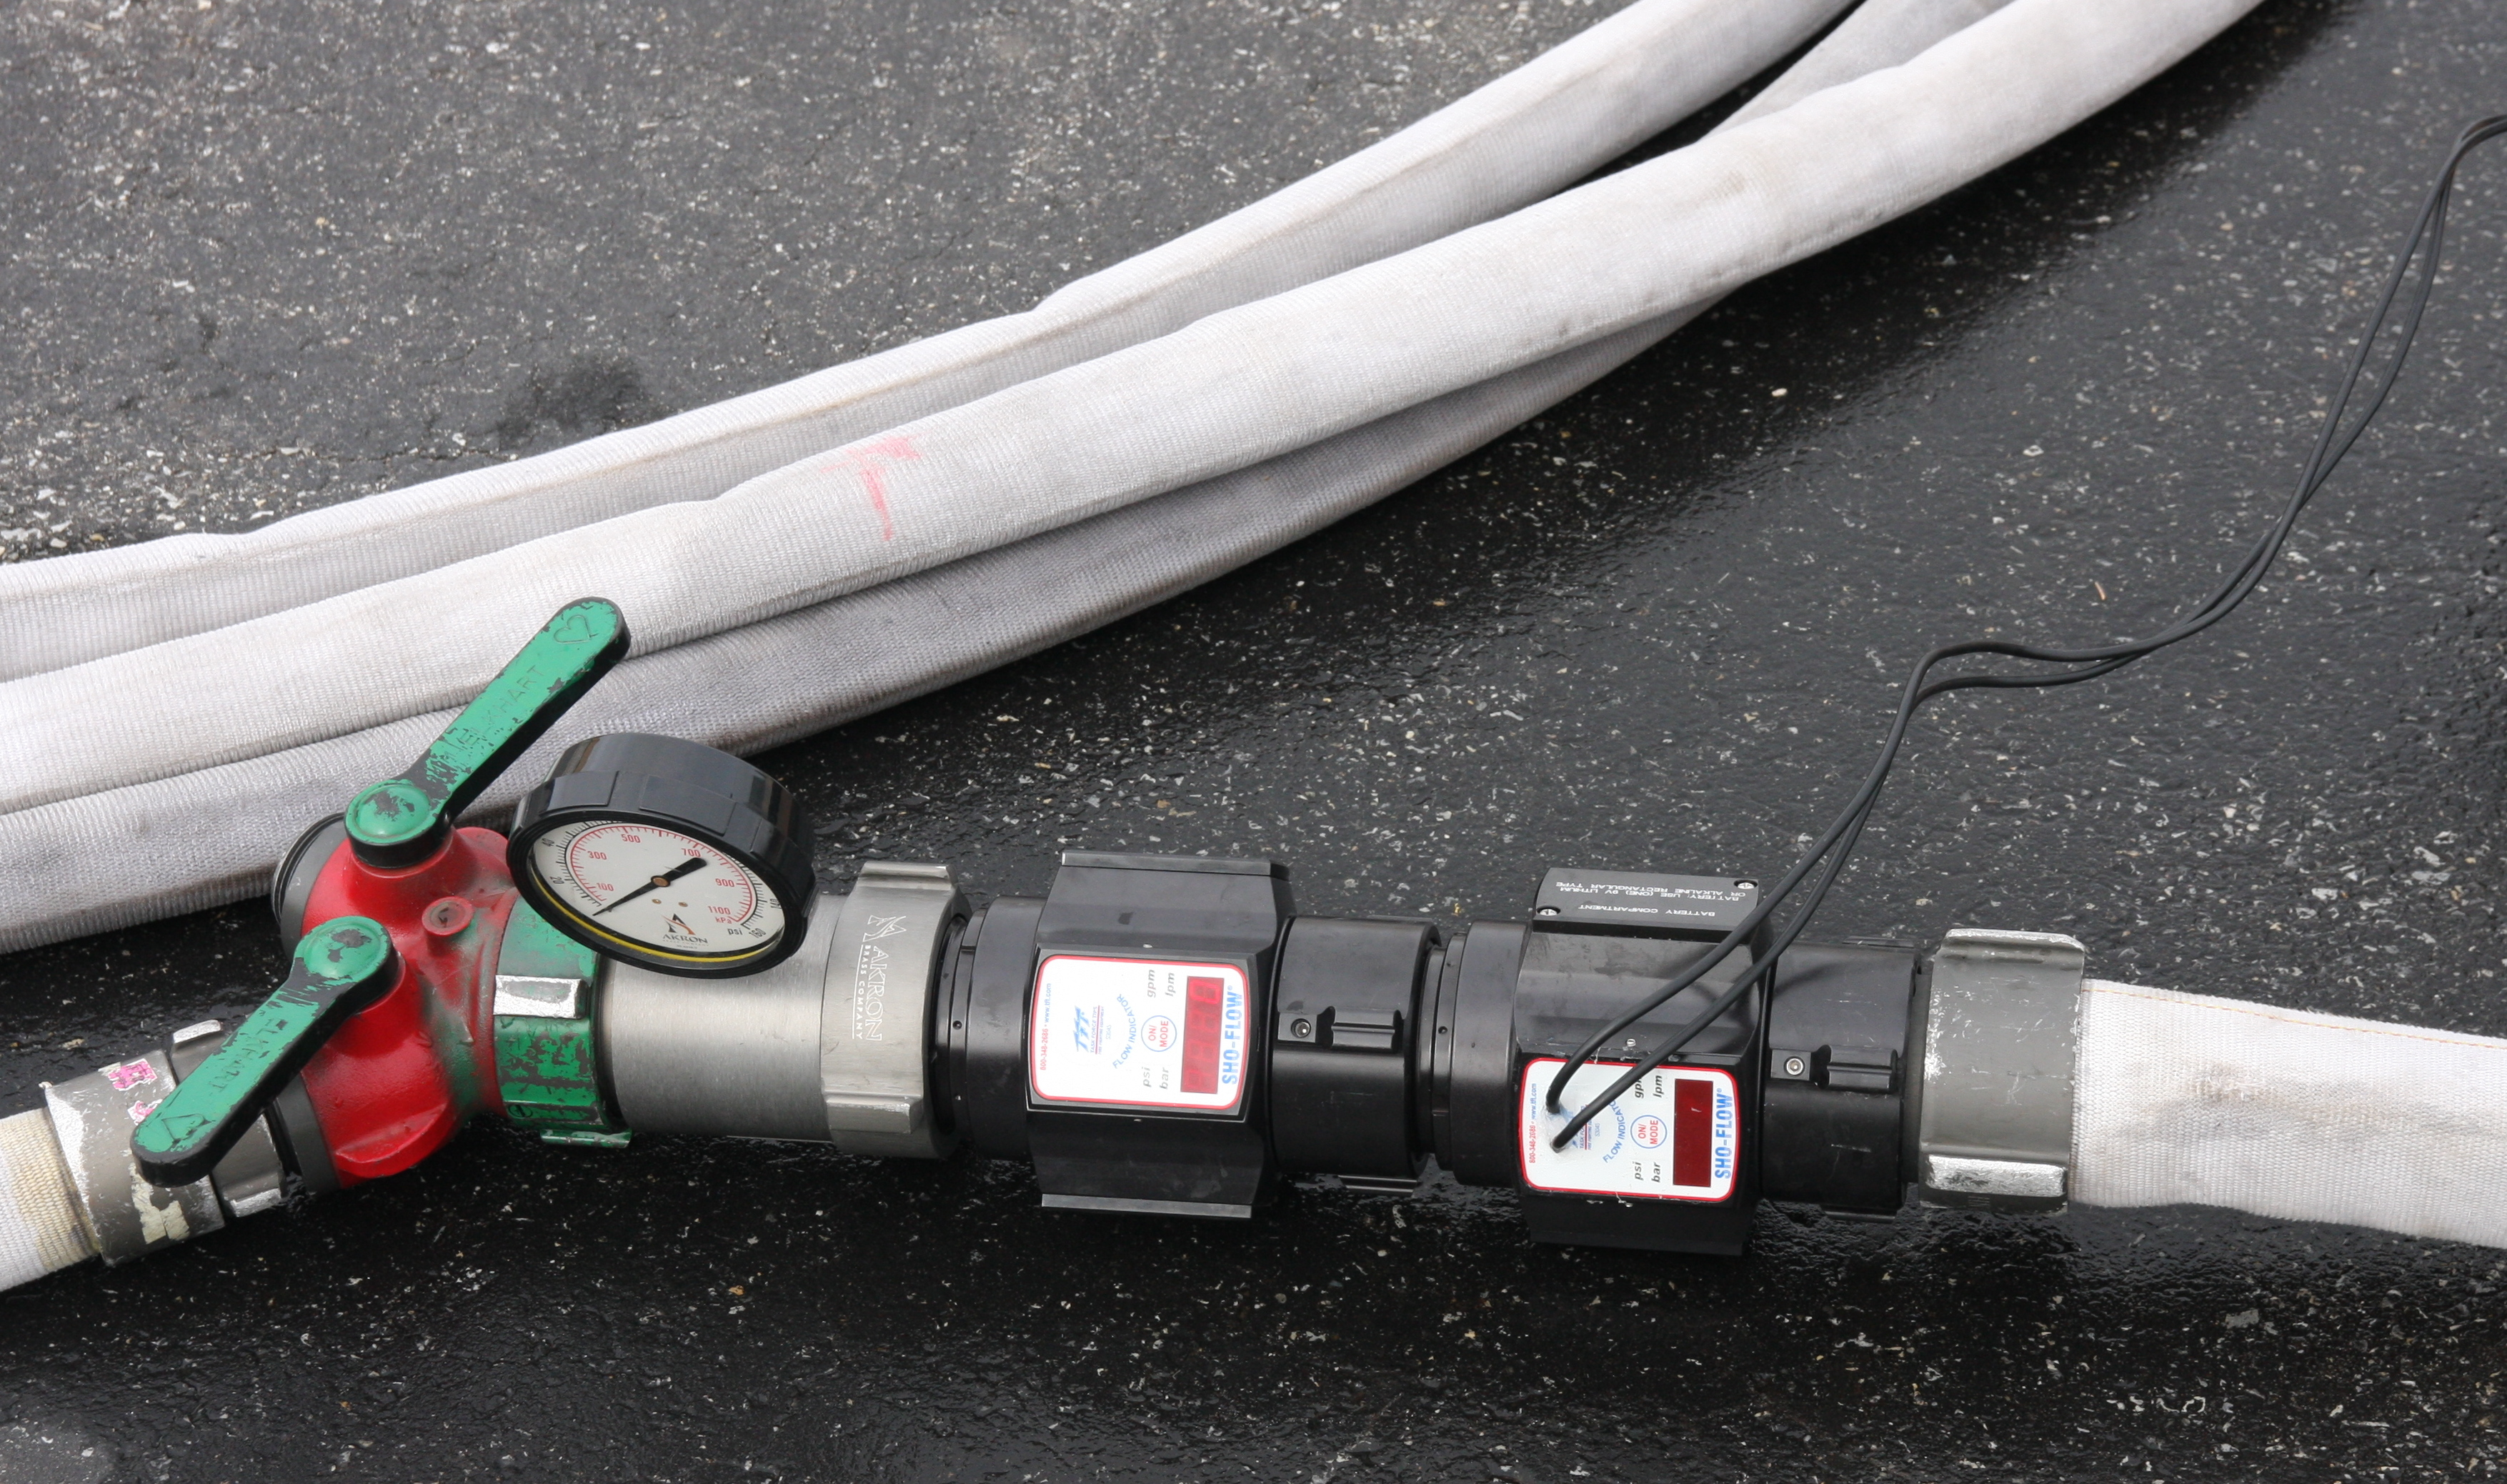
\includegraphics[width=3in]{../Figures/Pictures/flow_meter}
	\caption[Flow meter used to measure flow rate during experiments.]{Pressure and flow meter combination used to measure water flow rate during the experiments.}
	\label{fig:flow_meter}
\end{figure}
\FloatBarrier

\section{Experimental Procedure}
\label{sec:exp_procedure}
Every experiment discussed in this report involved discharging water at a set flow rate from a combination nozzle in a straight, narrow fog, or wide fog stream pattern or from a smooth bore nozzle with a 1~in tip in a solid stream pattern. Specific doors were opened or closed before and/or during the tests to change the ventilation within the structure. 

A total of seven experimental series, summarized in Table~\ref{table:test_matrix}, were conducted to study the impact of different hose stream and nozzle motion patterns on gas movement in a structure; three used a combination nozzle attached to a monitor to flow water at approximately 120~gpm, three used a combination nozzle attached directly to a 1.75~in handline to flow water at approximately 120~gpm (Fig.~\ref{fig:monitor+handline}), and one used both a combination nozzle and a smooth bore nozzle attached to a monitor to flow water at approximately 180~gpm. Experiments that used a monitor to flow water always applied the stream in a fixed position and were focused on changing the location of water application in addition to the stream pattern. The experiments that used a combination nozzle attached directly to a 1.75~in handline to flow water focused on impact of the motion of the nozzle.

\begin{table}[!ht]
\caption{Summary of the seven experimental test series}
\begin{tabular}{ccclll}
 \toprule
\textbf{Test \#} & \textbf{Appliance} & \textbf{Structure} & 
\begin{tabular}{@{}l} \textbf{Flow Path} \\ \textbf{Configuration} \end{tabular} &
\textbf{Streams} & \textbf{Nozzle Motion} \\
\midrule
1 & Monitor & \begin{tabular}{@{}c@{}} Single \\ Story \end{tabular} & U-shaped & 
\begin{tabular}{@{}l} Straight, \\ Narrow fog, \\ Wide fog \\ (120~gpm) \end{tabular} & 
Fixed position 
\\~\\
2 & Monitor & \begin{tabular}{@{}c@{}} Two \\ Story \end{tabular} & 
\begin{tabular}{@{}l} Nozzle lower \\ level north side, \\ Exhaust lower \\ level south side \\ and upper level \\ north side \end{tabular} & 
\begin{tabular}{@{}l} Straight, \\ Narrow fog, \\ Wide fog \\ (120~gpm) \end{tabular} & Fixed position
\\~\\
3 & Monitor & \begin{tabular}{@{}c@{}} Two \\ Story \end{tabular} & 
\begin{tabular}{@{}l} Nozzle lower \\ level north side, \\ Exhaust upper \\ level north side \end{tabular} & 
\begin{tabular}{@{}l} Straight, \\ Narrow fog, \\ Wide fog \\ (120~gpm) \end{tabular} & Fixed position
\\~\\
4 & Monitor & \begin{tabular}{@{}c@{}} Two \\ Story \end{tabular} & 
\begin{tabular}{@{}l} Nozzle lower \\ level north side, \\ Exhaust upper \\ level north side \end{tabular} & 
\begin{tabular}{@{}l} Straight, \\ Solid \\ (180~gpm) \end{tabular} & Fixed position
\\~\\
5 & Handline & \begin{tabular}{@{}c@{}} Single \\ Story \end{tabular} & U-shaped & 
\begin{tabular}{@{}l} Straight, \\ Narrow fog, \\ Wide fog \\ (120~gpm) \end{tabular} & 
\begin{tabular}{@{}l} Fixed at ceiling, \\ Rotated CW, \\ Rotated CCW \end{tabular}
\\~\\
6 & Handline & \begin{tabular}{@{}c@{}} Two \\ Story \end{tabular} & 
\begin{tabular}{@{}l} Nozzle lower \\ level north side, \\ exhaust lower \\ level south side \\ and upper level \\ north side \end{tabular} & 
\begin{tabular}{@{}l} Straight, \\ Narrow fog, \\ Wide fog \\ (120~gpm) \end{tabular} & 
\begin{tabular}{@{}l} Fixed at ceiling, \\ Sweeping ceiling, \\ Rotated CW, \\ Rotated CCW \end{tabular}
\\~\\
7 & Handline & \begin{tabular}{@{}c@{}} Two \\ Story \end{tabular} & 
\begin{tabular}{@{}l} Nozzle lower \\ level north side, \\ Exhaust upper \\ level north side \end{tabular} & 
\begin{tabular}{@{}l} Straight, \\ Narrow fog, \\ Wide fog \\ (120~gpm) \end{tabular} & 
\begin{tabular}{@{}l} Fixed at ceiling, \\ Sweeping ceiling, \\ Rotated CW, \\ Rotated CCW \end{tabular} \\
\bottomrule
\end{tabular}
\label{table:test_matrix}
\end{table}

\begin{figure}[!ht]
	\minipage{3in}
	\begin{center}
		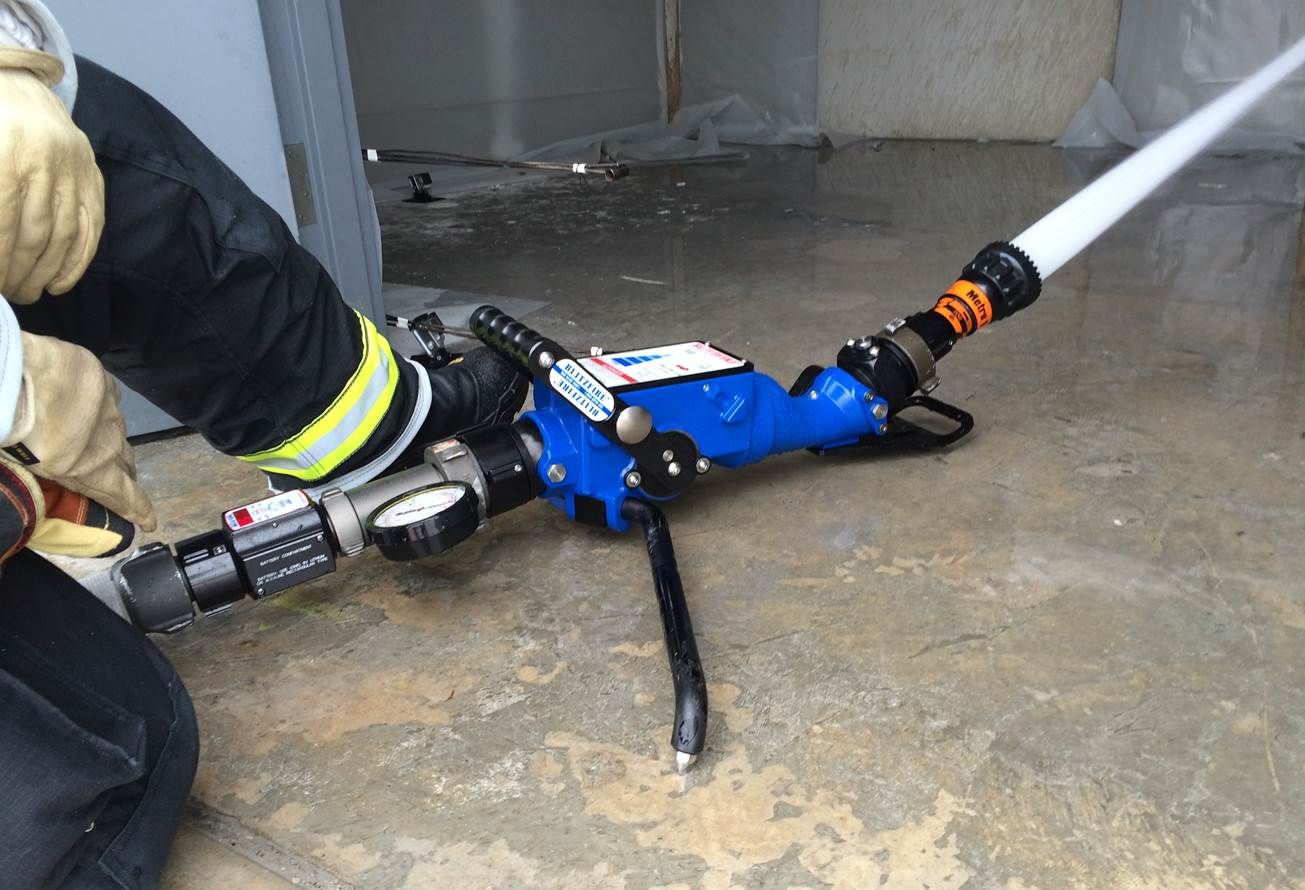
\includegraphics[width=2.9in]{../Figures/Pictures/monitor}
	\end{center} 
	\endminipage \hfill
	\minipage{3in}
	\begin{center}
		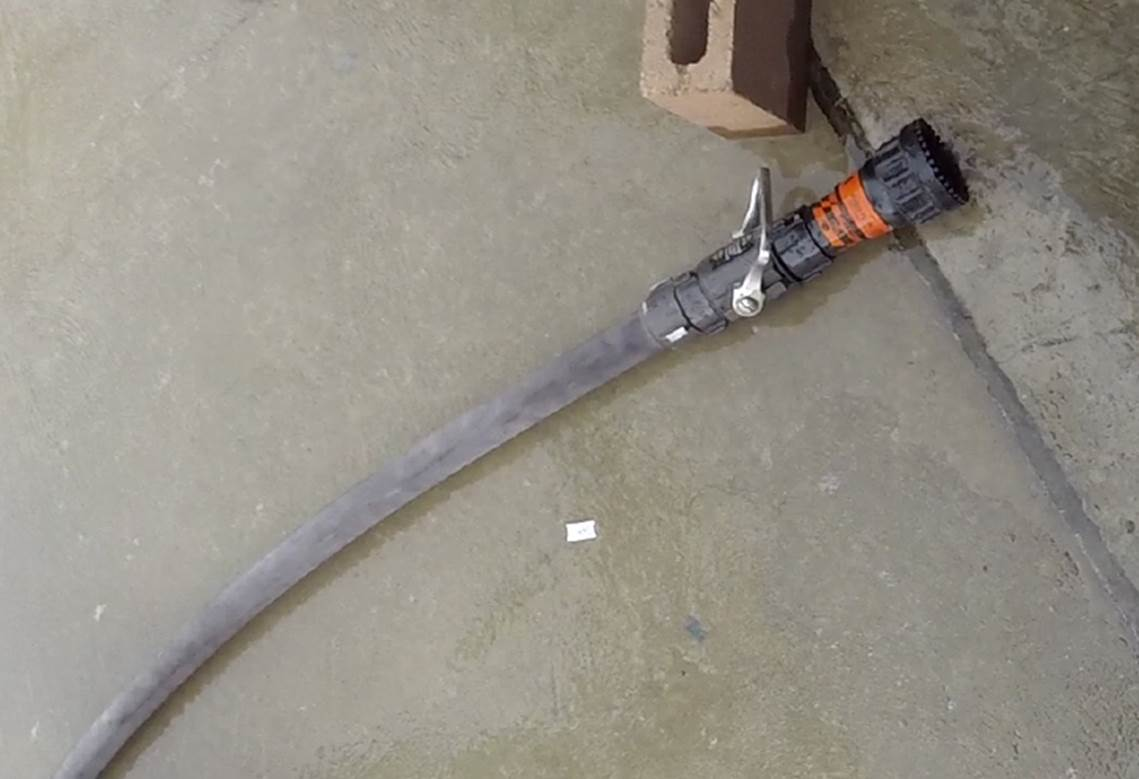
\includegraphics[width=2.9in]{../Figures/Pictures/handline}
	\end{center}
	\endminipage \hfill
	\caption[Monitor and handline equipped with a combination nozzle.]{Monitor (left) and 1.75~in handline (right) equipped with a combination nozzle and used to flow water during experiments.}
	\label{fig:monitor+handline}
\end{figure}

Three different structure flow path configurations were used for the seven experimental series. Tests~1 and 5 were conducted in the Single Story Structure and used a ``U-shaped'' configuration shown in Fig.~\ref{fig:east_setup}. Test~1 used a monitor and combination nozzle to flow water, and Test~5 used a combination nozzle attached directly to a handline to flow water.

Two different flow path configurations were used for the test series conducted in the Two Story Structure. The main difference between the two flow paths was the position of the south side door on the first level. Tests~2 and 6 used a configuration with the door opened (Fig.~\ref{fig:flow_path_1}), while Tests~3, 4, and 7 used a configuration with the door closed (Fig.~\ref{fig:flow_path_2}). Tests~2 and 3 used a combination nozzle attached to a monitor to flow water; Tests~6 and 7 used a combination nozzle attached directly to a handline to flow water; and Test~4 used both a combination nozzle and a 1~in tip smooth bore nozzle attached to a monitor to flow water in a straight and solid stream, respectively. 

\begin{figure}[!ht]
	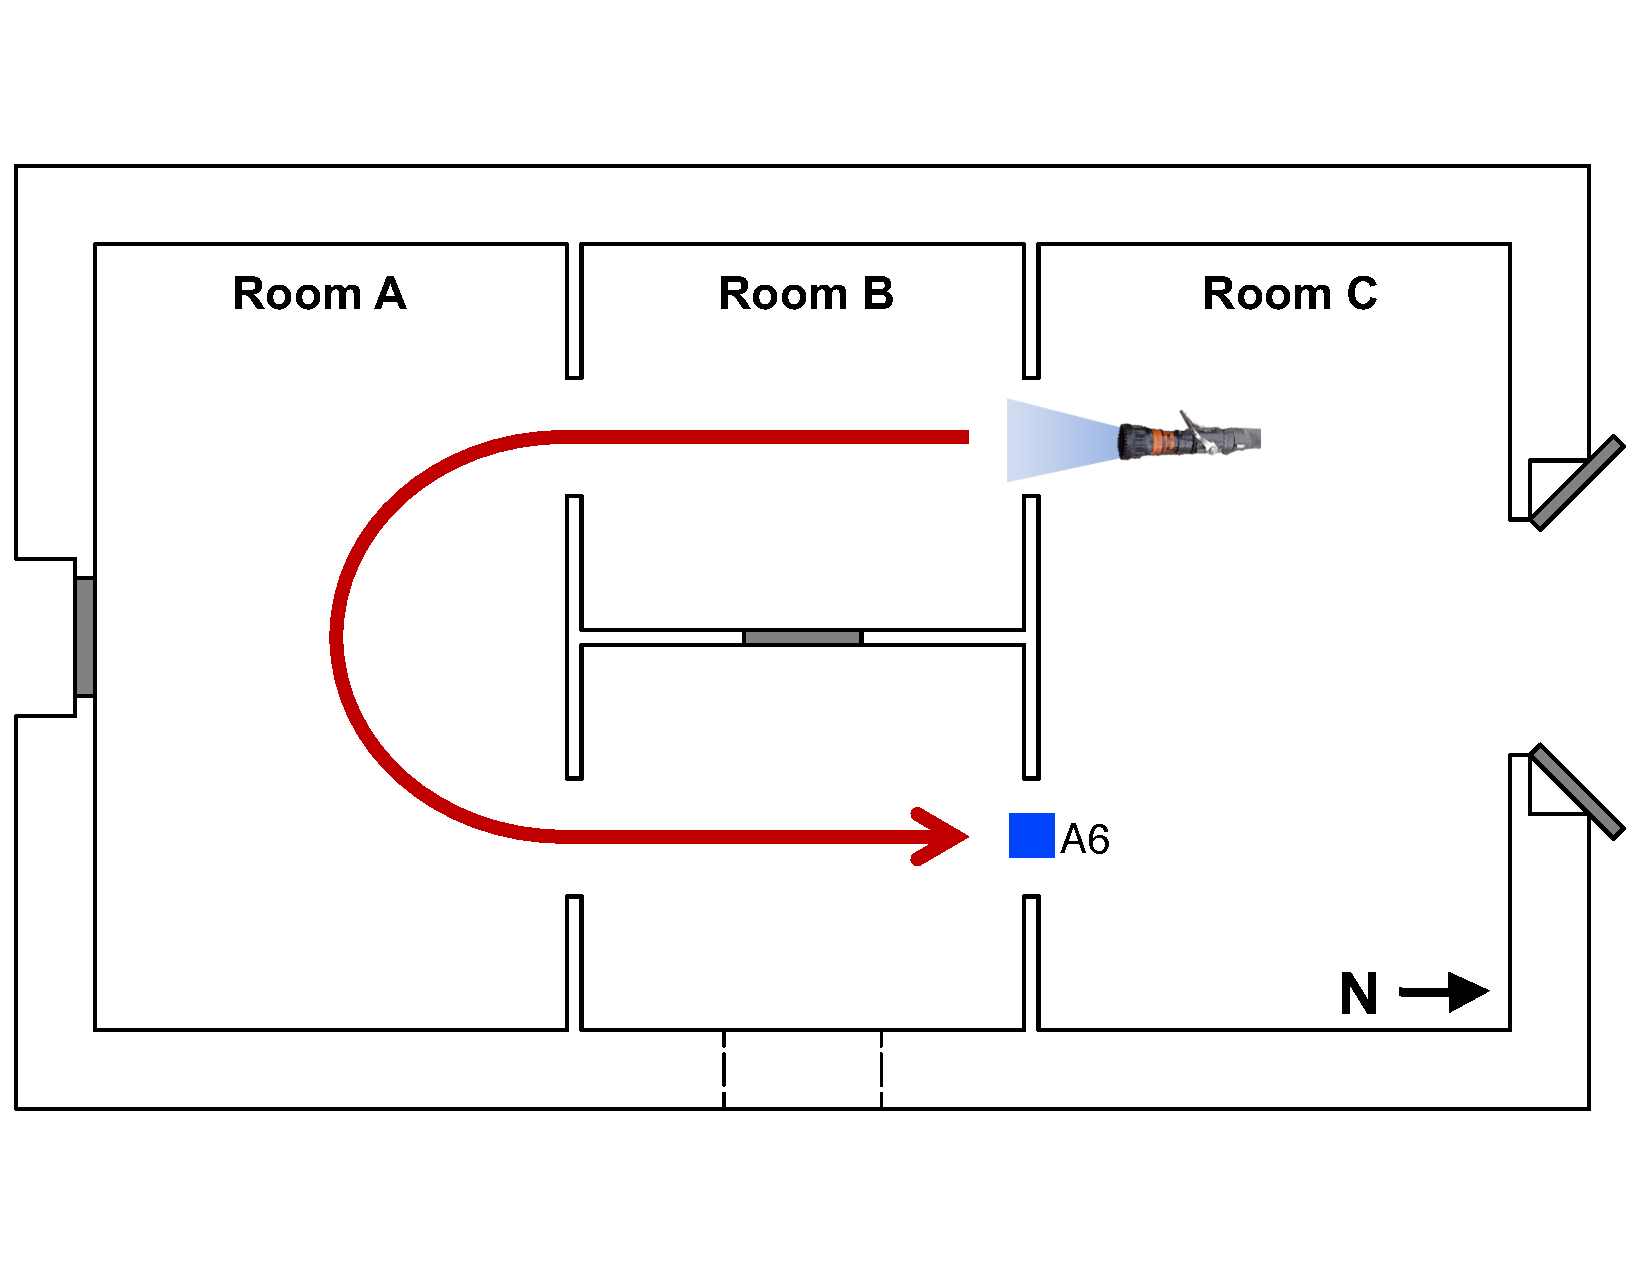
\includegraphics[width=\columnwidth]{../Figures/Floor_Plans/Specific_Tests/East_Hose_Test_Annotated}
	\caption[Plan view of the Single Story Structure setup for Tests~1 and 5.]{Plan view of the Single Story Structure setup for Tests~1 and 5. The view is annotated with the approximate location of water flow (nozzle graphic), the direction of the established flow path (red line), and the approximate location of bi-directional probe array A6 (blue square). The north side double doors remained opened for the entire duration of the experiments.}
	\label{fig:east_setup}
\end{figure}
\FloatBarrier

\begin{figure}[!ht]
	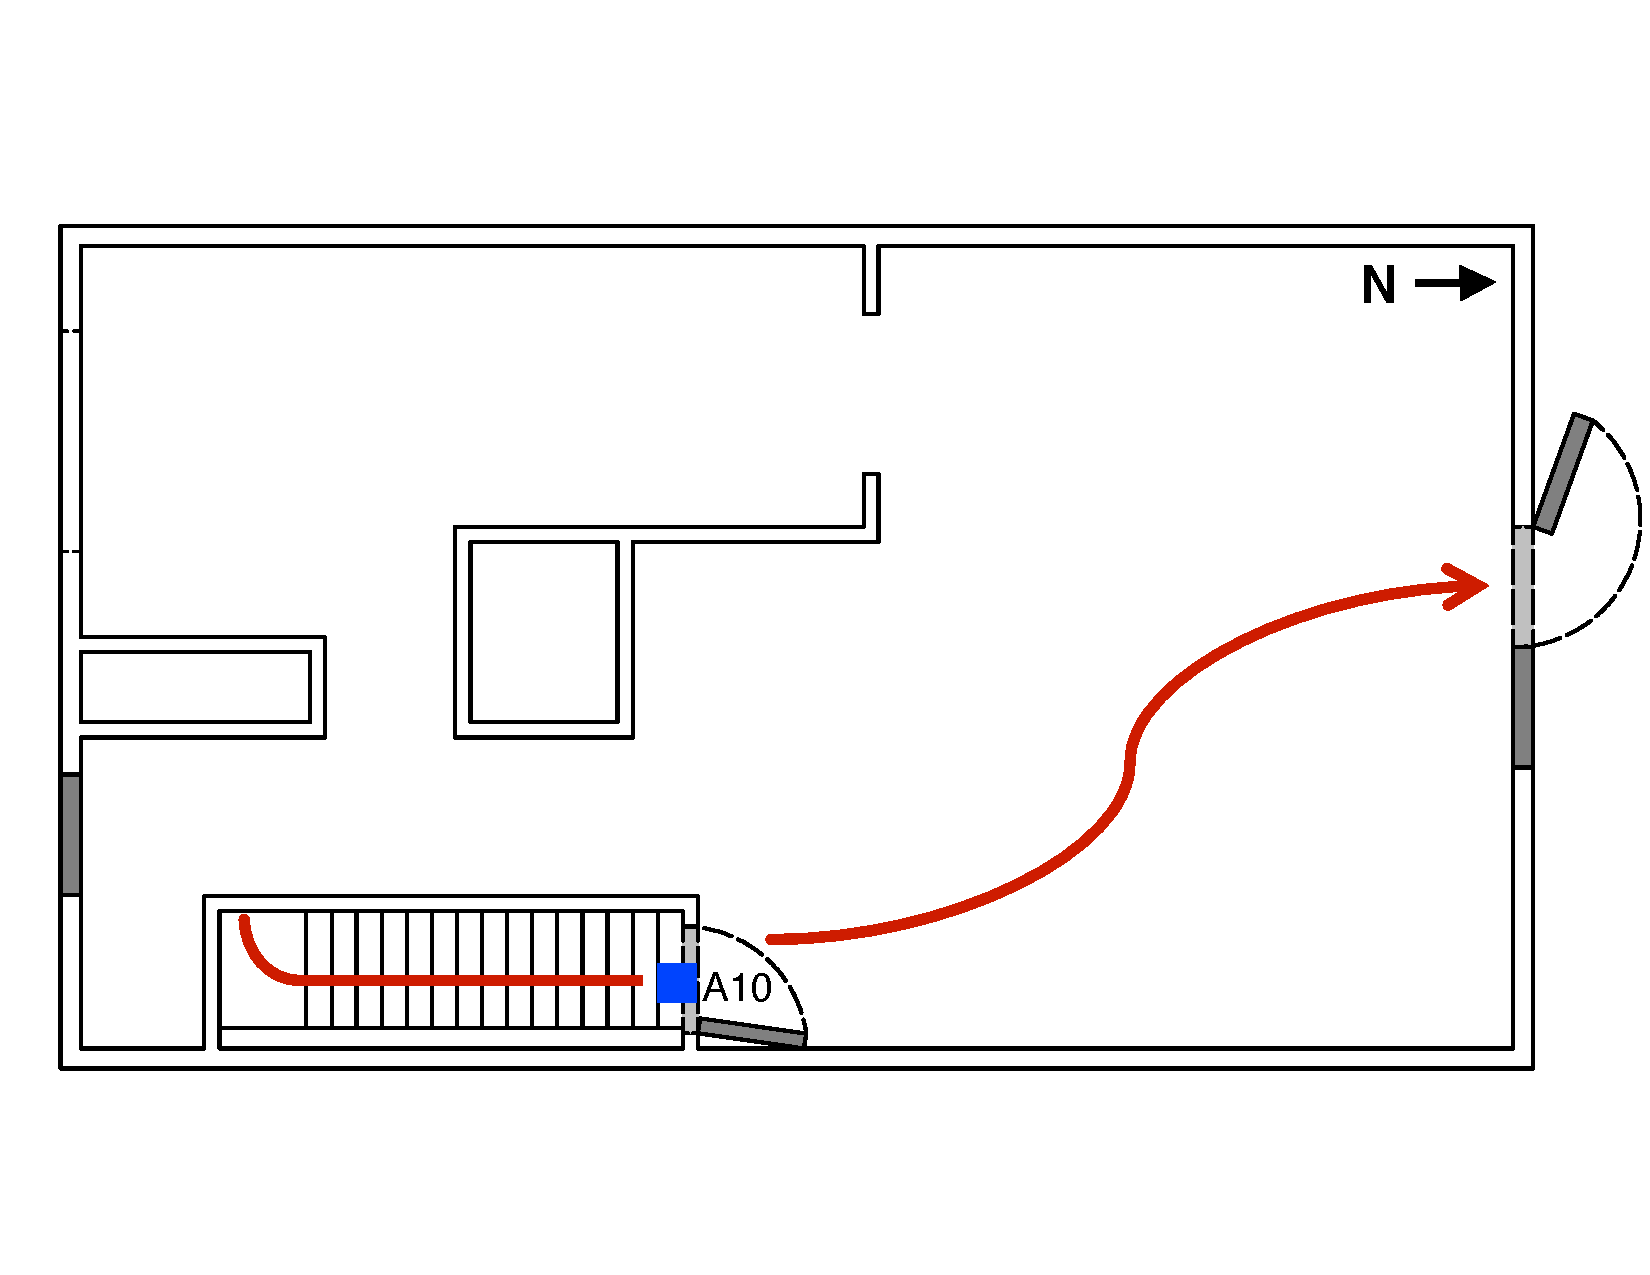
\includegraphics[width=\columnwidth]{../Figures/Floor_Plans/Specific_Tests/West_Hose_Test_2nd_Floor_Annotated}
	\\~\\
	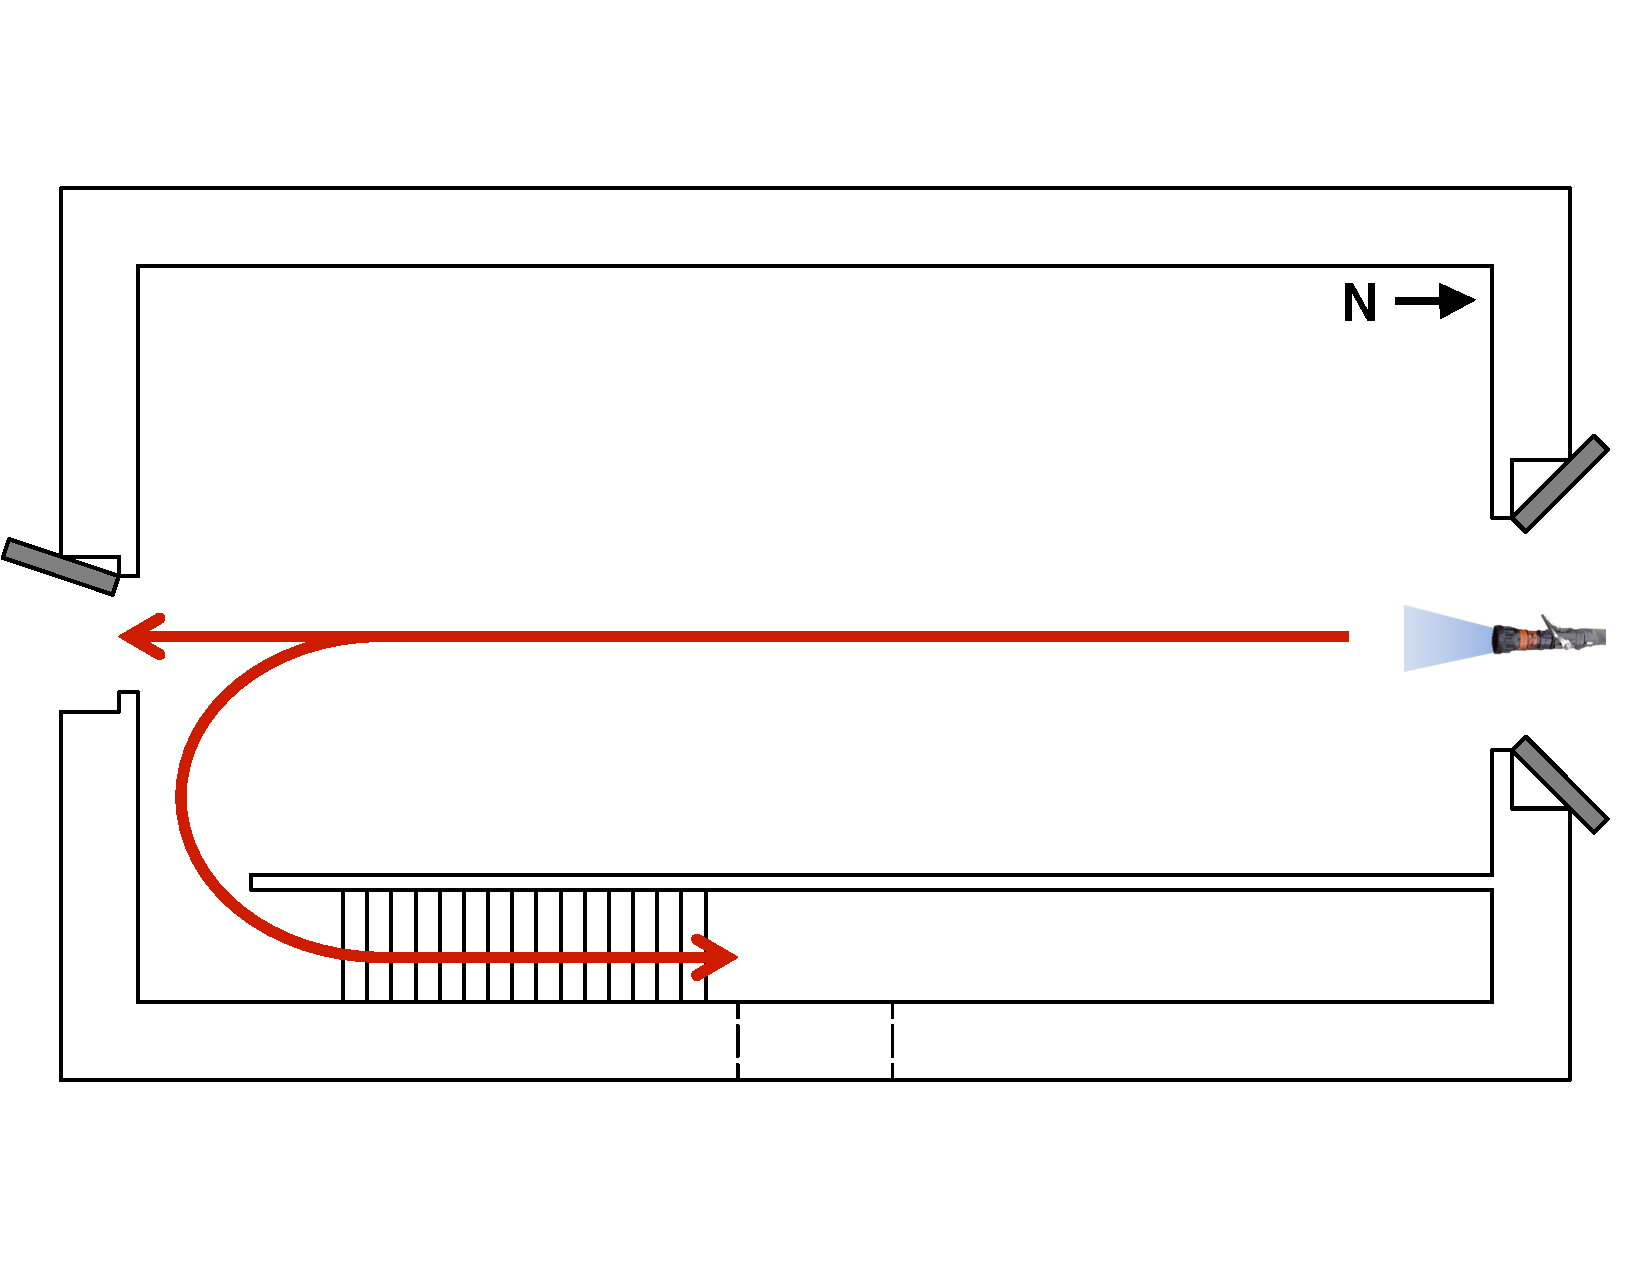
\includegraphics[width=\columnwidth]{../Figures/Floor_Plans/Specific_Tests/West_Hose_Test_18_1st_Floor_Annotated}
	\caption[Plan view of the Two Story Structure setup for Tests~2 and 6.]{Plan view of the second floor (top) and first floor (bottom) setup in the Two Story Structure for Tests~2 and 6. The view is annotated with the approximate location of water flow (nozzle graphic), the direction of the established flow path (red line), and the approximate location of bi-directional probe array A10 (blue square). The stairwell door and the west double door on the north side of the second floor were opened and closed at certain instances during the tests.}
	\label{fig:flow_path_1}
\end{figure}

\begin{figure}[!ht]
	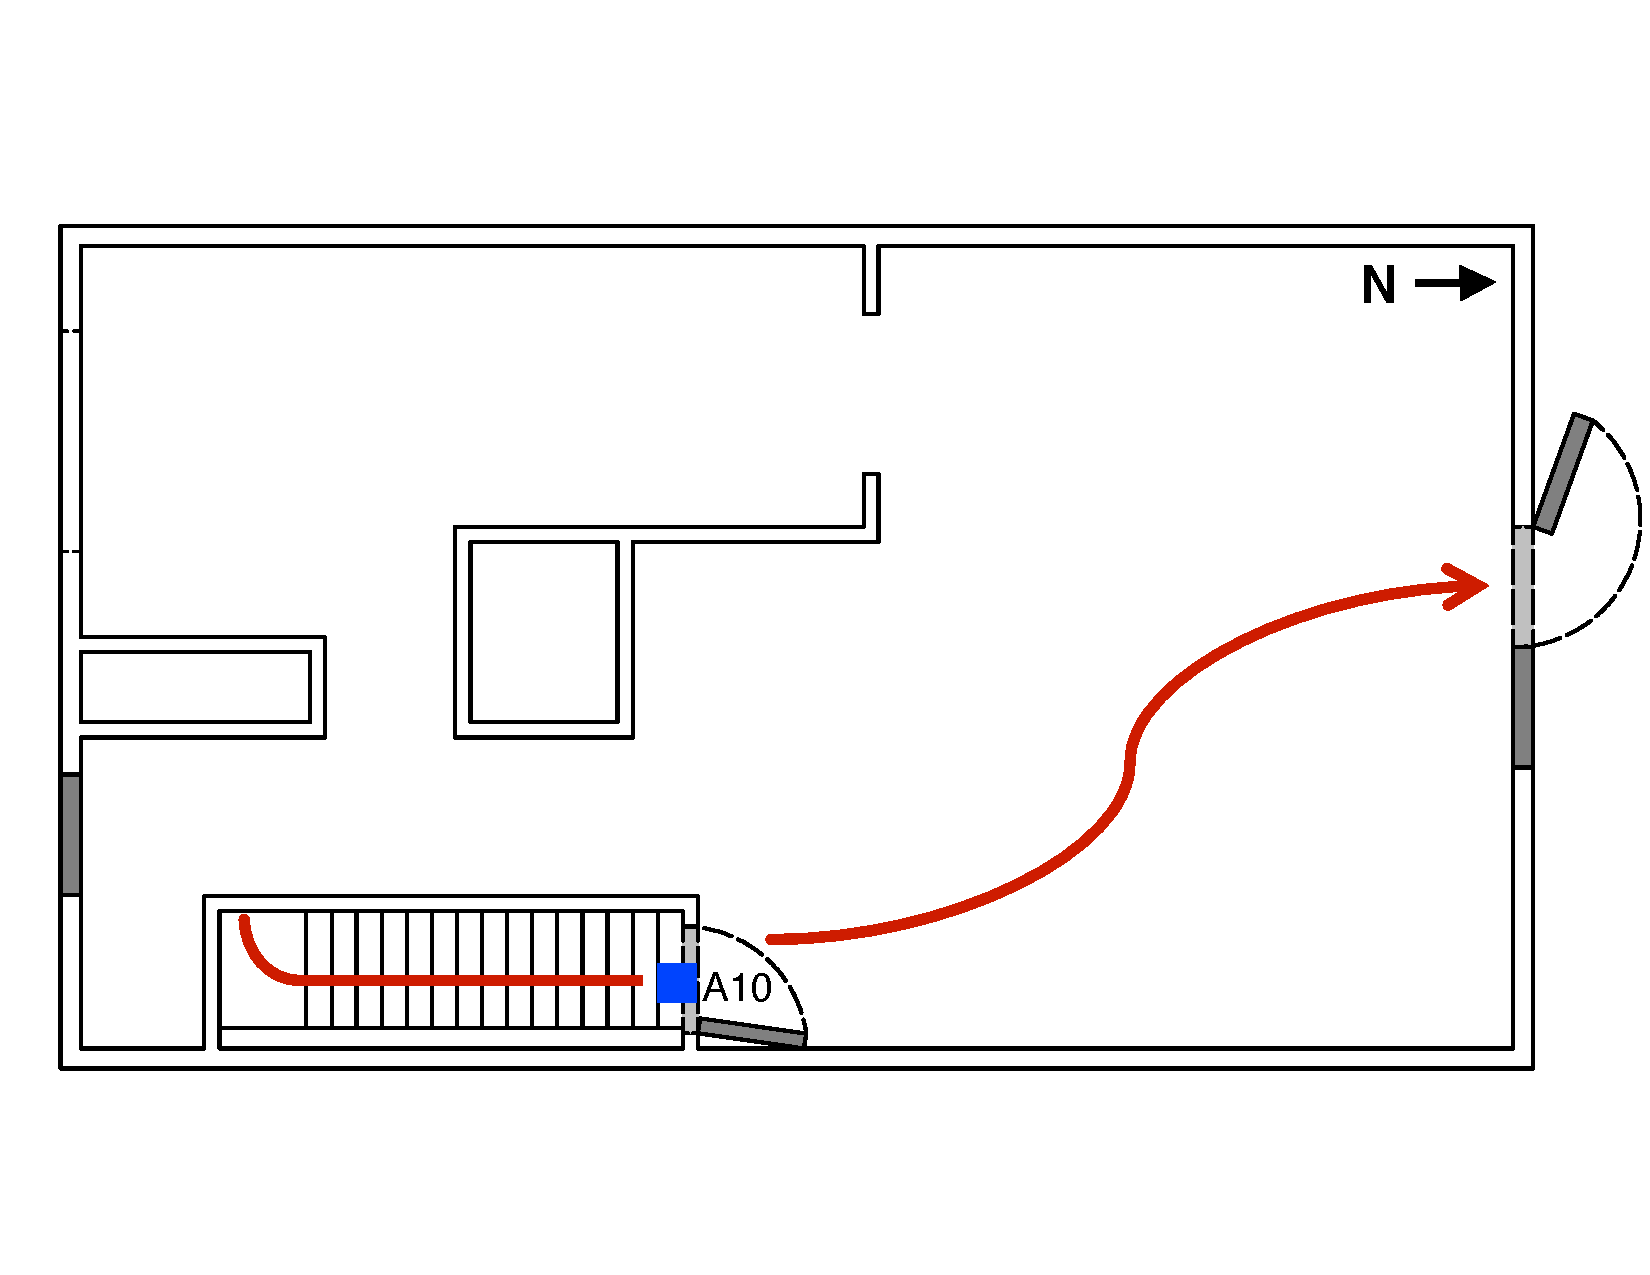
\includegraphics[width=\columnwidth]{../Figures/Floor_Plans/Specific_Tests/West_Hose_Test_2nd_Floor_Annotated}
	\\~\\
	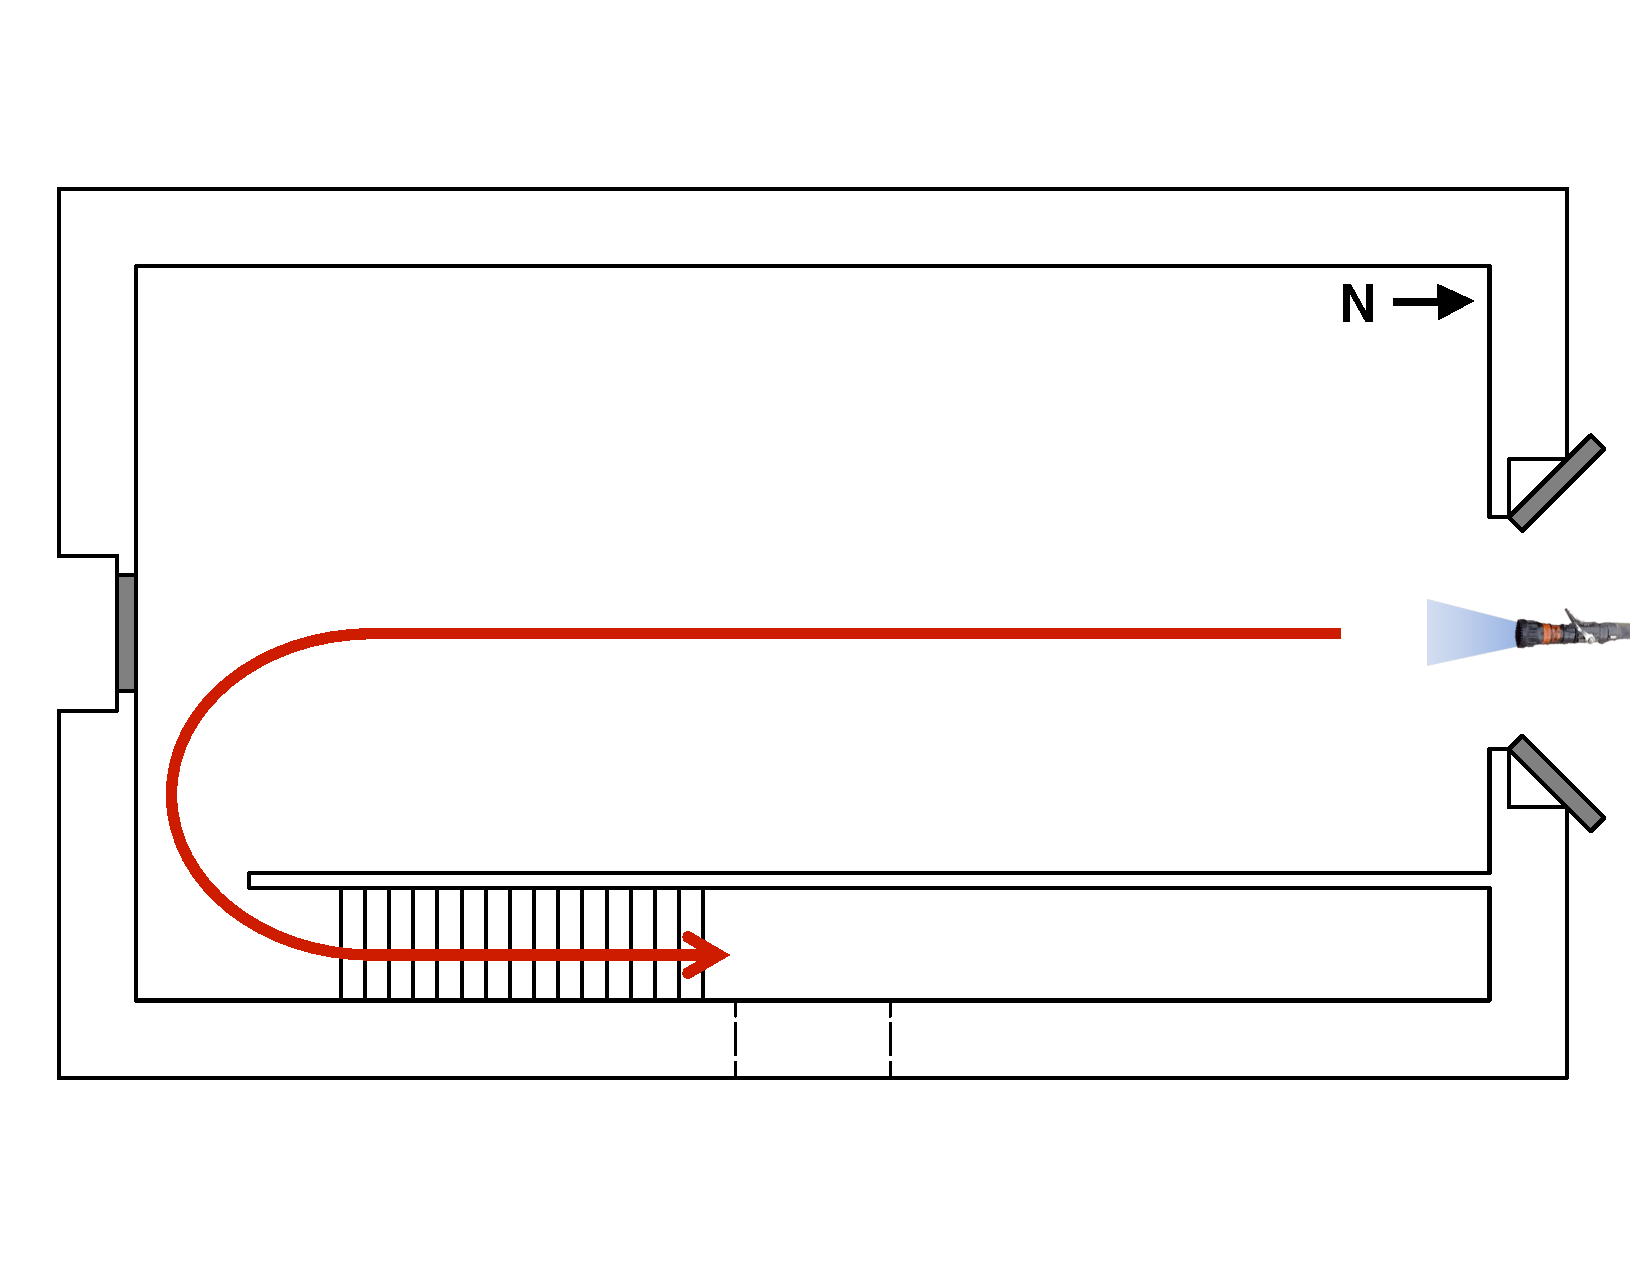
\includegraphics[width=\columnwidth]{../Figures/Floor_Plans/Specific_Tests/West_Hose_Test_19_1st_Floor_Annotated}
	\caption[Plan view of the Two Story Structure setup for Tests~3 and 7.]{Plan view of the second floor (top) and first floor (bottom) setup in the Two Story Structure for Tests~3, 4, and 7. The view is annotated with the approximate location of water flow (nozzle graphic), the direction of the established flow path (red line), and the approximate location of bi-directional probe array A10 (blue square). The stairwell door and the west double door on the north side of the second floor were opened and closed at certain instances during the tests.}
	\label{fig:flow_path_2}
\end{figure}
\FloatBarrier

\subsection{Monitor Experiments}
\label{sec:monitor_procedure}
Three experimental series, Tests~1--3, used a monitor equipped with a combination nozzle to flow water at 120~gpm in a straight stream, narrow fog stream, and wide fog stream. Test~1 occurred in the Single Story Structure, and Tests~2 and 3 occurred in the Two Story Structure. A fourth series, Test~4, was conducted in the Two Story Structure and used a combination nozzle and a smooth bore nozzle attached to a monitor to flow water at 180~gpm in a straight stream and solid stream, respectively. The monitor was always set to flow water from a fixed position. Thus, the monitor experiments primarily focused on the impact of different hose stream patterns on air movement in a structure and provided a baseline to compare the impact of the motion of the nozzle on the air movement through the structure.

\subsubsection{Test~1}
Test~1 utilized a monitor equipped with a combination nozzle to flow water from Room~C of the Single Story Structure to the area above the doorway on the south wall of Room~B (Fig.~\ref{fig:test_1_pic}). A plan view of the structure's layout during Test~1 can be found in Fig.~\ref{fig:east_setup}. The figure highlights the general direction of the established flow path along with the approximate location of A6, the bi-directional probe array used to measure gas velocity through the northeast interior doorway. The procedure for Test~1 was the simplest of all the test procedures. First, water was flowed in a straight stream for 30 seconds, then the stream was changed to a narrow fog for 30 seconds, and finally the stream was changed to a wide fog for 30 seconds. The procedure was repeated.

\begin{figure}[!ht]
	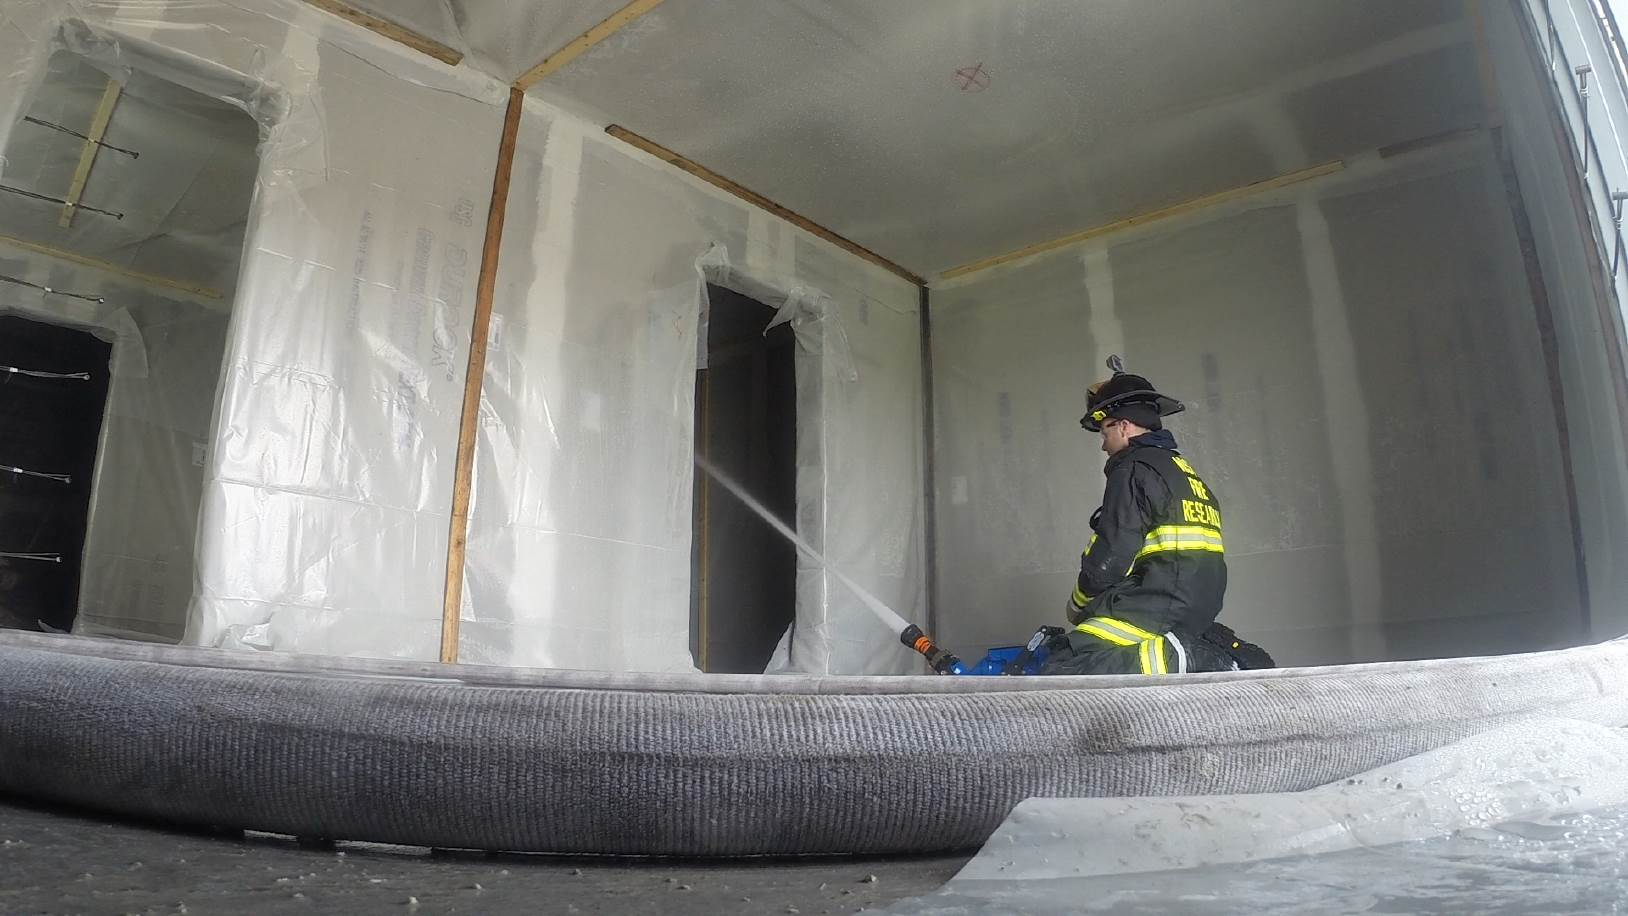
\includegraphics[trim=16cm 6.25cm 9cm 6cm, clip=true, width=4in]{../Figures/Pictures/SS_Room_B_Test_33}
	\\~\\
	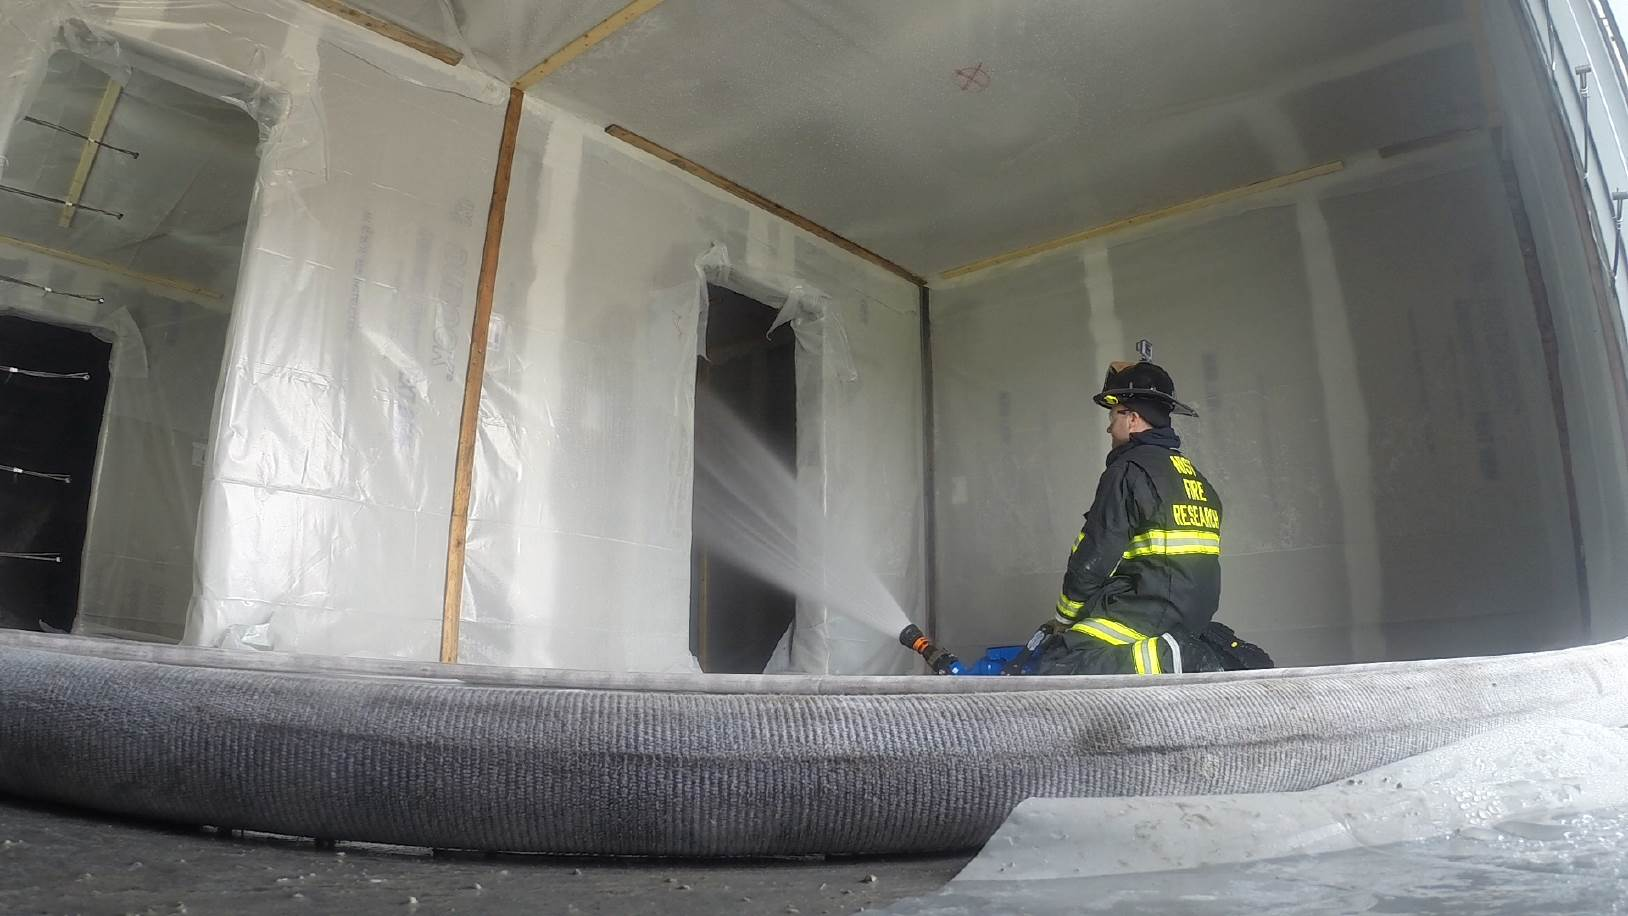
\includegraphics[trim=16cm 6.25cm 9cm 6cm, clip=true, width=4in]{../Figures/Pictures/NF_Room_B_Test_33}
	\\~\\
	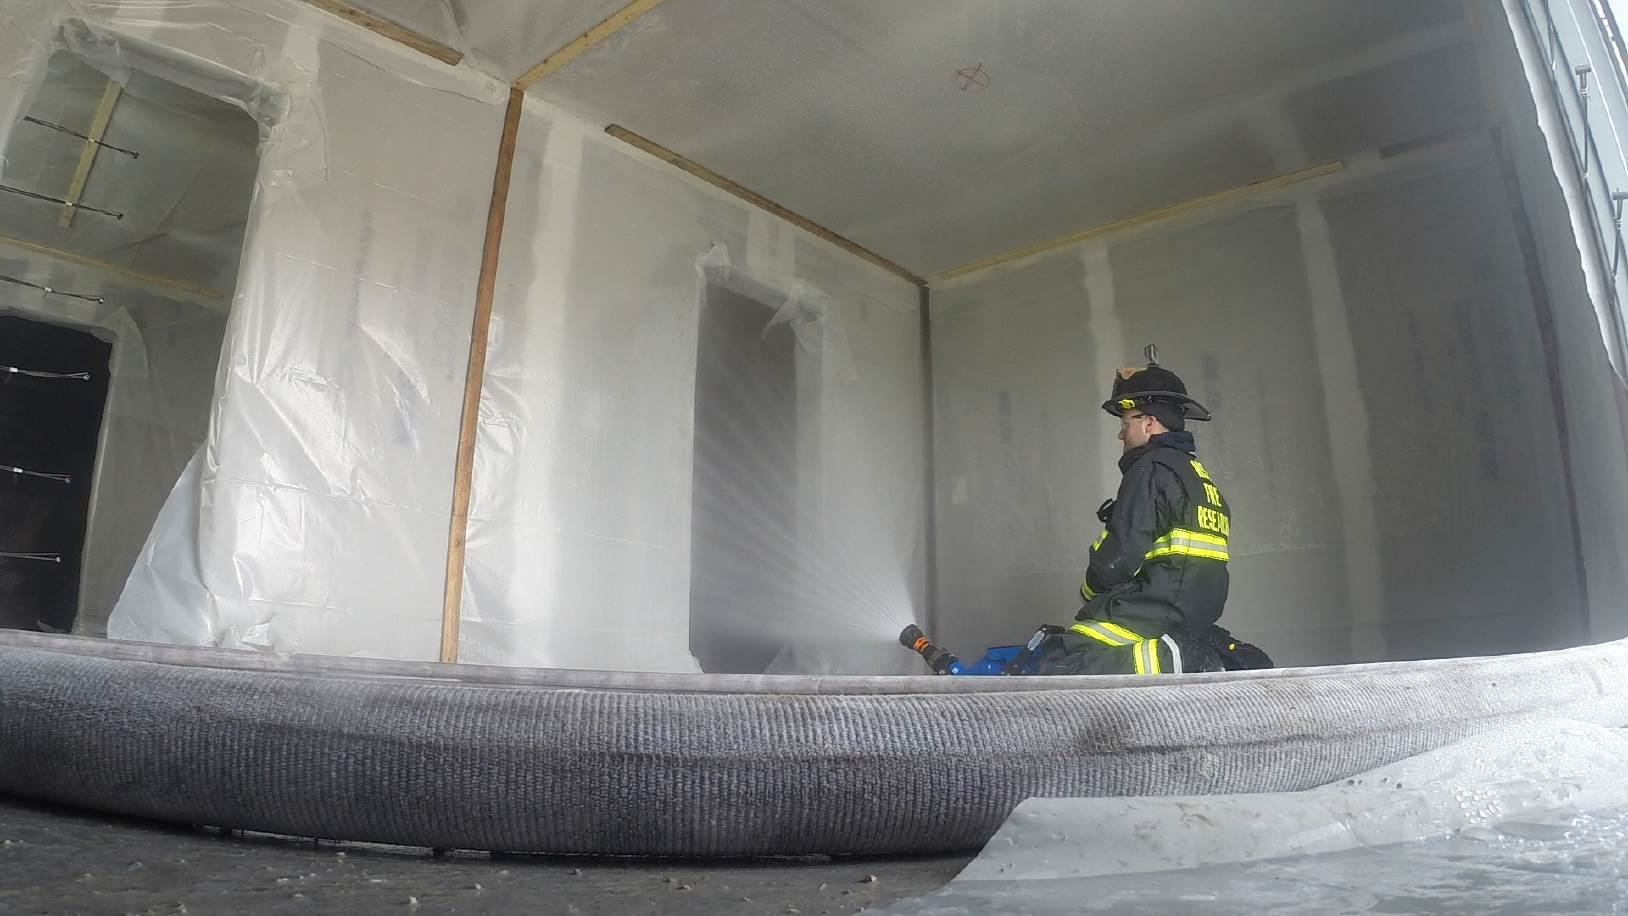
\includegraphics[trim=16cm 6.25cm 9cm 6cm, clip=true, width=4in]{../Figures/Pictures/WF_Room_B_Test_33}
	\caption[Straight stream, narrow fog stream, and wide fog stream during Test~1.]{Water flowing from the monitor in Room C in a straight stream (top), narrow fog stream (middle), and wide fog stream (bottom) aimed at the area above the doorway on the south wall of Room B during Test~1 in the Single Story Structure.}
	\label{fig:test_1_pic}
\end{figure}

\subsubsection{Tests~2 \& 3}
Tests~2 and 3 followed identical procedures that involved using a monitor equipped with a combination nozzle to flow water from the north side double doors to the interior ceiling on the first floor of the Two Story Structure. The nozzle was aimed at two regions marked on the center of the ceiling during the series: a ``near'' target located approximately 1.8~m (6~ft) from the interior side of the north wall and a ``far'' target located approximately 3.7~m (12~ft) from the interior side of the north wall. The procedure for each test began by flowing water in a straight stream pattern at the far target for 60 seconds. After 60 seconds of water flow, the stairwell door was opened. One minute later, the west double door on the north side of the second floor was opened, and water continued to flow for 60 seconds. Next, the water flow was stopped, the two doors were closed, and the procedure was repeated with the monitor aimed at the near target. This entire process was repeated using the narrow fog and wide fog streams. Fig.~\ref{fig:test_2_3_pic} contains images of each type of hose stream aimed at the near and far targets.

\begin{figure}[!ht]
	\minipage{2.15in}
	\begin{center}
		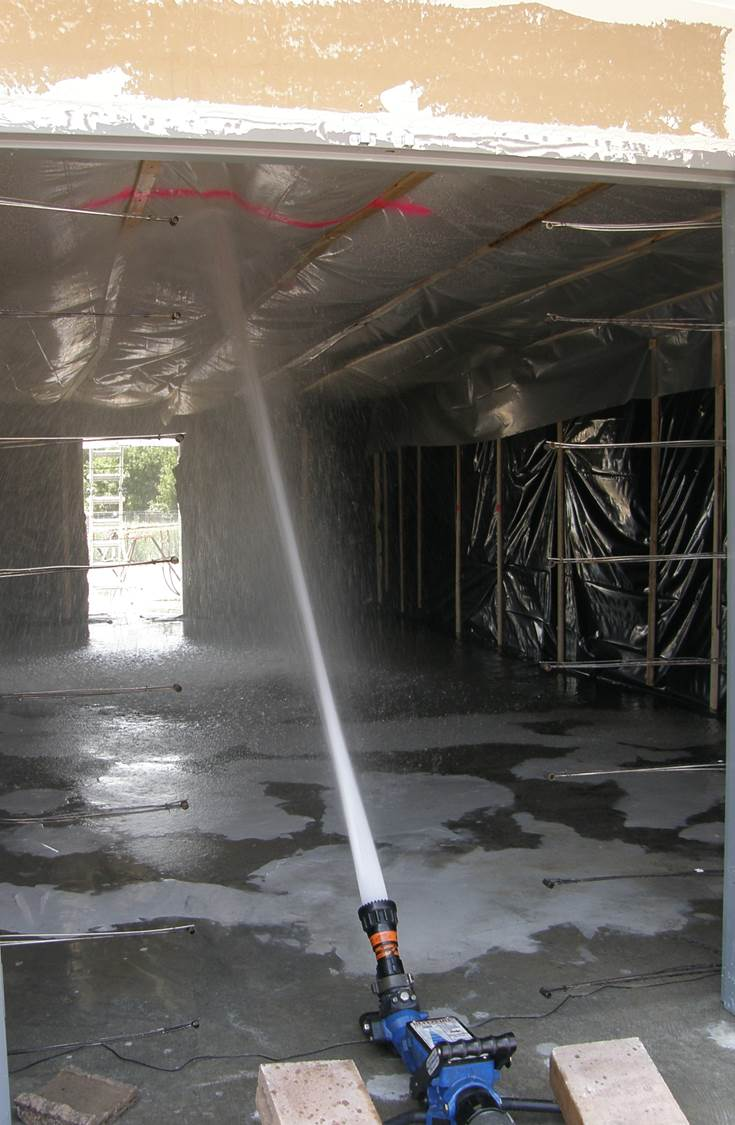
\includegraphics[width=2in]{../Figures/Pictures/SS_near}
	\end{center} 
	\endminipage \hfill
	\minipage{2.15in}
	\begin{center}
		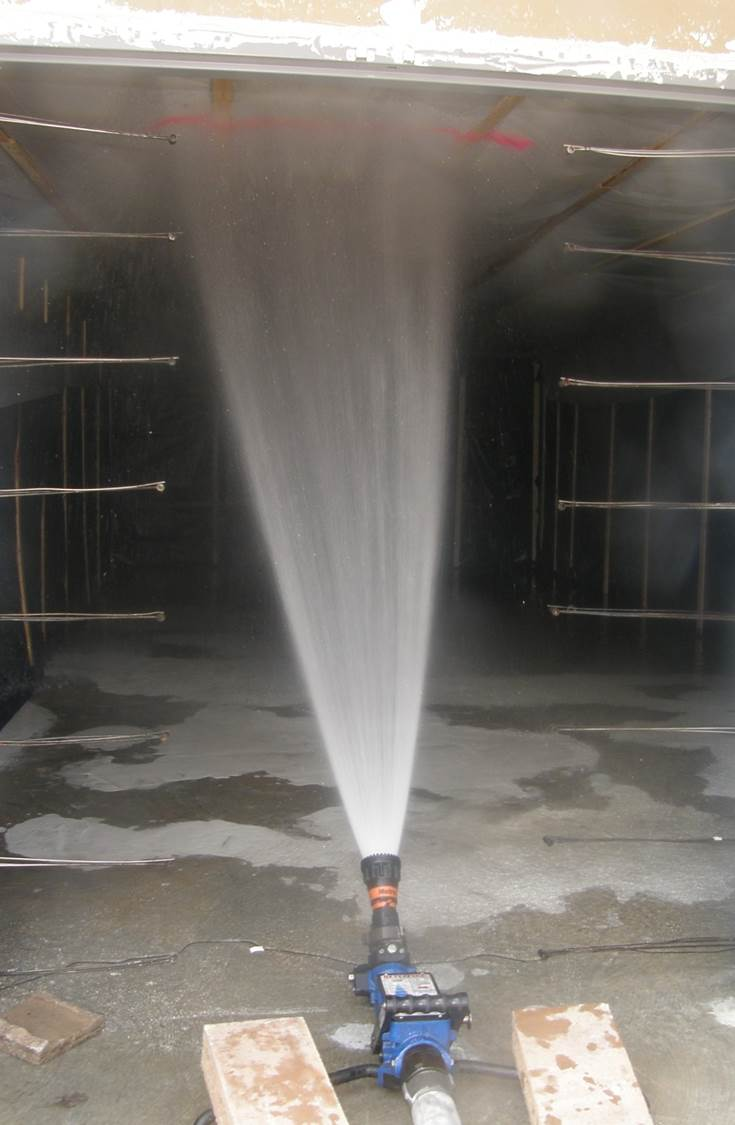
\includegraphics[width=2in]{../Figures/Pictures/NF_near}
	\end{center}
	\endminipage \hfill
	\minipage{2.15in}
	\begin{center}
		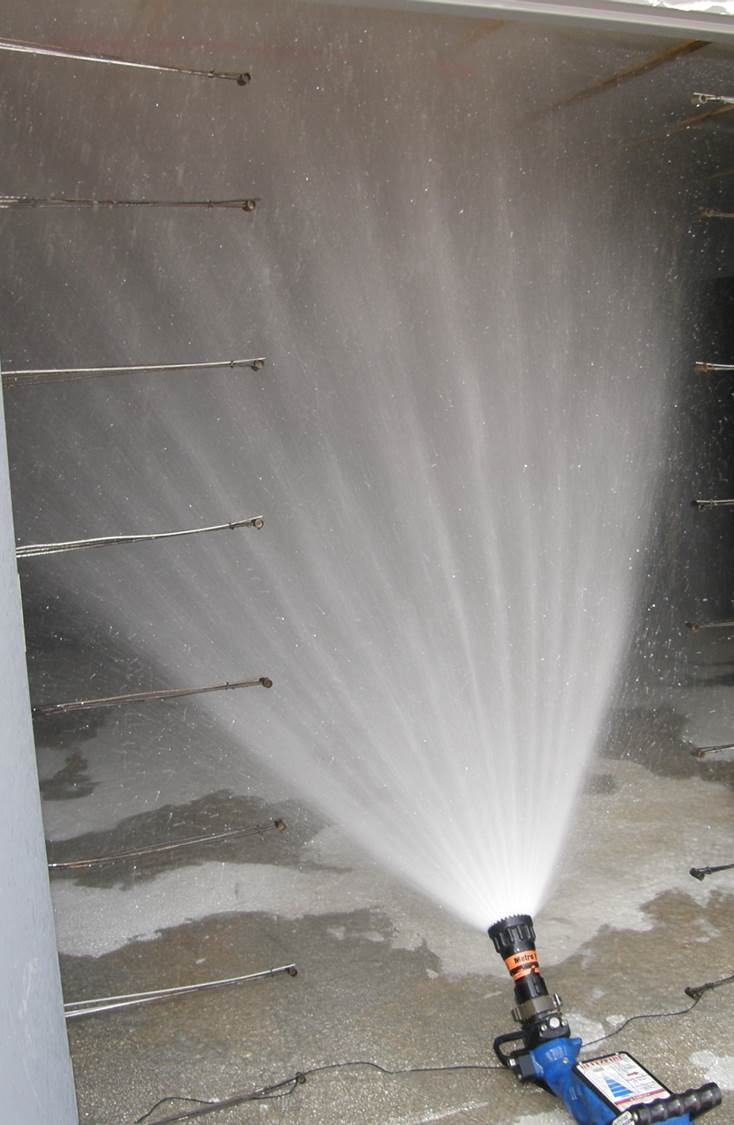
\includegraphics[width=2in]{../Figures/Pictures/WF_near}
	\end{center}
	\endminipage \hfill
	\vspace{0.15in}
	\minipage{2.15in}
	\begin{center}
		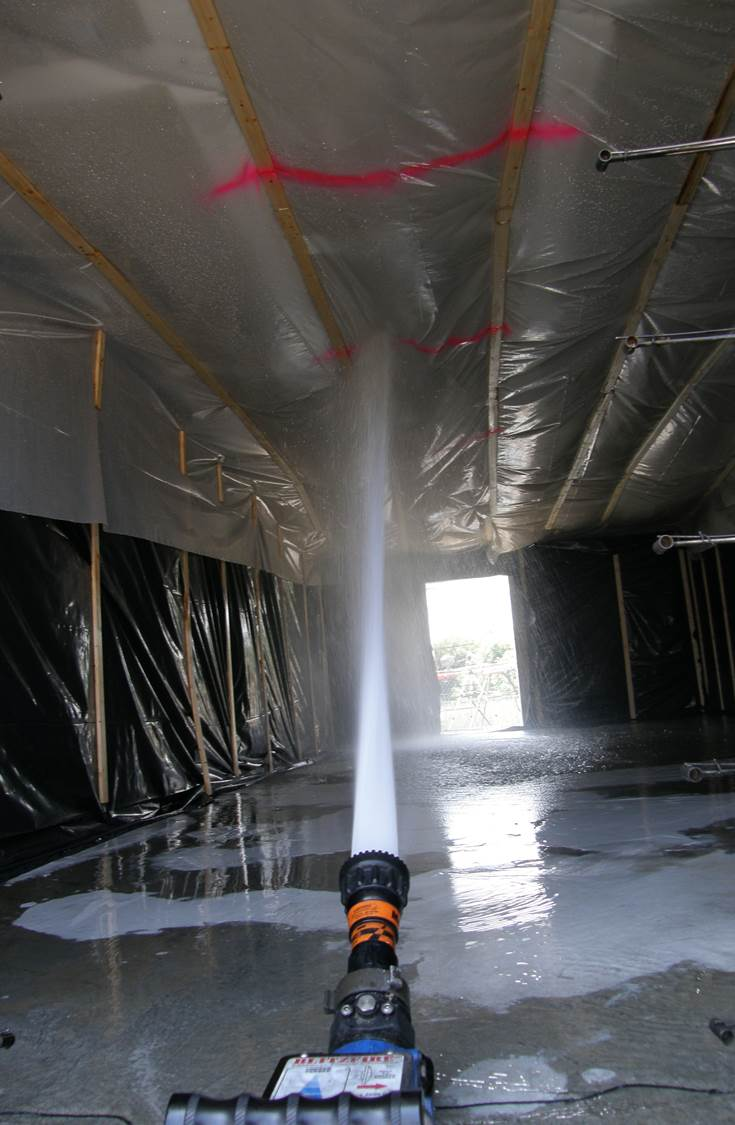
\includegraphics[width=2in]{../Figures/Pictures/SS_far}
	\end{center} 
	\endminipage \hfill
	\minipage{2.15in}
	\begin{center}
		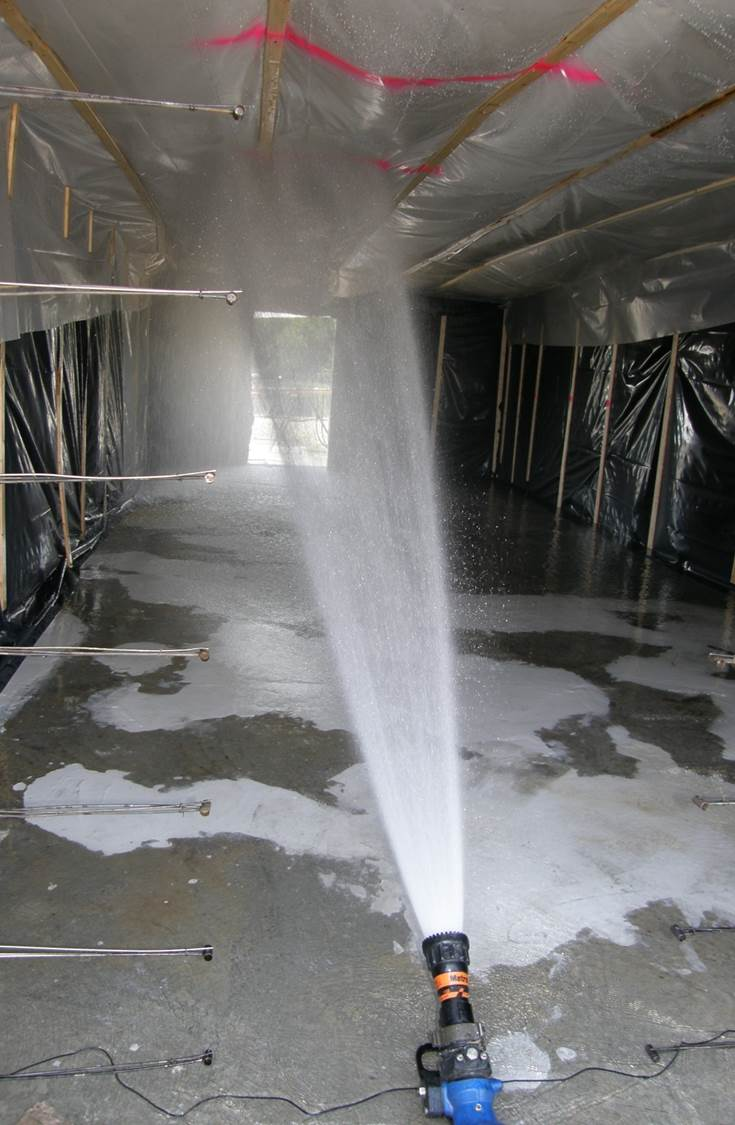
\includegraphics[width=2in]{../Figures/Pictures/NF_far}
	\end{center}
	\endminipage \hfill
	\minipage{2.15in}
	\begin{center}
		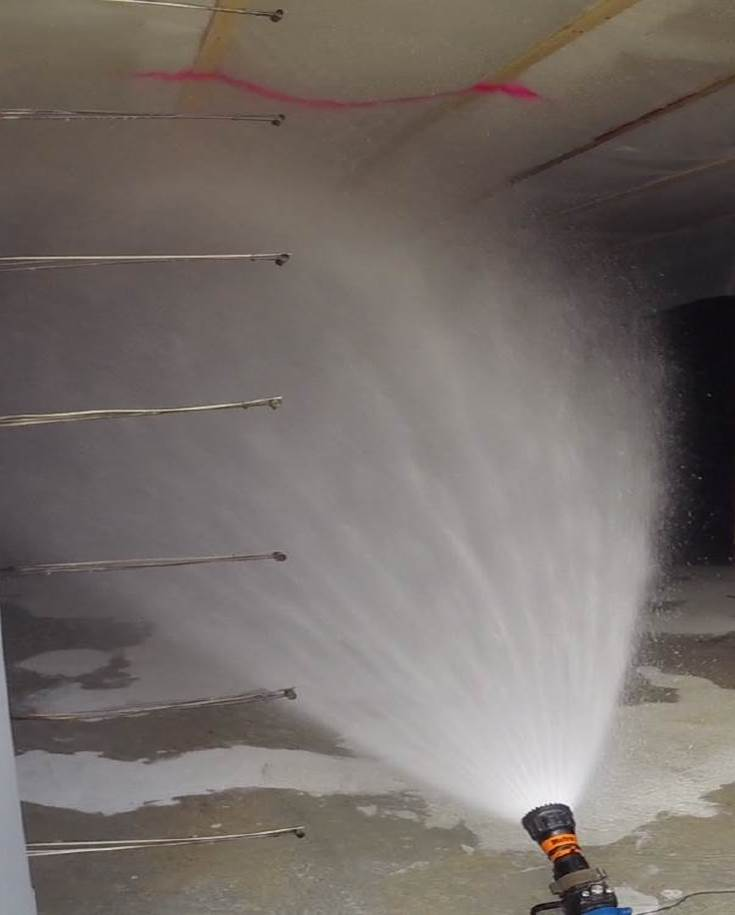
\includegraphics[width=2in]{../Figures/Pictures/WF_far}
	\end{center}
	\endminipage \hfill
	\caption[Straight stream, narrow fog stream, and wide fog stream aimed at the near and far targets in the Two Story Structure.]{Straight stream (left column), narrow fog stream (middle column), and wide fog stream (right column) aimed at ``near'' target (top row) and ``far'' target (bottom row) during Tests~2 and 3 in the Two Story Structure.}
	\label{fig:test_2_3_pic}
\end{figure}
\FloatBarrier

\subsubsection{Test~4}
Test~4 studied the differences in air movement caused by a solid stream from a smooth bore nozzle with a 1~in tip and straight stream from a combination nozzle attached to a monitor aimed at the same targets used during Tests~2 and 3. The stairwell door was opened for the entire experimental series. The test began by flowing water in a straight stream from a combination nozzle aimed at the near target. Then, the west double door on the second floor was opened. After 60 more seconds of flow, the nozzle was closed to stop water flow for 30 seconds. The nozzle was opened for 60 seconds and then closed for 30 seconds two additional times. Next, the monitor was aimed at the far target, and the procedure was repeated. This entire process was repeated for the solid stream from the smooth bore nozzle. Fig.~\ref{fig:test_4_pic} contains images of the straight stream from the combination nozzle and solid stream from the 1~in tip of the smooth bore nozzle during Test~4.

\begin{figure}[!ht]
	\minipage{2.15in}
	\begin{center}
		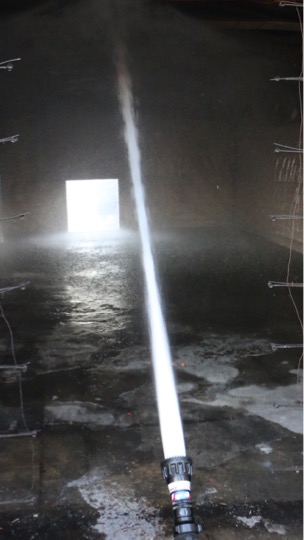
\includegraphics[width=2in]{../Figures/Pictures/SS_70}
	\end{center} 
	\endminipage
	\minipage{2.15in}
	\begin{center}
		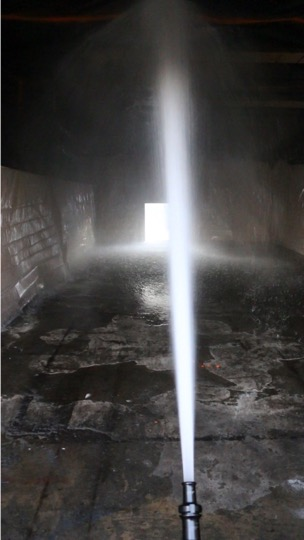
\includegraphics[width=2in]{../Figures/Pictures/SB_70}
	\end{center}
	\endminipage
	\caption[Straight stream from combination nozzle and solid stream from smooth bore nozzle with 1~in tip during Test~4.]{Straight stream flowing from the combination nozzle (left) and solid stream flowing from the smooth bore nozzle (right) during Test~4.}
	\label{fig:test_4_pic}
\end{figure}
\FloatBarrier

\subsection{Handline Experiments}
\label{sec:handline_procedure}
Three experimental series were conducted using a 1.75~in handline with a combination nozzle to flow water in a straight stream, narrow fog stream, and wide fog stream. One series, Test~5, occurred in the Single Story Structure, and the remaining tests, Tests~6 and 7, occurred in the Two Story Structure. All three tests primarily focused on the impact of different hose stream and nozzle motion pattern selections on air movement in a structure. 

\subsubsection{Test~5}
Test~5 utilized a 1.75~in handline equipped with a combination nozzle to flow water from Room C of the Single Story Structure into Room B (Fig.~\ref{fig:test_5_pic}). The layout of the structure was identical to the layout for Test~1, described above in Section~\ref{sec:monitor_procedure} and presented in Fig.~\ref{fig:east_setup}. The procedure for Test~5 began by flowing water in a straight stream aimed at the ceiling of Room B for 30 seconds in a fixed position. After 30 seconds, the nozzle was rotated in the clockwise direction for 30 seconds. Then, the nozzle was aimed at the south doorway of Room B, and water was applied for 30 seconds in a fixed position followed by 30 seconds in a clockwise pattern. The procedure was repeated using a narrow fog stream and a wide fog stream. This entire process was repeated for the streams being applied in the fixed and counterclockwise patterns.

\begin{figure}[!ht]
	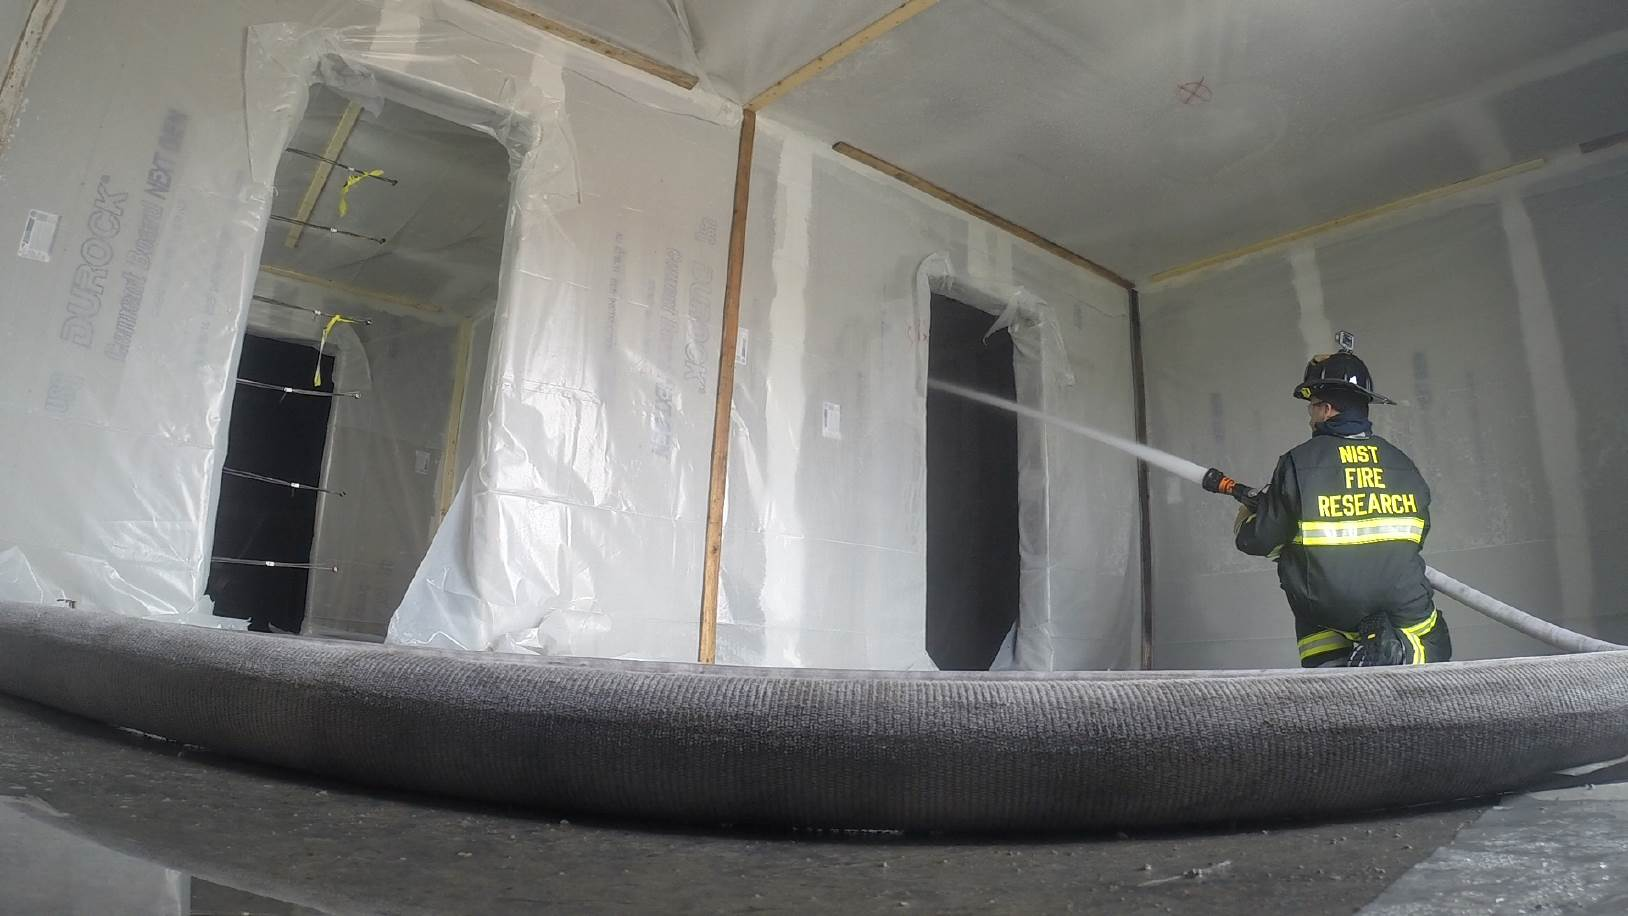
\includegraphics[trim=23cm 6.5cm 4cm 6cm, clip=true, width=3.75in]{../Figures/Pictures/SS_Room_B_Test_34}
	\\~\\
	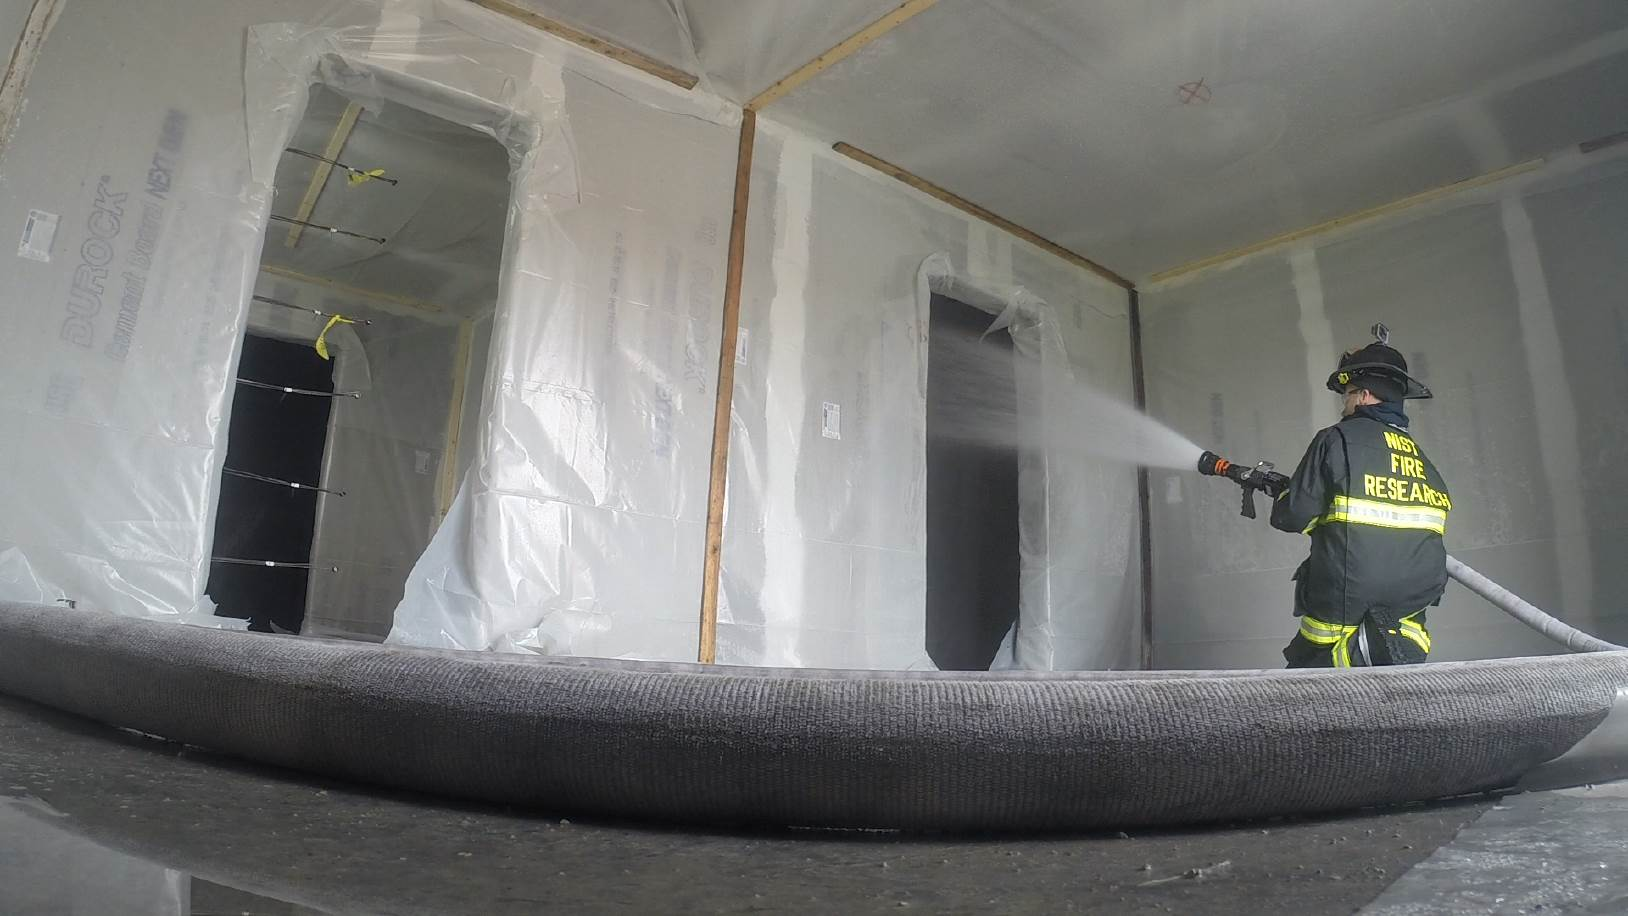
\includegraphics[trim=23cm 6.5cm 4cm 6cm, clip=true, width=3.75in]{../Figures/Pictures/NF_Room_B_Test_34}
	\\~\\
	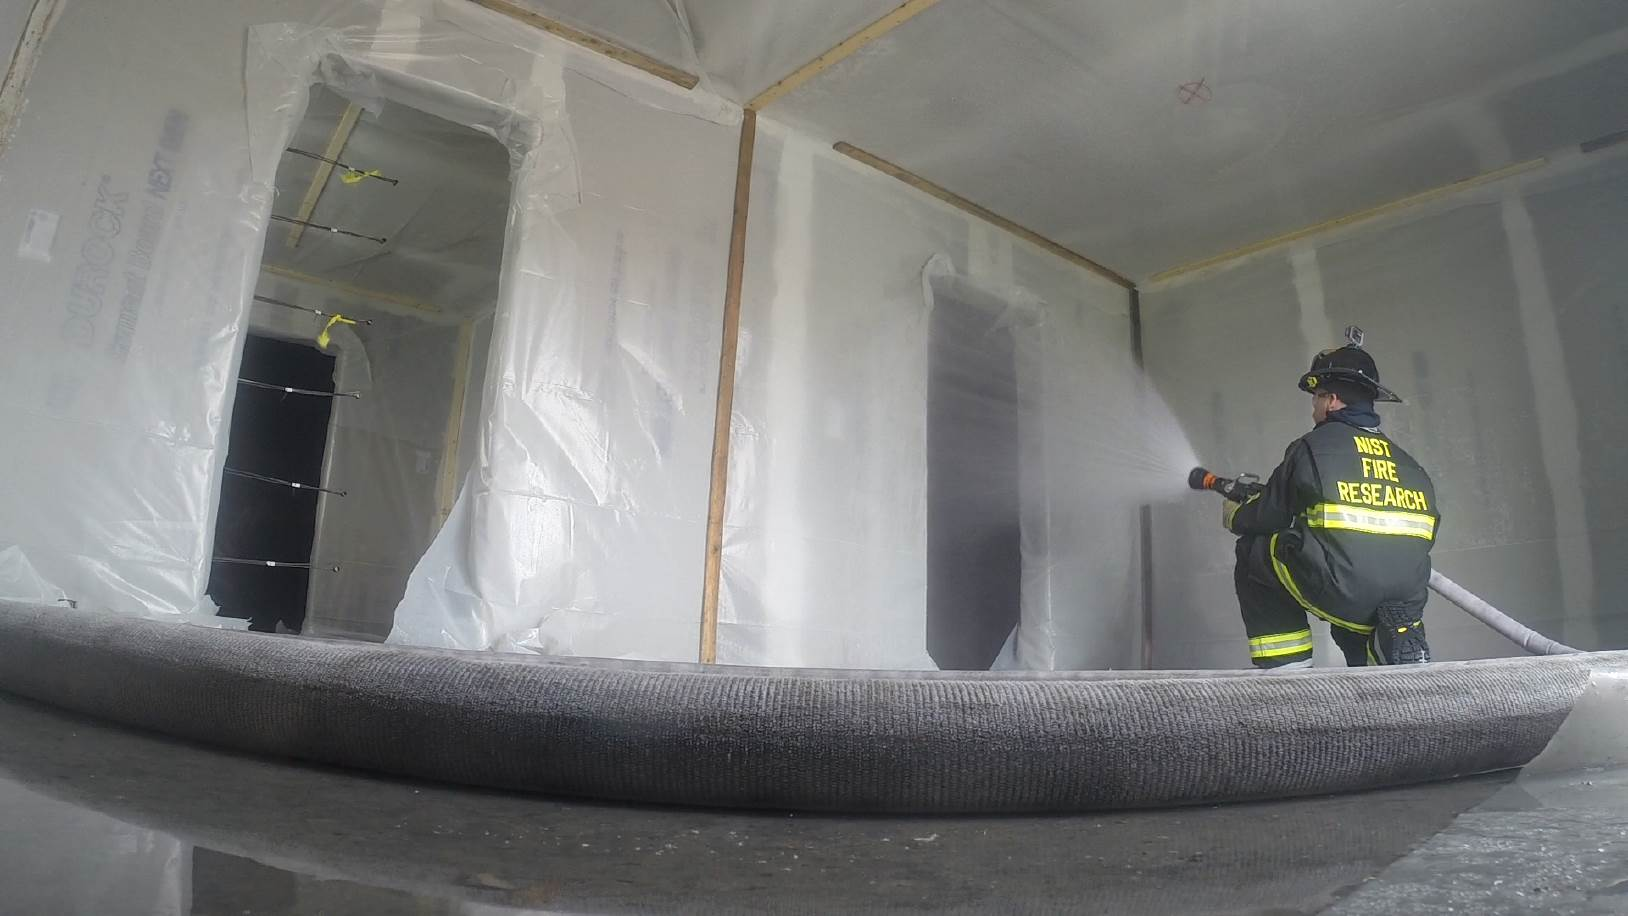
\includegraphics[trim=23cm 6.5cm 4cm 6cm, clip=true, width=3.75in]{../Figures/Pictures/WF_Room_B_Test_34}
	\caption[Straight stream, narrow fog stream, and wide fog stream during Test~5.]{Straight stream (top), narrow fog stream (middle), and wide fog stream (bottom) aimed at the south doorway of Room B during Test~5.}
	\label{fig:test_5_pic}
\end{figure}

\subsubsection{Tests~6 \& 7}
Tests~6 and 7 followed identical procedures that involved using a 1.75~in handline equipped with a combination nozzle to flow water from the north side double doors of the Two Story Structure into the first floor room. The water stream was aimed at the south side wall of the first floor during the experiments. Test~6 contained the flow path configuration presented in Fig.~\ref{fig:flow_path_1}, and Test~7 contained the flow path configuration presented in Fig.~\ref{fig:flow_path_2}. Each test began by using a straight stream to flow water in a fixed, horizontal position. After 60 seconds of water flow, the stairwell door was opened. One minute later, the west double door on the north side of the second floor was opened, and water continued to flow for 60 seconds. Next, the water flow was stopped, the two doors were closed, and the procedure was repeated three additional times for the sweeping (back and forth, left-to-right), clockwise, and counterclockwise nozzle motion patterns. This entire process was repeated using narrow fog and wide fog streams. Fig.~\ref{fig:test_6_pic} contains an image of a straight stream pattern being applied during Test~6 with the flow path fully established.

\begin{figure}[!ht]
	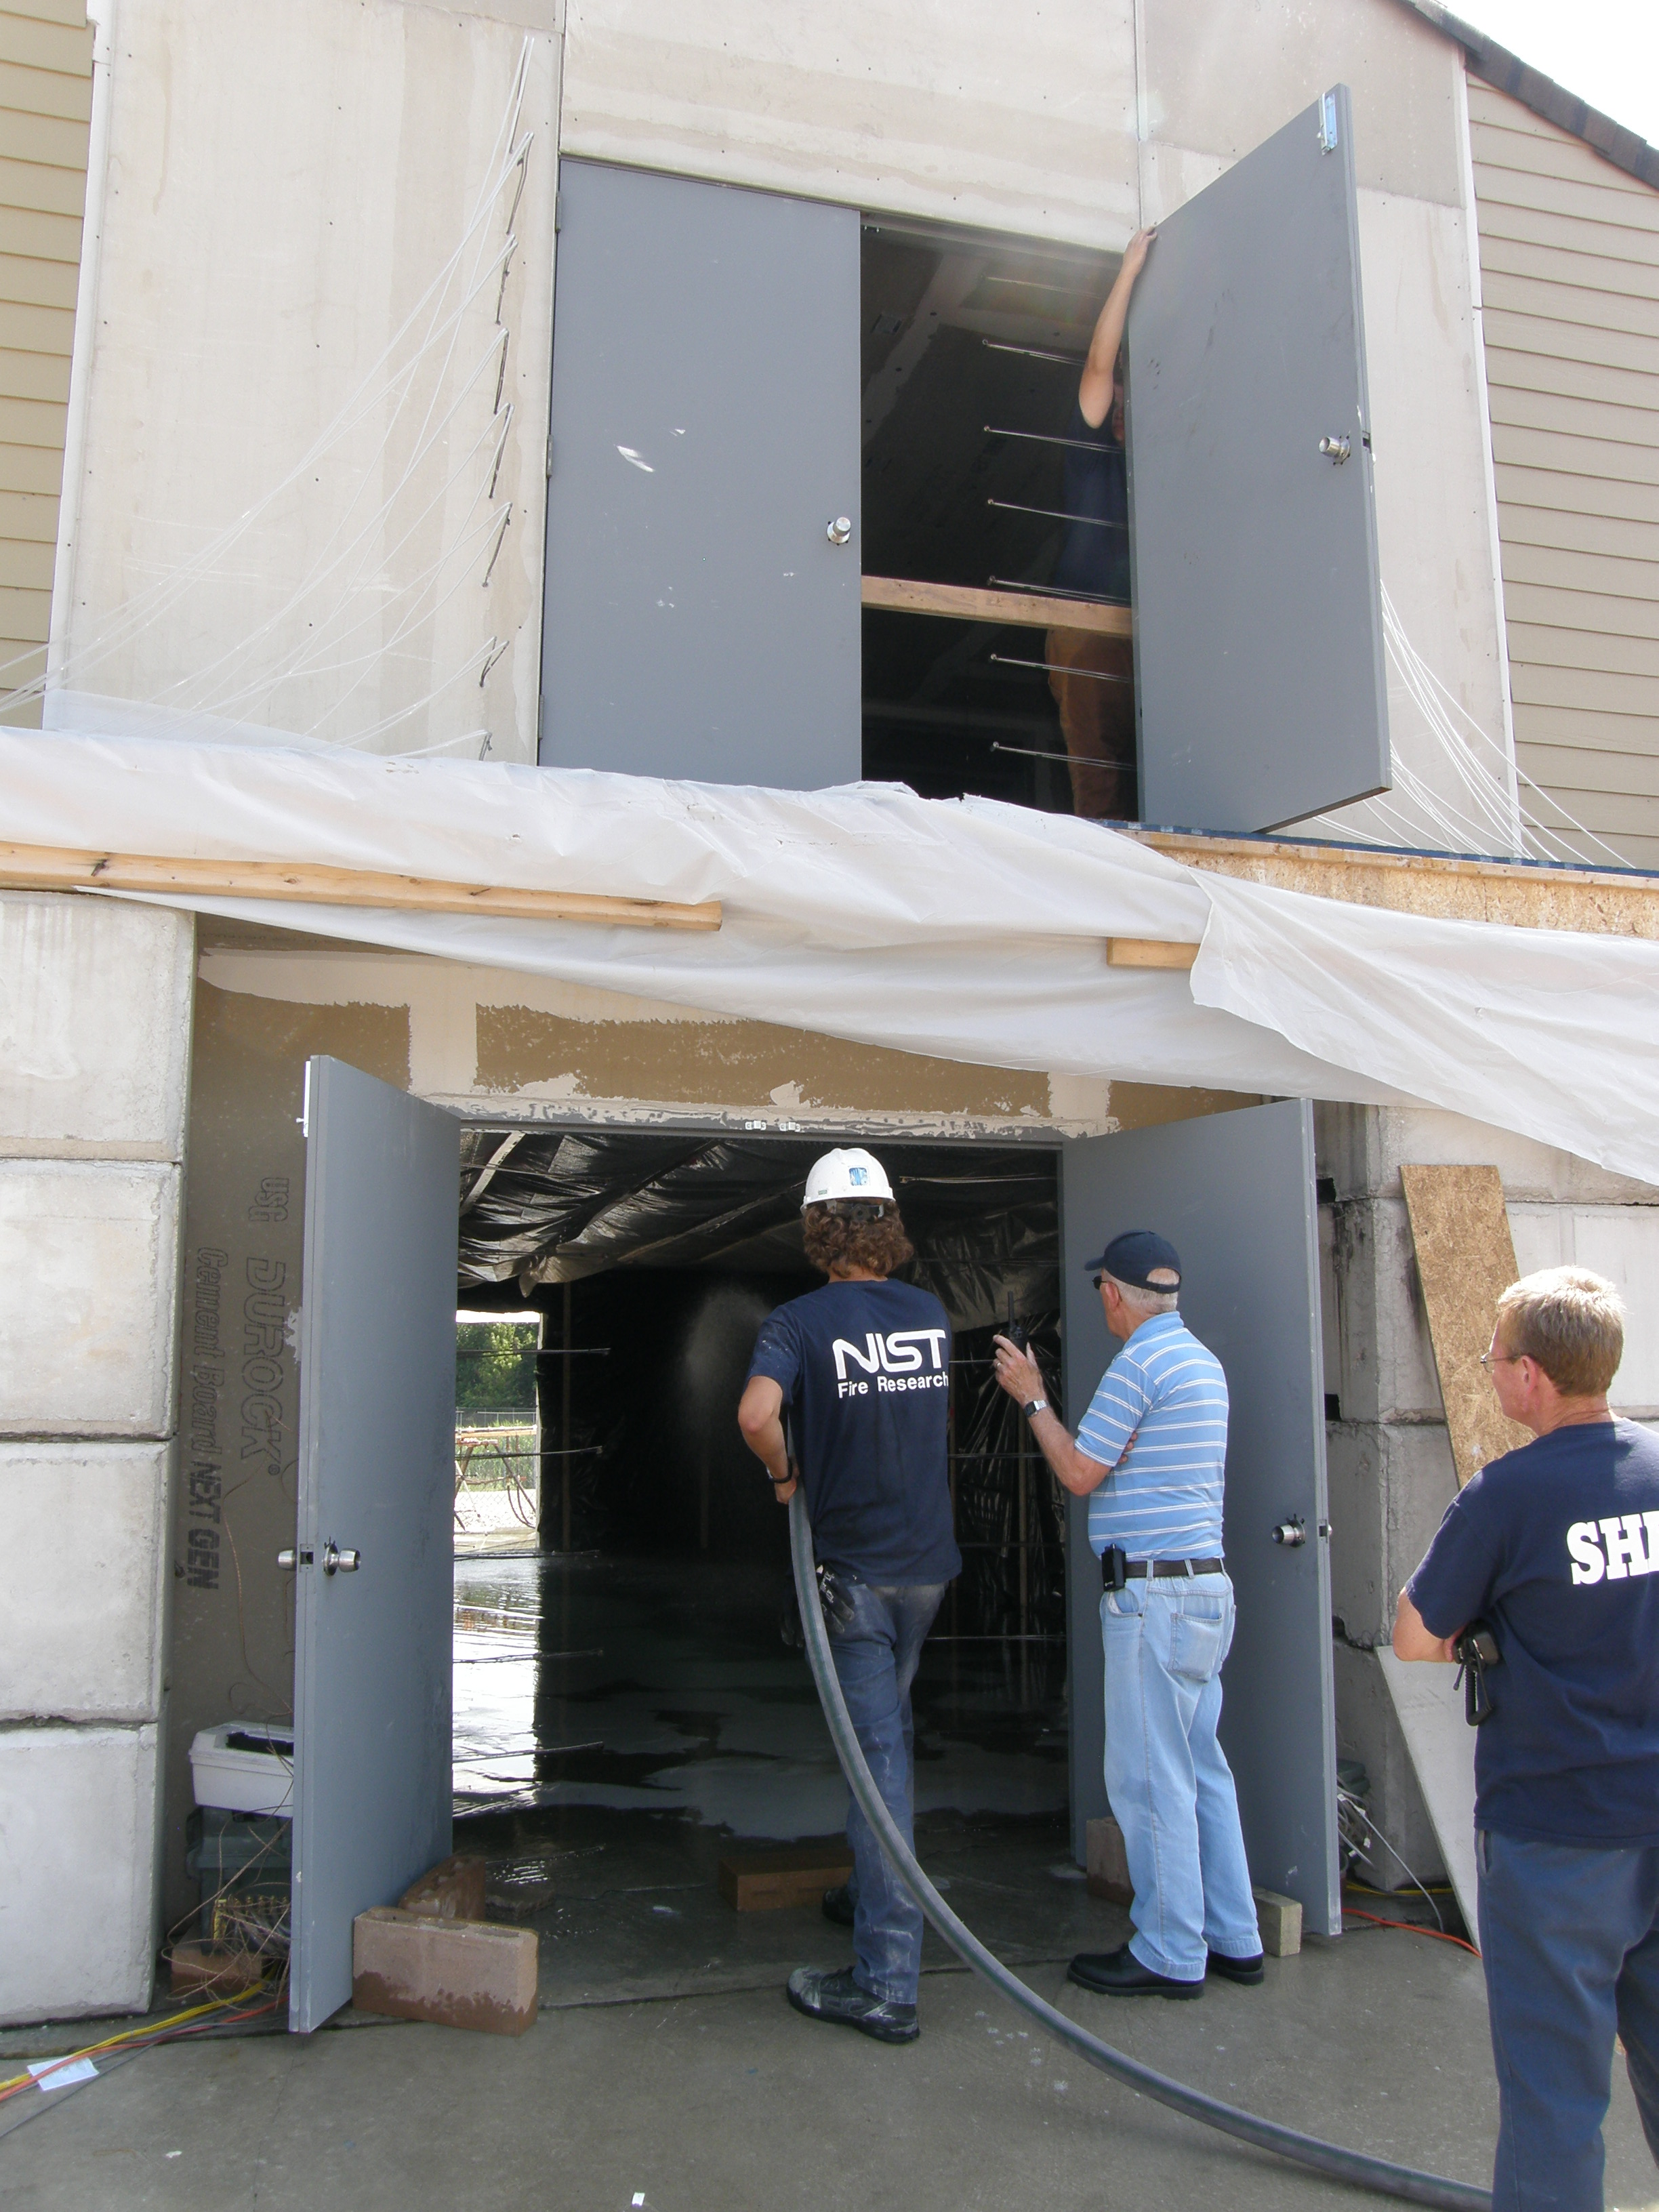
\includegraphics[width=4.25in]{../Figures/Pictures/Test_18}
	\caption[North side of Two Story Structure containing a fully established flow path during Test~6.]{North side of Two Story Structure containing a fully established flow path while water is flowed in a straight stream pattern during Test~6.}
	\label{fig:test_6_pic}
\end{figure}
\FloatBarrier

% ==========================
% = RESULTS AND DISCUSSION =
% ==========================
\chapter{Results and Discussion}
\label{chap:results}
In the following sections, the measurements are presented in graphic and tabular form. In the graphs, an error bar will represent the estimated uncertainty of the measurement. In the tables, the uncertainty will be included in the caption of the table as a percentage enclosed in brackets.

\section{Monitor Experiments}
\label{sec:monitor_results}
Fig.~\ref{fig:Test_2_BDP_A10_Avg_All} contains a plot of the average gas velocity measured by the bi-directional probes in the array at the interior stairwell door (A10) for the straight stream, narrow fog stream, and wide fog stream during Test~2. Similar plots of the average measured velocity through the interior doorway for Tests~1, 3, and 4 are presented in Appendix~\ref{chap:monitor_plots}. Additionally, Table~\ref{table:all_mon_vel_avgs} lists the average velocity measured by the bi-directional probes in A10 when the flow path was fully established for each hose stream and target location combination studied during Tests~1--4.

\begin{figure}[!ht]
	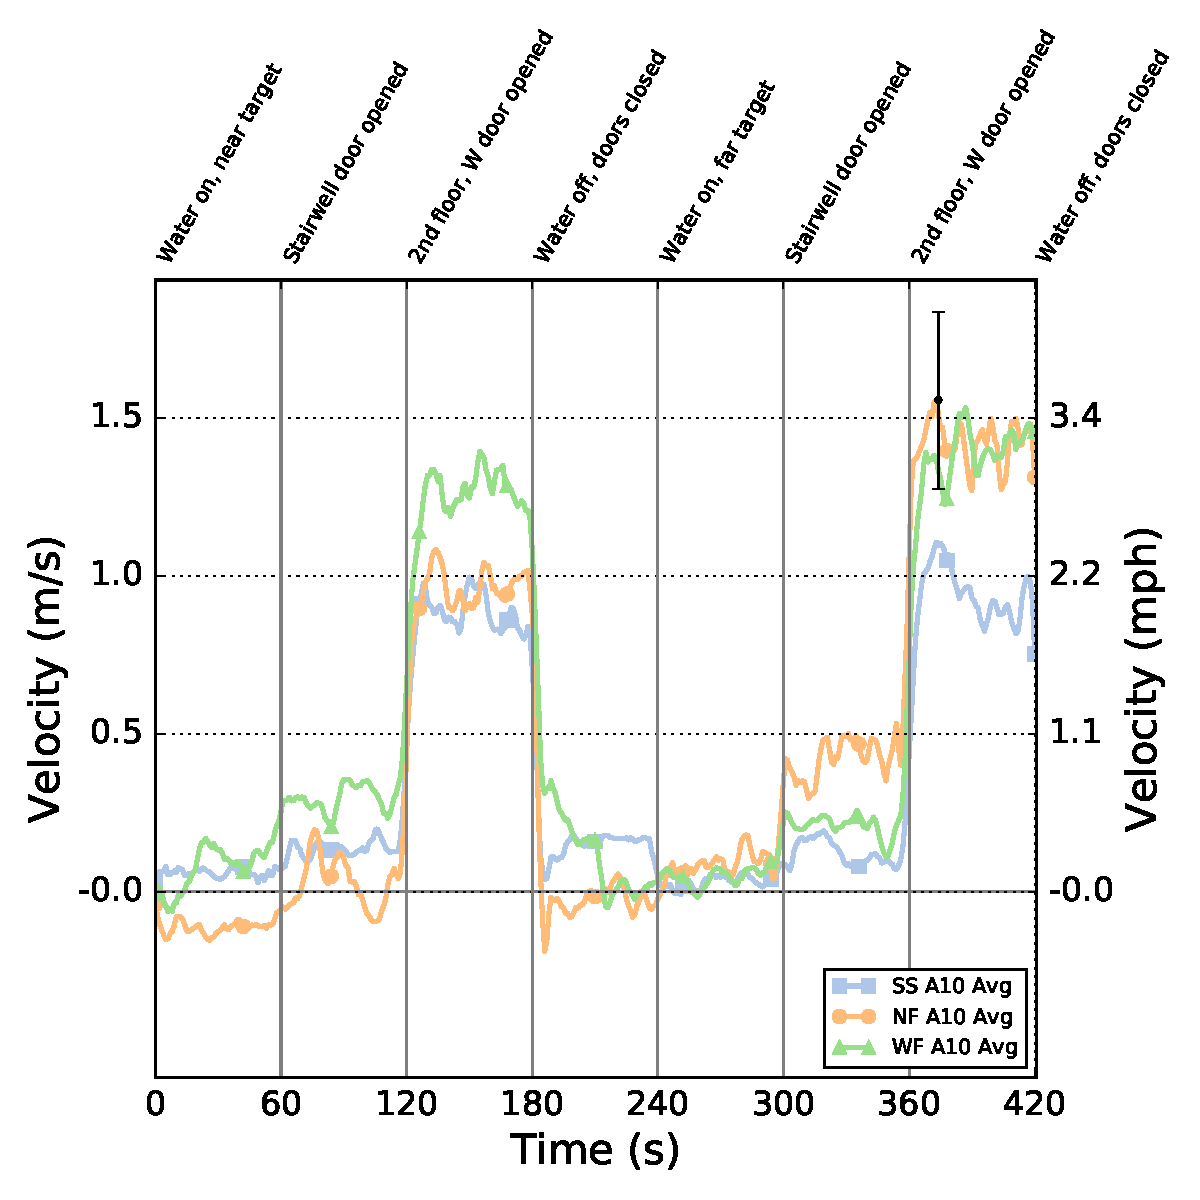
\includegraphics[width=\columnwidth]{../Figures/Plots/Test_16_West_063014_BDP_A10_stream_avgs}
	\caption[Average gas velocity through the interior stairwell door during Test~2 for the three hose stream patterns.]{Average gas velocity measured by the bi-directional probes at the interior stairwell door (A10) during Test~2 for the three hose stream patterns.}
	\label{fig:Test_2_BDP_A10_Avg_All}
\end{figure}

\begin{table}
\footnotesize
\caption{Average gas velocity and airflow rate [$\pm 18$~\%] through interior doorway when flow path was fully established for each monitor experiment}
\begin{tabular}{lccccccccc}
\toprule
 &  &  & \multicolumn{7}{c}{\normalsize ----------------------------------- 120 gpm -----------------------------------} 
\\
 &  &  & \underline{\small Test 1} &  & \multicolumn{2}{c}{\underline{\small Test 2}} &  & \multicolumn{2}{c}{\underline{\small Test 3}}
\\
\textbf{Stream} & \textbf{Value} & \textbf{Units} &
\begin{tabular}{@{}c@{}} \textbf{Room B} \\ \textbf{South} \\ \textbf{Doorway} \end{tabular} &  &
\begin{tabular}{@{}c@{}} \textbf{Near} \\ \textbf{Target} \\ \end{tabular} & \begin{tabular}{@{}c@{}} \textbf{Far} \\ \textbf{Target} \\ \end{tabular} &  &
\begin{tabular}{@{}c@{}} \textbf{Near} \\ \textbf{Target} \\ \end{tabular} & \begin{tabular}{@{}c@{}} \textbf{Far} \\ \textbf{Target} \\ \end{tabular}
\\ 
\midrule
\multirow{5}{*}{\textit{\small Straight}} & \multirow{2}{*}{Velocity}
& 		 m/s 	&	 -0.3 $\pm0.1$		& &	 0.9 $\pm0.2$ 	&	 0.9 $\pm0.2$	& &	 0.7 $\pm0.1$	&	 0.7 $\pm0.1$ \\
&	&	(mph) 	& 	(-0.7 $\pm0.1$) 	& &	(2.0 $\pm0.4$)	&	(2.1 $\pm0.4$)	& &	(1.5 $\pm0.3$)	&	(1.5 $\pm0.3$) 
\\~\\
&	\multirow{2}{*}{ \begin{tabular}{@{}c@{}} Airflow \\ Rate \end{tabular}} 
&	 	m$^3$/s	&	 -0.6 $\pm0.1$   	& &  1.5 $\pm0.3$	&	 1.5 $\pm0.3$  	& &  1.1 $\pm0.2$   & 	 1.1 $\pm0.2$ \\
& 	&	(cfm)	& 	(-1250 $\pm200$)	& & (3100 $\pm550$) &	(3250 $\pm600$) & & (2400 $\pm450$) &	(2400 $\pm450$) 
\\~\\
\multirow{5}{*}{\begin{tabular}{@{}c@{}} \textit{\small Narrow} \\ \textit{\small Fog} \end{tabular}} & \multirow{2}{*}{Velocity}
& 		 m/s   	&    1.1 $\pm0.2$  		& &	 1.0 $\pm0.2$	&	 1.4 $\pm0.3$  	& &   0.8 $\pm0.1$  & 	 0.8 $\pm0.1$ \\
&	&	(mph) 	&	(2.5 $\pm0.5$) 		& &	(2.1 $\pm0.4$)	&	(3.2 $\pm0.6$) 	& &  (1.7 $\pm0.3$) & 	(1.7 $\pm0.3$) 
\\~\\
&	\multirow{2}{*}{ \begin{tabular}{@{}c@{}} Airflow \\ Rate \end{tabular}} 
&		m$^3$/s &	 2.1 $\pm0.4$   	& &  1.6 $\pm0.3$	&	 2.4 $\pm0.4$  	& &  1.3 $\pm0.2$   & 	 1.2 $\pm0.2$ \\
& 	&	(cfm)	&	(4500 $\pm800$)		& & (3350 $\pm600$) &	(5000 $\pm900$) & & (2750 $\pm500$) &	(2650 $\pm450$)
\\~\\
\multirow{5}{*}{\begin{tabular}{@{}c@{}} \textit{\small Wide} \\ \textit{\small Fog} \end{tabular}} & 
\multirow{2}{*}{Velocity}
& 		 m/s   	&	 2.5 $\pm0.4$  		& &  1.3 $\pm0.2$	&	 1.4 $\pm0.2$   & &	 1.2 $\pm0.2$  	& 	 0.8 $\pm0.1$ \\
& 	& 	(mph) 	&	(5.6 $\pm1.0$) 		& & (2.8 $\pm0.5$)	&	(3.1 $\pm0.6$)  & & (2.7 $\pm0.5$) 	& 	(1.7 $\pm0.3$) 
\\~\\
&	\multirow{2}{*}{ \begin{tabular}{@{}c@{}} Airflow \\ Rate \end{tabular}} 
&	 	m$^3$/s	&	 4.6 $\pm0.8$   	& &  2.1 $\pm0.4$	&	 2.3 $\pm0.4$  	& &  2.0 $\pm0.4$   & 	 1.3 $\pm0.2$ \\
& 	&	(cfm)	& 	(9800 $\pm1750$)	& & (4400 $\pm800$) &	(4800 $\pm850$) & & (4200 $\pm750$) &	(2750 $\pm500$)
\\
\midrule
 &  & 	& 	\multicolumn{3}{c}{\normalsize -------- 180 gpm --------} & \multicolumn{4}{c}{} 
\\
 &  & 	&	\multicolumn{3}{c}{\underline{\small Test 4}} & \multicolumn{4}{c}{} 
\\
\textbf{Stream} & \textbf{Value} & \textbf{Units} &
\begin{tabular}{@{}c@{}} \textbf{Near} \\ \textbf{Target} \\ \end{tabular} &
 \multicolumn{2}{c}{\begin{tabular}{@{}c@{}} \textbf{Far} \\ \textbf{Target} \\ \end{tabular}} &
\multicolumn{4}{c}{} 
\\
\midrule
\multirow{5}{*}{\textit{\small Straight}} & \multirow{2}{*}{Velocity}
& 		 m/s   	&	 1.8 $\pm0.3$		&	\multicolumn{2}{c}{ 2.0 $\pm0.4$}		& \multicolumn{4}{c}{} \\
& 	&	(mph) 	&	(3.9 $\pm0.7$) 		&	\multicolumn{2}{c}{(4.4 $\pm0.8$)}		& \multicolumn{4}{c}{} 
\\~\\
&	\multirow{2}{*}{ \begin{tabular}{@{}c@{}} Airflow \\ Rate \end{tabular}} 
&		m$^3$/s &	 2.9 $\pm0.5$  		& 	\multicolumn{2}{c}{ 3.2 $\pm0.6$}		& \multicolumn{4}{c}{} \\
& 	&	(cfm)	&	(6150 $\pm1100$) 	&	\multicolumn{2}{c}{(6900 $\pm1250$)}	& \multicolumn{4}{c}{}
\\~\\
\multirow{5}{*}{\begin{tabular}{@{}c@{}} \textit{\small Smooth} \\ \textit{\small Bore} \end{tabular}} &
\multirow{2}{*}{Velocity}
&		 m/s  	&	 1.8 $\pm0.3$		&	\multicolumn{2}{c}{ 2.1 $\pm0.4$}		& \multicolumn{4}{c}{} \\
&	&	(mph)	&	(4.0 $\pm0.7$)		&	\multicolumn{2}{c}{(4.8 $\pm0.9$)}		& \multicolumn{4}{c}{}
\\~\\
&	\multirow{2}{*}{ \begin{tabular}{@{}c@{}} Airflow \\ Rate \end{tabular}} 
&		m$^3$/s &	 3.0 $\pm0.5$		& 	\multicolumn{2}{c}{ 3.5 $\pm0.6$} 		& \multicolumn{4}{c}{} \\
& 	&	(cfm)	&	(6250 $\pm1150$) 	&	\multicolumn{2}{c}{(7450 $\pm1350$)} 	& \multicolumn{4}{c}{}
\\
\bottomrule
\end{tabular}
\label{table:all_mon_vel_avgs}
\end{table}

Looking at the table and figures, a number of trends can be observed. For example, there was air movement---an average gas velocity greater than 0.5~m/s (1.1~mph)---through the interior doorway while the flow path was fully established for every hose stream and target location combination except the straight stream in Test~1. Looking at Table~\ref{table:all_mon_vel_avgs}, the narrow fog and wide fog streams caused higher velocities through the interior doorway when the flow path was fully established compared to the straight stream. This trend can also be seen graphically in Fig.~\ref{fig:Test_2_BDP_A10_Avg_All} and Figs.~\ref{fig:Test_1_BDP_A6_Avg_All}~and~\ref{fig:Test_3_BDP_A10_Avg_All} in Appendix~\ref{chap:monitor_plots}. Furthermore, the wide fog stream generally produced equal or higher air velocities compared to the narrow fog stream. Finally, the Test~4 results listed in Table~\ref{table:all_mon_vel_avgs} and plotted in Fig.~\ref{fig:Test_4_BDP_A10_Avg_All} suggest that the straight stream from a combination nozzle and the solid stream from a smooth bore nozzle equipped with a 1~in tip produced approximately the same amount of air movement through the interior doorway.
\FloatBarrier

\section{Handline Experiments}
\label{sec:handline_results}
Fig.~\ref{fig:Test_6_BDP_A10_Avg_All} contains a plot of the average gas velocity measured by the bi-directional probes in the array at the interior stairwell door (A10) for the straight stream, narrow fog stream, and wide fog stream being applied in a fixed position, a sweeping pattern (back and forth, left-to-right), a clockwise rotation, and a counterclockwise rotation during Test~6. Similar plots of the average measured velocity through the interior doorway for Tests~5 and 7 are presented in Appendix~\ref{chap:handline_plots}. Additionally, Tables~\ref{table:east_hand_A6_avgs}~and~\ref{table:west_hand_A10_avgs} list the average velocity measured by the bi-directional probes in A10 when the flow path was fully established for each hose stream and nozzle movement pattern combination studied during Test~5 and Tests~6--7, respectively.

\begin{figure}[!ht]
	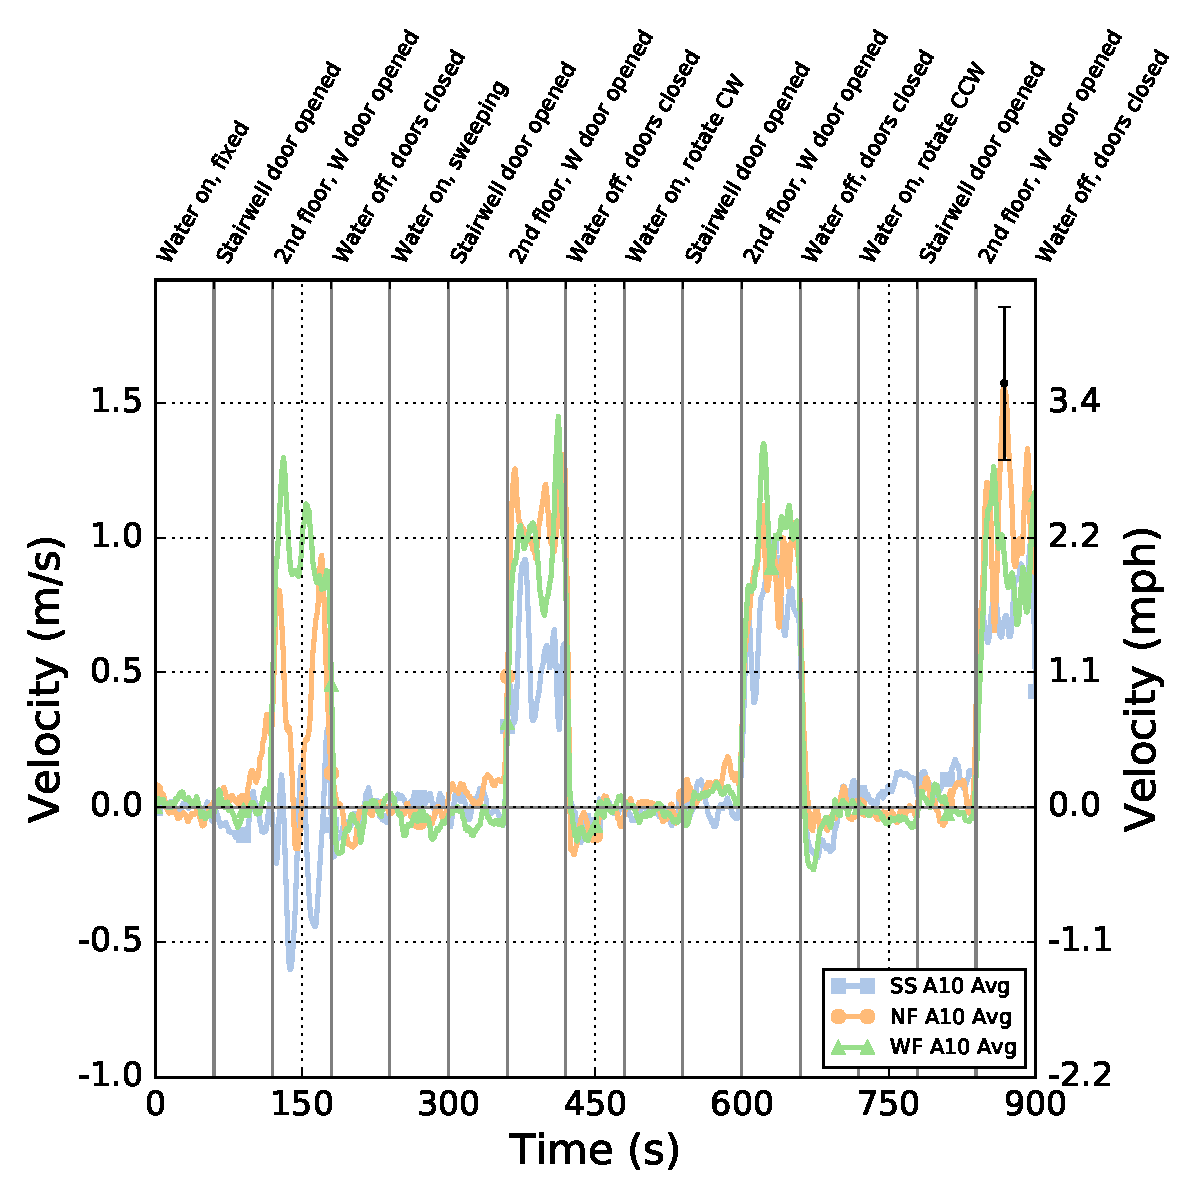
\includegraphics[width=\columnwidth]{../Figures/Plots/Test_18_West_063014_BDP_A10_stream_avgs}
	\caption[Average gas velocity through the interior stairwell door during Test~6 for the three hose stream patterns.]{Average gas velocity measured by the bi-directional probes at the interior stairwell door (A10) during Test~6 for the three hose stream patterns.}
	\label{fig:Test_6_BDP_A10_Avg_All}
\end{figure}
\FloatBarrier

\begin{table}[!ht]
\caption{Average gas velocity and airflow rate [$\pm 18$~\%] through interior doorway when flow path was fully established for Test~5}
\begin{tabular}{lccccc}
\toprule
 &	&	&	\multicolumn{3}{c}{\underline{Room A}}
\\
\textbf{Stream} & \textbf{Value} & \textbf{Units} &
\textbf{Fixed} & \textbf{Clockwise} & \begin{tabular}{@{}c@{}} \textbf{Counter} \\ \textbf{Clockwise} \\ \end{tabular}
\\ \midrule
\multirow{5}{*}{\textit{Straight}} & \multirow{2}{*}{\small Velocity}
& 		 \small{m/s}   	&   0.2 $\pm0.03$	&   0.7 $\pm0.1$	&	 0.8 $\pm0.2$  \\ 
&	&	 \small{(mph)} 	&  (0.4 $\pm0.1$)	&  (1.5 $\pm0.3$)	&	(1.9 $\pm0.3$)
\\~\\
&	\multirow{2}{*}{ \begin{tabular}{@{}c@{}} \small{Airflow} \\ \small{Rate} \end{tabular}} 
&	 	\small{m$^3$/s}	&	 0.3 $\pm0.1$	&  1.2 $\pm0.2$		&	 1.6 $\pm0.3$  	\\
& 	&	\small{(cfm)}	& 	(628 $\pm113$)	& (2584 $\pm465$) 	&	(3291 $\pm592$)
\\~\\
\multirow{5}{*}{\begin{tabular}{@{}c@{}} \textit{Narrow} \\ \textit{Fog} \end{tabular}} & \multirow{2}{*}{\small Velocity}
& 		\small{m/s}   	&	 1.7 $\pm0.3$   	&	 1.8 $\pm0.3$  	&   1.6 $\pm0.3$   \\
&	&	\small{(mph)} 	&	(3.9 $\pm0.7$) 		&	(4.0 $\pm0.7$) 	&  (3.5 $\pm0.6$)
\\~\\
&	\multirow{2}{*}{ \begin{tabular}{@{}c@{}} \small{Airflow} \\ \small{Rate} \end{tabular}} 
&	 	\small{m$^3$/s}	&	 3.2 $\pm0.6$   	&	 3.3 $\pm0.6$		&	 2.9 $\pm0.5$  	\\
& 	&	\small{(cfm)}	& 	(6786 $\pm1222$)	&	(6977 $\pm1256$) 	&	(6228 $\pm1121$)
\\~\\
\multirow{5}{*}{\begin{tabular}{@{}c@{}} \textit{Wide} \\ \textit{Fog} \end{tabular}} & \multirow{2}{*}{\small Velocity} 
&		\small{m/s} 	&	 1.8 $\pm0.3$   	&   2.1 $\pm0.4$  	&   2.2 $\pm0.4$  \\ 
& 	& 	\small{(mph)}	&	(4.1 $\pm0.7$)  	&  (4.8 $\pm0.9$) 	&  (4.9 $\pm0.9$)  
\\ ~\\
&	\multirow{2}{*}{ \begin{tabular}{@{}c@{}} \small{Airflow} \\ \small{Rate} \end{tabular}} 
&	 	\small{m$^3$/s}	&	 3.4 $\pm0.6$   	&  4.0 $\pm0.7$		&	 4.1 $\pm0.7$  	\\
& 	&	\small{(cfm)}	& 	(7283 $\pm1311$)	& (8463 $\pm1523$) 	&	(8669 $\pm1561$) \\
\midrule
&	&	&	\multicolumn{3}{c}{\underline{Room B Ceiling}}
\\
\textbf{Stream} & \textbf{Value} & \textbf{Units} &
\textbf{Fixed} & \textbf{Clockwise} & \begin{tabular}{@{}c@{}} \textbf{Counter} \\ \textbf{Clockwise} \\ \end{tabular}
\\ \midrule
\multirow{5}{*}{\textit{Straight}} & \multirow{2}{*}{\small Velocity}
& 		 \small{m/s}   	&   -0.1 $\pm0.02$    	&   0.6 $\pm0.1$   	&	 0.5 $\pm0.1$  \\ 
&	&	 \small{(mph)} 	&  (-0.2 $\pm0.04$)  	&  (1.4 $\pm0.3$) 	&	(1.2 $\pm0.2$)
\\~\\
&	\multirow{2}{*}{ \begin{tabular}{@{}c@{}} \small{Airflow} \\ \small{Rate} \end{tabular}} 
&	 	\small{m$^3$/s}	&	 -0.2 $\pm0.03$   	&  1.2 $\pm0.2$		&	 1.0 $\pm0.2$  	\\
& 	&	\small{(cfm)}	& 	(-381 $\pm69$)		& (2469 $\pm445$) 	&	(2155 $\pm388$)
\\~\\
\multirow{5}{*}{\begin{tabular}{@{}c@{}} \textit{Narrow} \\ \textit{Fog} \end{tabular}} & \multirow{2}{*}{\small Velocity}
& 		\small{m/s}   	&   0.9 $\pm0.2$   		&   1.5 $\pm0.3$  	&   1.6 $\pm0.3$   \\
&	&	\small{(mph)} 	&  (2.1 $\pm0.4$)  		&  (3.4 $\pm0.6$) 	&  (3.7 $\pm0.7$)
\\~\\
&	\multirow{2}{*}{ \begin{tabular}{@{}c@{}} \small{Airflow} \\ \small{Rate} \end{tabular}} 
&	 	\small{m$^3$/s}	&	 1.8 $\pm0.3$   	&  2.9 $\pm0.5$		&	 3.1 $\pm0.6$  	\\
& 	&	\small{(cfm)}	& 	(3739 $\pm673$)		& (6046 $\pm1088$) 	&	(6479 $\pm1166$)
\\~\\
\multirow{5}{*}{\begin{tabular}{@{}c@{}} \textit{Wide} \\ \textit{Fog} \end{tabular}} & \multirow{2}{*}{\small Velocity} 
&		\small{m/s} 	&   2.1 $\pm0.4$   		&   2.3 $\pm0.4$  	&   2.6 $\pm0.5$  \\ 
& 	& 	\small{(mph)}	&  (4.7 $\pm0.8$)  		&  (5.2 $\pm0.9$) 	&  (5.8 $\pm1.1$)  
\\ ~\\
&	\multirow{2}{*}{ \begin{tabular}{@{}c@{}} \small{Airflow} \\ \small{Rate} \end{tabular}} 
&	 	\small{m$^3$/s}	&	 3.9 $\pm0.7$   	&  4.3 $\pm0.8$		&	 4.8 $\pm0.9$  	\\
& 	&	\small{(cfm)}	& 	(8271 $\pm1489$)	& (9165 $\pm1650$) 	&	(10273 $\pm1849$) \\
\bottomrule
\end{tabular}
\label{table:east_hand_A6_avgs}
\end{table}

\begin{table}[!ht]
\caption{Average gas velocity and airflow rate [$\pm18$~\%] through interior doorway when flow path was fully established for Tests~6 and 7}
\begin{tabular}{lcccccc}
\toprule
&	&	&	\multicolumn{4}{c}{\underline{Test 6}}
\\
\textbf{Stream} & \textbf{Value} & \textbf{Units} &
\textbf{Fixed} & \textbf{Sweeping} & \textbf{Clockwise} & 
\begin{tabular}{@{}c@{}} \textbf{Counter} \\ \textbf{Clockwise} \\ \end{tabular}
\\ \midrule
\multirow{5}{*}{\textit{Straight}} & \multirow{2}{*}{\small Velocity} 
& 		\small{m/s}		&   -0.2 $\pm0.03$   &   0.5 $\pm0.1$  &   0.7 $\pm0.1$   &  0.7 $\pm0.1$  \\ 
&	&	\small{(mph)}	&  (-0.4 $\pm0.1$)  &  (1.2 $\pm0.2$) &  (1.6 $\pm0.3$)  & (1.7 $\pm0.3$)
\\~\\
&	\multirow{2}{*}{ \begin{tabular}{@{}c@{}} \small{Airflow} \\ \small{Rate} \end{tabular}} 
&	 	\small{m$^3$/s}	&	 -0.3 $\pm0.1$		&	 0.9 $\pm0.2$		&	 1.2 $\pm0.2$		&	 1.2 $\pm0.2$  	\\
& 	&	\small{(cfm)}	& 	(-670 $\pm121$)		&	(1864 $\pm336$)		&	(2549 $\pm459$)		& 	(2602 $\pm468$)
\\~\\
\multirow{5}{*}{\begin{tabular}{@{}c@{}} \textit{Narrow} \\ \textit{Fog} \end{tabular}} & \multirow{2}{*}{\small Velocity}
&		\small{m/s}   	&	 0.4 $\pm0.1$   	&	 1.1 $\pm0.2$		&	 0.9 $\pm0.2$		&	 1.1 $\pm0.2$  \\ 
&	&	\small{(mph)} 	&	(0.9 $\pm0.2$)  	&	(2.4 $\pm0.4$)		&	(1.9 $\pm0.3$)		& 	(2.4 $\pm0.4$)
\\~\\
&	\multirow{2}{*}{ \begin{tabular}{@{}c@{}} \small{Airflow} \\ \small{Rate} \end{tabular}} 
&	 	\small{m$^3$/s}	&	 0.7 $\pm0.1$   	&	 1.7 $\pm0.3$		&	 1.4 $\pm0.3$  		&	 1.8 $\pm0.3$  	\\
& 	&	\small{(cfm)}	& 	(1471 $\pm265$)		&	(3688 $\pm664$) 	&	(3034 $\pm546$)		& 	(3786 $\pm682$)
\\~\\
\multirow{5}{*}{\begin{tabular}{@{}c@{}} \textit{Wide} \\ \textit{Fog} \end{tabular}} & \multirow{2}{*}{\small Velocity}
&		\small{m/s}   	&    1.0 $\pm0.2$   	&	 1.0 $\pm0.2$  		&	 1.0 $\pm0.2$   	&  	 0.9 $\pm0.2$  \\  
&	&	\small{(mph)} 	&	(2.2 $\pm0.4$)  	&	(2.1 $\pm0.4$) 		&  	(2.2 $\pm0.4$)  	& 	(2.0 $\pm0.4$) 
\\~\\
&	\multirow{2}{*}{ \begin{tabular}{@{}c@{}} \small{Airflow} \\ \small{Rate} \end{tabular}} 
&	 	\small{m$^3$/s}	&	 1.6 $\pm0.3$   	&	 1.6 $\pm0.3$		&	 1.6 $\pm0.3$  		&	 1.4 $\pm0.3$  	\\
& 	&	\small{(cfm)}	& 	(3369 $\pm606$)		&	(3362 $\pm605$) 	&	(3453 $\pm622$)		& 	(3051 $\pm549$)
\\ \midrule
& 	& 	&	\multicolumn{4}{c}{\underline{Test 7}}
\\
\textbf{Stream} & \textbf{Value} & \textbf{Units} &
\textbf{Fixed} & \textbf{Sweeping} & \textbf{Clockwise} & 
\begin{tabular}{@{}c@{}} \textbf{Counter} \\ \textbf{Clockwise} \\ \end{tabular}
\\ \midrule
\multirow{5}{*}{\textit{Straight}} & \multirow{2}{*}{\small Velocity}
&		\small{m/s}   	&	 0.0 $\pm0.01$		&	 0.5 $\pm0.1$  		&	 0.7 $\pm0.1$   	&	 0.7 $\pm0.1$  \\ 
&	&	\small{(mph)} 	&	(-0.1 $\pm0.02$)	&	(1.2 $\pm0.2$)		&	(1.6 $\pm0.3$)  	&	(1.5 $\pm0.3$)
\\~\\
&	\multirow{2}{*}{ \begin{tabular}{@{}c@{}} \small{Airflow} \\ \small{Rate} \end{tabular}} 
&	 	\small{m$^3$/s}	&	 -0.1 $\pm0.01$   	&	 0.9 $\pm0.2$		&	 1.2 $\pm0.2$		&	 1.1 $\pm0.2$  	\\
& 	&	\small{(cfm)}	& 	(-152 $\pm27$)		&	(1804 $\pm325$) 	&	(2473 $\pm445$)		& 	(2358 $\pm425$)
\\~\\
\multirow{5}{*}{\begin{tabular}{@{}c@{}} \textit{Narrow} \\ \textit{Fog} \end{tabular}} & \multirow{2}{*}{\small Velocity} 
&		\small{m/s}   	&	 1.3 $\pm0.2$   	&	 1.2 $\pm0.2$  		&	 1.2 $\pm0.2$   	&	 1.3 $\pm0.2$  \\ 
&	&	\small{(mph)} 	&	(2.9 $\pm0.5$)  	&	(2.8 $\pm0.5$) 		&	(2.7 $\pm0.5$)  	&	(2.9 $\pm0.5$)
\\~\\
&	\multirow{2}{*}{ \begin{tabular}{@{}c@{}} \small{Airflow} \\ \small{Rate} \end{tabular}} 
&	 	\small{m$^3$/s}	&	 2.1 $\pm0.4$   	&  	 2.0 $\pm0.4$		&	 2.0 $\pm0.4$  		& 	 2.1 $\pm0.4$ 	\\
& 	&	\small{(cfm)}	& 	(4494 $\pm809$)		& 	(4326 $\pm779$) 	&	(4214 $\pm759$)		& 	(4477 $\pm806$)
\\~\\
\multirow{5}{*}{\begin{tabular}{@{}c@{}} \textit{Wide} \\ \textit{Fog} \end{tabular}} & \multirow{2}{*}{\small Velocity} 
&		\small{m/s}   	&	 1.0 $\pm0.2$   	&	 0.7 $\pm0.1$  		&	 0.9 $\pm0.2$   	&	 1.0 $\pm0.2$  \\ 
&	&	\small{(mph)} 	&	(2.2 $\pm0.4$)  	&	(1.6 $\pm0.3$) 		&	(2.1 $\pm0.4$)  	& 	(2.2 $\pm0.4$) 
\\~\\ 
&	\multirow{2}{*}{ \begin{tabular}{@{}c@{}} \small{Airflow} \\ \small{Rate} \end{tabular}} 
&	 	\small{m$^3$/s}	&	 1.7 $\pm0.3$   	&	 1.2 $\pm0.2$		&	 1.6 $\pm0.3$  		& 	 1.6 $\pm0.3$	\\
& 	&	\small{(cfm)}	& 	(3509 $\pm632$)		&	(2503 $\pm451$) 	&	(3299 $\pm594$)		& 	(3428 $\pm617$)
\\ \bottomrule
\end{tabular}
\label{table:west_hand_A10_avgs}
\end{table}
\FloatBarrier

With the exception of the narrow fog stream in the fixed position during Test~6, every hose stream and nozzle movement pattern combination using a narrow fog or wide fog stream during the handline experiments produced air movement---an average gas velocity greater than 0.5~m/s (1.1~mph)---through the interior doorway while the flow path was fully established. For the straight stream, however, air movement through the interior doorway only occurred when the stream was applied in a pattern that involved moving the handline. Similar to the monitor experiments, the average air velocity through the interior doorway was always greater in magnitude for the nozzle movement patterns using the narrow and wide fog streams than the same patterns using the straight stream. Another important result seen in Tables~\ref{table:east_hand_A6_avgs} and \ref{table:west_hand_A10_avgs} is that there are no statistically significant differences in the amount of air flow through the interior doorway when rotating the hoseline in the clockwise direction compared to rotating it in the counterclockwise direction for any of three hose streams tested. The similarities in air flow produced by the clockwise and counterclockwise nozzle movement patterns can also be seen graphically in Fig.~\ref{fig:Test_6_BDP_A10_Avg_All} and Figs.~\ref{fig:Test_5_BDP_A6_Avg_All} and \ref{fig:Test_7_BDP_A10_Avg_All} in Appendix~\ref{chap:handline_plots}. 


% ===========
% = Summary =
% ===========
\chapter{Summary}
\label{chap:summary}

A total of seven experimental series were conducted to study the impact of different hose stream and nozzle movement pattern combinations on air movement within residential scale structures. 

Three experimental series studied the differences between a straight stream, narrow fog stream, and wide fog stream emitted from a combination nozzle attached to a monitor aimed at specific locations in a structure for different ventilation configurations. For each of the three series, the average air velocity through the interior doorway while the flow path was fully established was greatest for the wide fog stream no matter the location and ventilation pattern within the structure. The magnitude of the average air velocity through the interior doorway while the flow path was fully established for the narrow fog stream was always equal to or greater than the magnitude of the average air velocity for the straight stream. 

Additionally, a fourth experimental series using a monitor was conducted in which a straight stream from a combination nozzle was compared to a solid stream from a smooth bore nozzle with a 1~in tip aimed at a specified location for 60 seconds with a fully established flow path. The streams were compared for six different 60 seconds periods during which the flow path was fully established: three times each for the monitor aimed at two locations. The results from the four monitor test series suggest a wide fog stream impacts air movement within a structure the most out of any of the tested streams, followed by the narrow fog stream, and then the straight stream and solid stream from a smooth bore nozzle, which both caused approximately the same amount of air movement through the structure.

In addition to the monitor test series, three different experimental series were conducted using a handline to study the impact of different stream and nozzle movement pattern combinations on air movement within a structure. Similar to the monitor experiments, the average air velocity through the interior doorway of a structure with a fully established flow path was greater for the wide fog and narrow fog streams than the straight stream. It was discovered that a straight stream increased air movement through the interior doorway when it was applied in a moving pattern. With regard to Royer's theory, throughout all handline test series, there were no statistically significant differences in the average air velocity measured through the interior doorway between the clockwise and counterclockwise nozzle movement patterns. However, these experiments only addressed cold flow.

For this limited series of water flow experiments, the data demonstrate that for these flows and configurations, hose streams can affect air movement within a structure. The type of hose stream used and manner in which it is applied dictates the extent to which a stream impacts the ventilation of a structure. These experiments have shown there is a potential for hose streams to affect air flows within a structure during fire scenarios. To better quantify the impact of air flows from hose streams on the fire environment, additional experiments need to be conducted with structure fires in a controlled environment.

% ====================
% = ACKNOWLEDGEMENTS =
% ====================
\chapter{Acknowledgments}
\label{chap:acknowledgments}

The authors would like to thank Roy McLane (currently with Thermal Fabrication), Kristopher Overholt (currently with Continuum Analytics), Keith Stakes (currently with UL FSRI), Nicholas Dow (SURF student), and Jay MCElroy (retired) from NIST for their contributions in preparing and conducting these experiments. These experiments could not have been conducted without them. 

The Delaware County Emergency Services Training Center provided the location and logistical support for these experiments.  The Delaware county team was under the direction of Kerby Kerber.  For construction and test support the team included: Joe Bingham, Dave Wright, Dave Nercesian (small engine repair), Mike Gura, Scott Wiercinski, Bill Fields (Fields Fire Protection).  We also thank the dedicated team of fire instructors and firefighters that supported these experiments; Brian Righter (Rudy), John McGowan, Matthew Poissant, John Frey, Brian Embert, Raymond Keller III, Mike Bramble, Edward McBride, Mark Morrissey, Bill Norris, and Matt LeTourneau.

Thank you for assisting NIST in generating data that will assist the fire service in making tactical choices.



\bibliography{../../../../../Bibliography/FDS_general}

\appendix
\chapter{Monitor Test Plots}
\label{chap:monitor_plots}

\begin{figure}[!ht]
	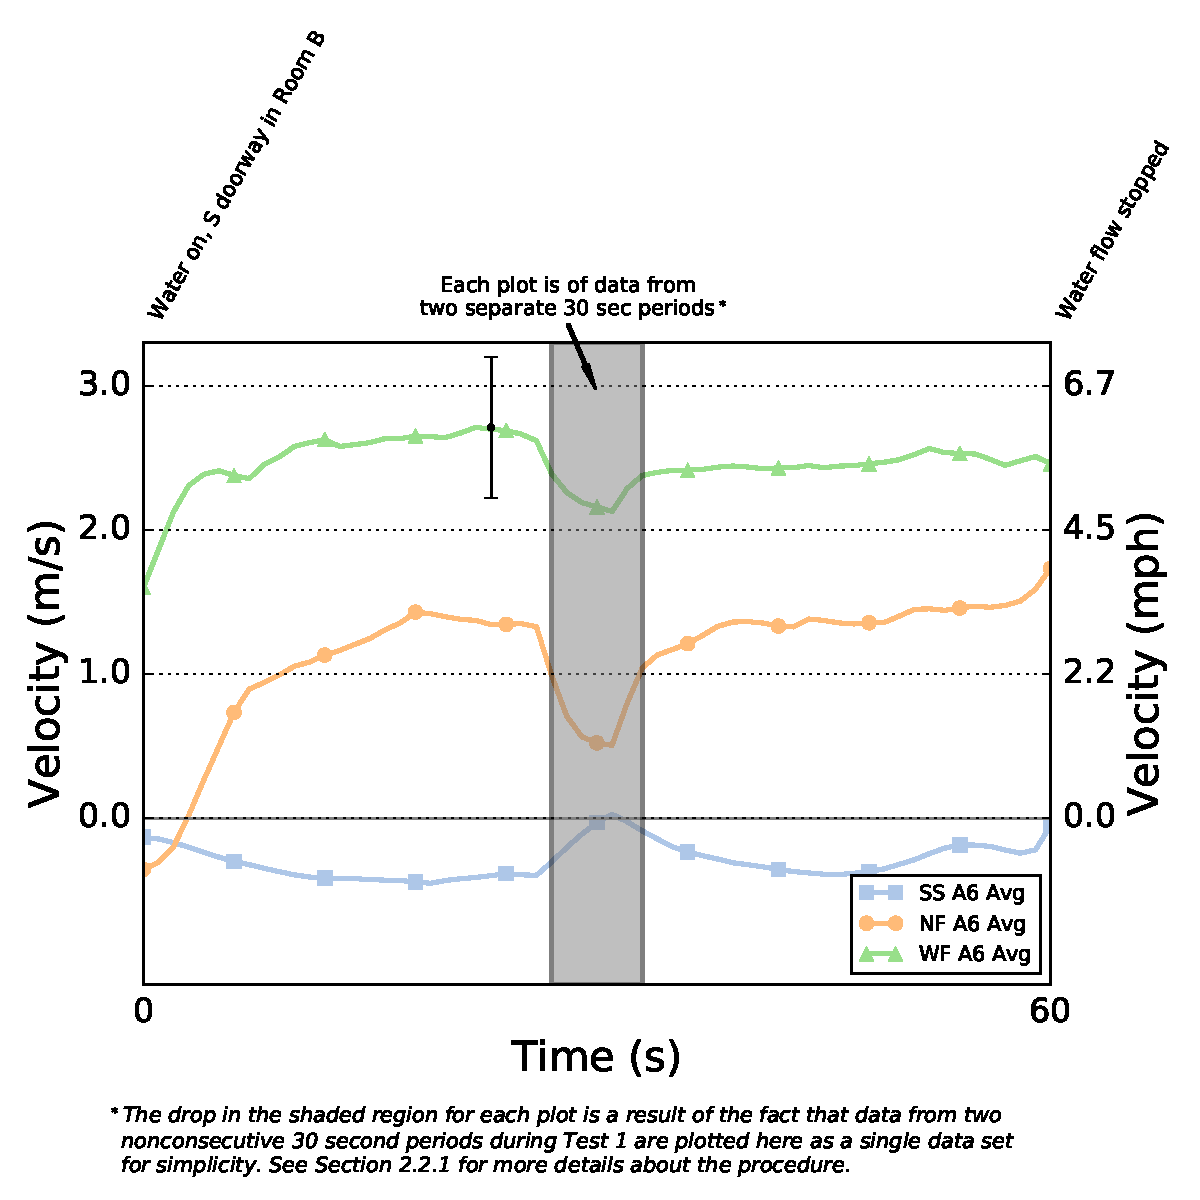
\includegraphics[width=\columnwidth]{../Figures/Plots/HOSE_IXXAXX_BDP_A6_stream_avgs}
	\caption[Average gas velocity through the interior doorway during Test~1 for the three hose stream patterns.]{Average gas velocity measured by the bi-directional probes at the interior doorway (A6) during Test~1 for the three hose stream patterns.}
	\label{fig:Test_1_BDP_A6_Avg_All}
\end{figure}
\FloatBarrier
% Streams were flowed during two 30 second, nonconsecutive periods, but plotted back-to-back for simplicity. See Section 2.2.1 for more details about the procedure

\begin{figure}[!ht]
	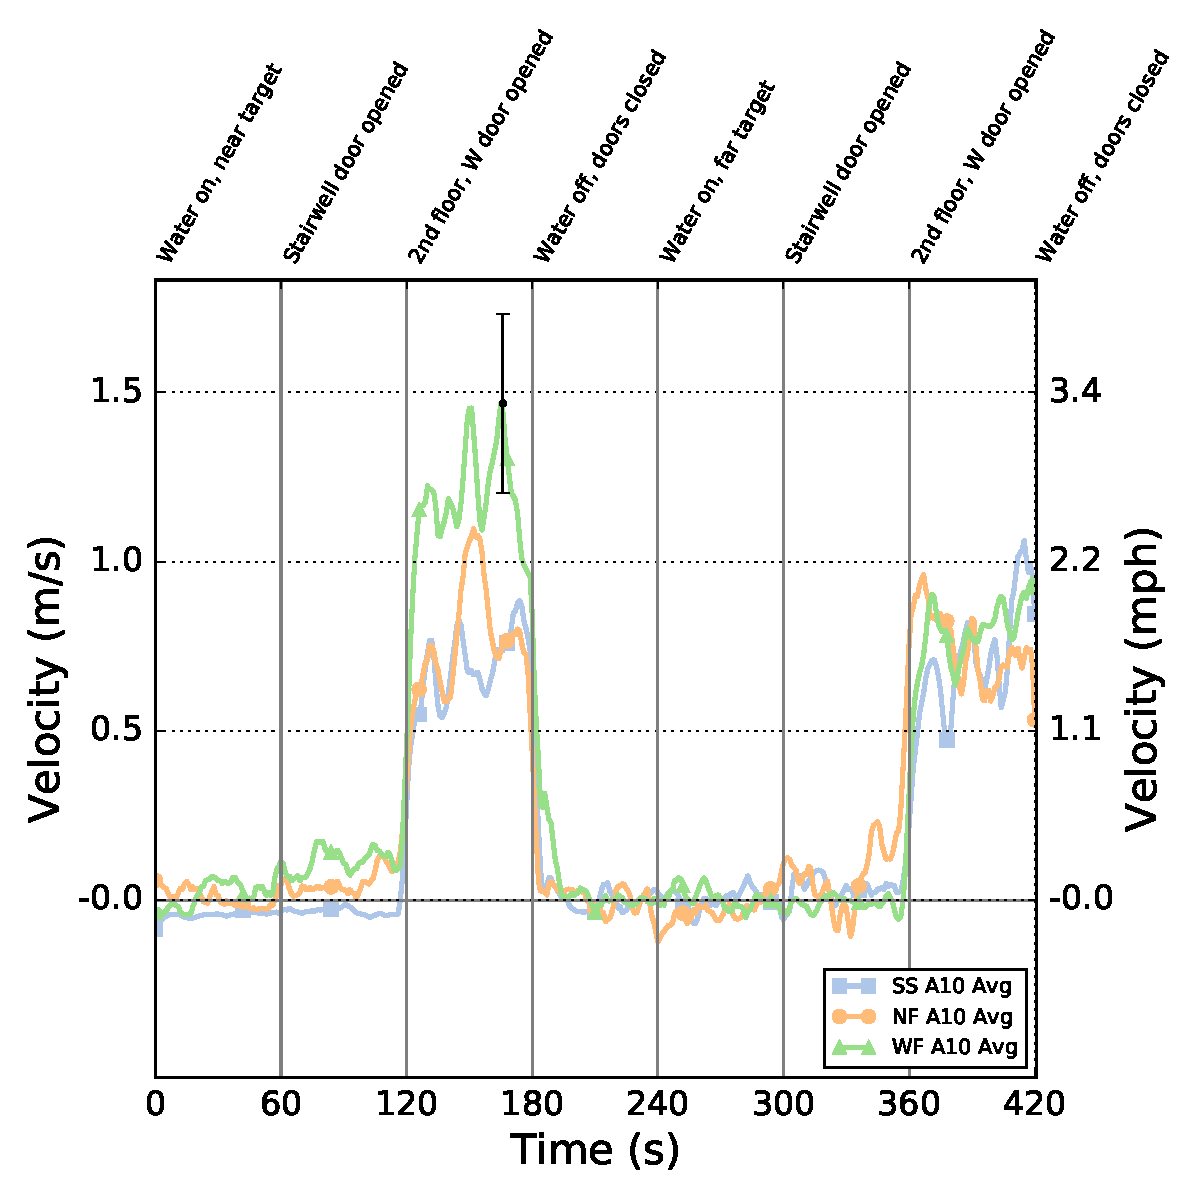
\includegraphics[width=\columnwidth]{../Figures/Plots/Test_17_West_063014_BDP_A10_stream_avgs}
	\caption[Average gas velocity through the interior stairwell door during Test~3 for the three hose stream patterns.]{Average gas velocity measured by the bi-directional probes at the interior stairwell door (A10) during Test~3 for the three hose stream patterns.}
	\label{fig:Test_3_BDP_A10_Avg_All}
	\end{figure}
\FloatBarrier

\begin{figure}[!ht]
	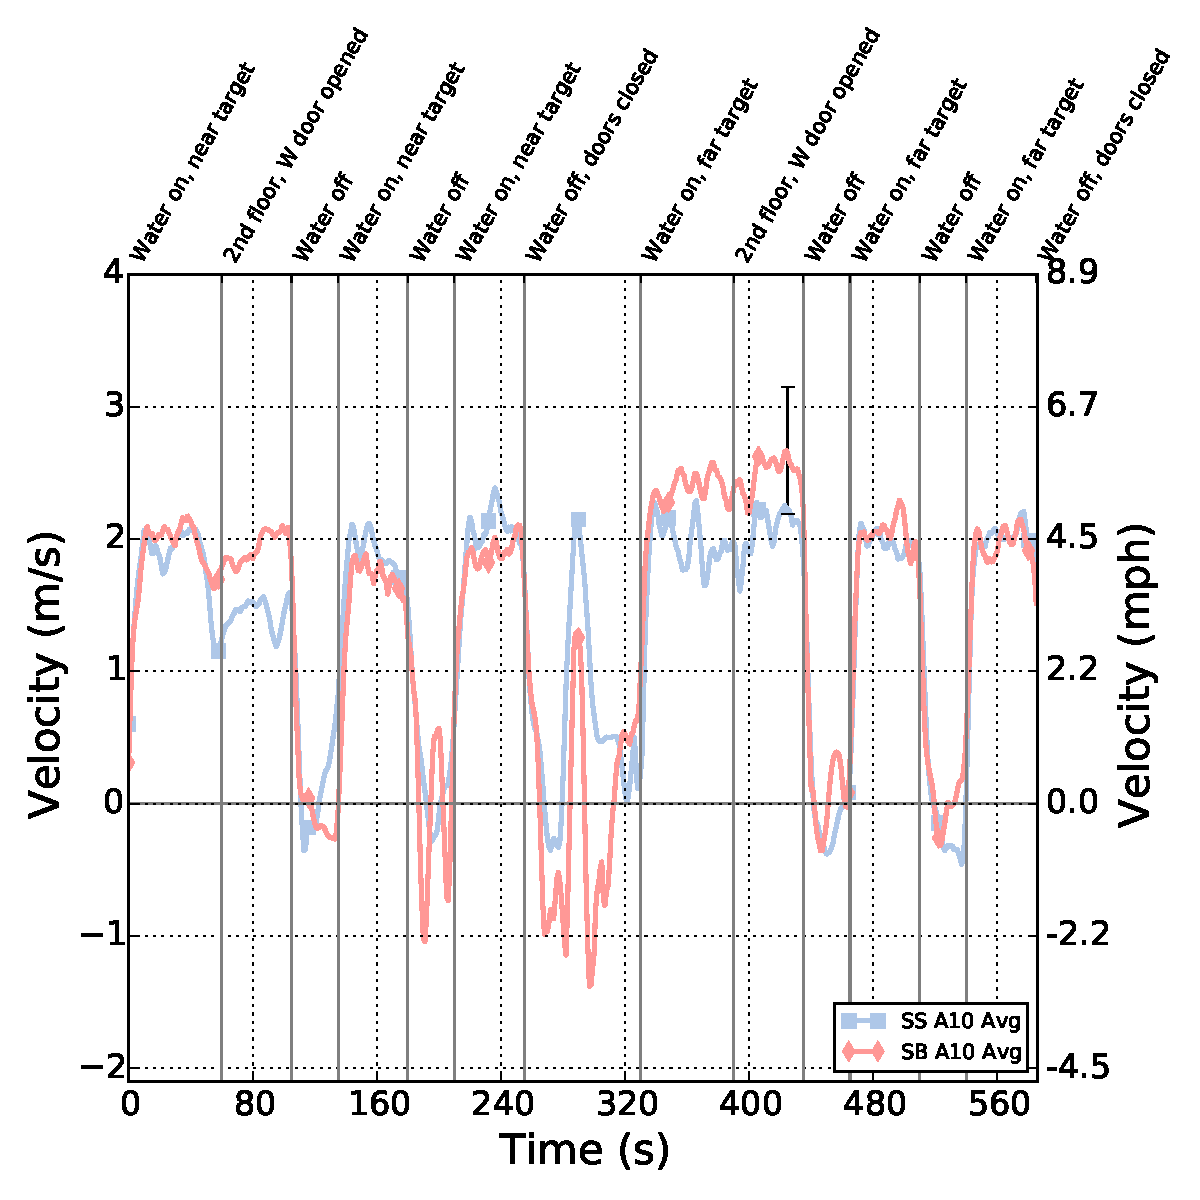
\includegraphics[width=\columnwidth]{../Figures/Plots/Test_70_West_101215_BDP_A10_stream_avgs}
	\caption[Average gas velocity through the interior stairwell door during Test~4 for the straight stream and smooth bore stream patterns.]{Average gas velocity measured by the bi-directional probes at the interior stairwell door (A10) during Test~4 for the straight stream and smooth bore stream patterns.}
	\label{fig:Test_4_BDP_A10_Avg_All}
	\end{figure}
\FloatBarrier

\chapter{Handline Test Plots}
\label{chap:handline_plots}

\begin{figure}[!ht]
	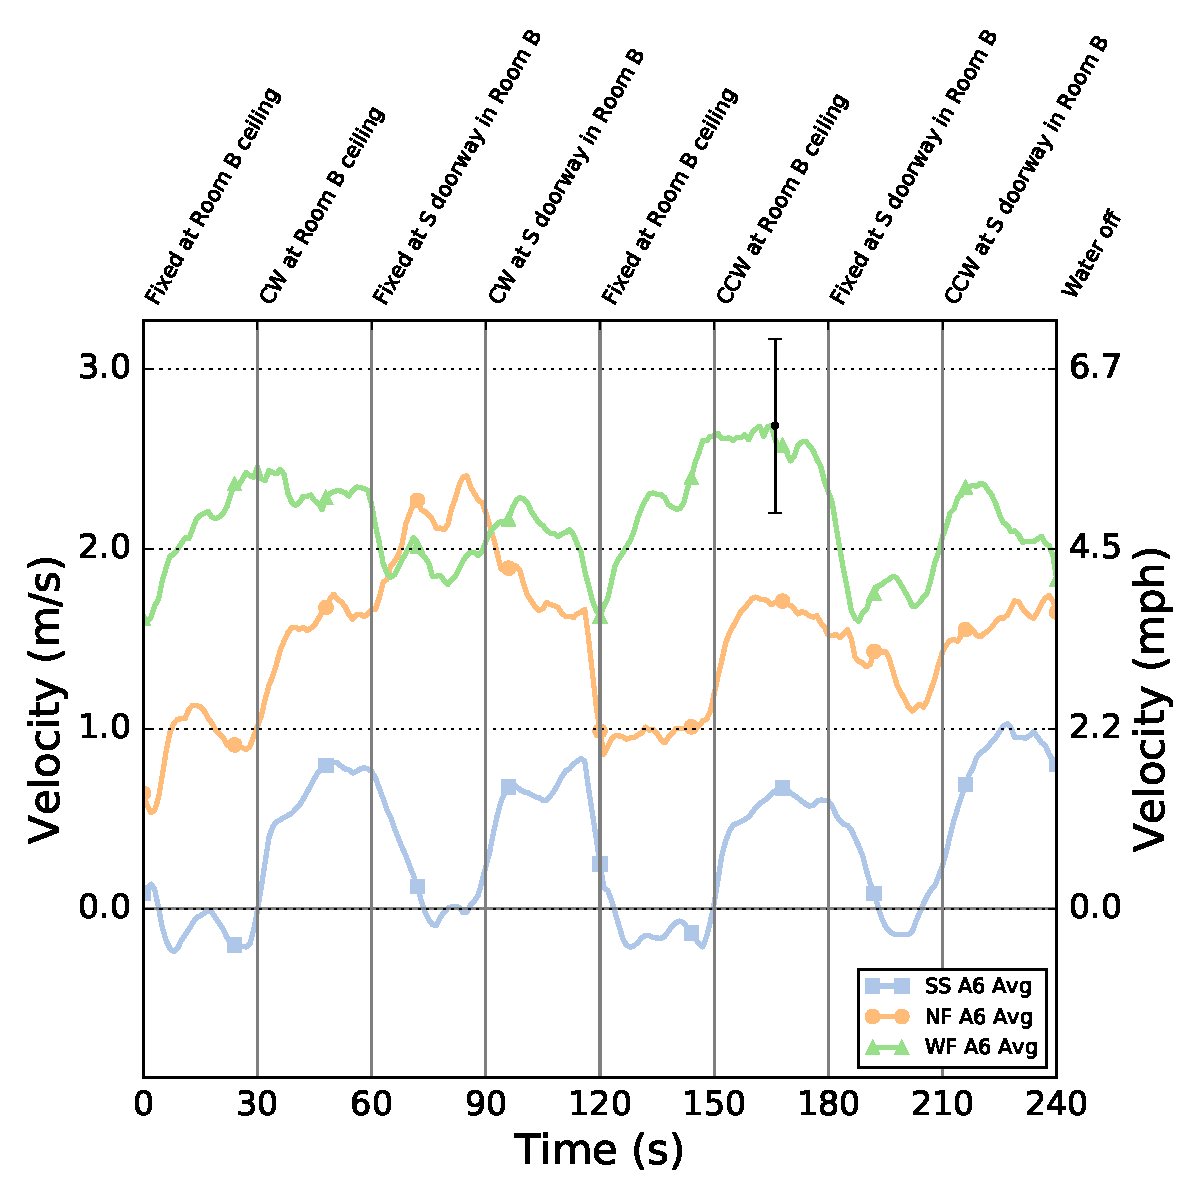
\includegraphics[width=0.86\columnwidth]{../Figures/Plots/HOSE_IXAOXX_BDP_A6_stream_avgs}
	\caption{Average velocity through stairwell door during Test~5 for three hose stream patterns.}
	\label{fig:Test_5_BDP_A6_Avg_All}
\end{figure}
\FloatBarrier

\begin{figure}[!ht]
	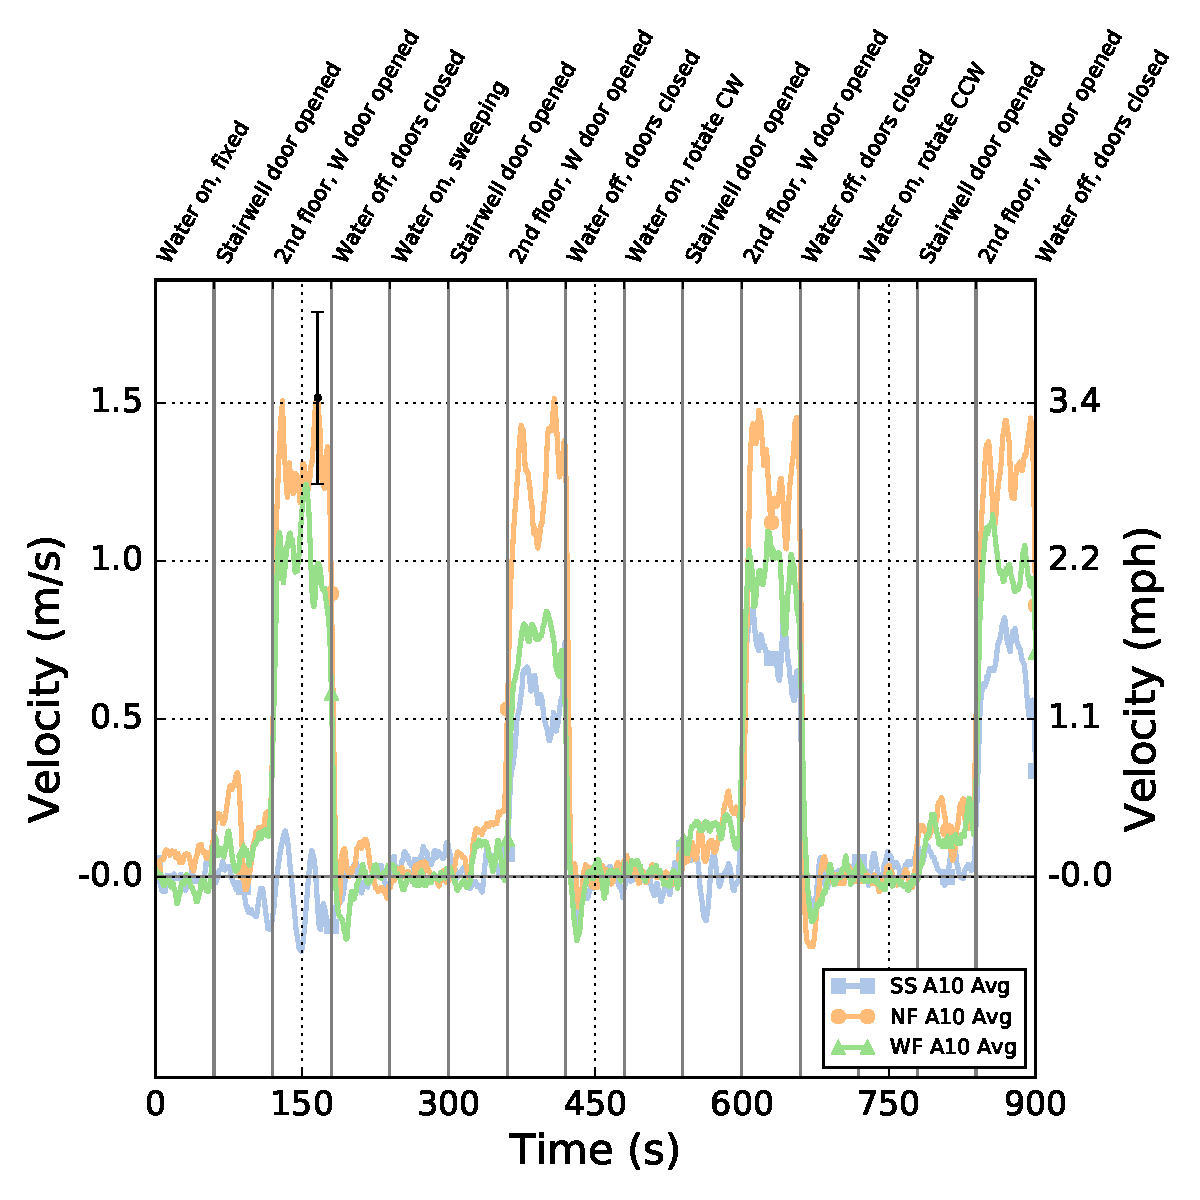
\includegraphics[width=\columnwidth]{../Figures/Plots/Test_19_West_063014_BDP_A10_stream_avgs}
	\caption{Average velocity through stairwell door during Test~7 for the three hose stream patterns.}
	\label{fig:Test_7_BDP_A10_Avg_All}
\end{figure}

\clearpage

\end{document}

